\documentclass[11pt,oneside]{book}
\usepackage{fontspec}
\usepackage{xeCJK}
\setmainfont{Latin Modern Roman}
\setCJKmainfont[ItalicFont={Noto Serif CJK SC},BoldItalicFont={Noto Serif CJK SC Bold}]{Noto Serif CJK SC}
\setCJKsansfont{Noto Sans CJK SC}
\setCJKmonofont{Noto Sans Mono CJK SC}
\newfontfamily\proseunicodefont{DejaVu Serif}
\usepackage[margin=1in]{geometry}
\usepackage{microtype}
\usepackage{amsmath,amssymb,amsthm,mathtools,bm}
\usepackage{graphicx}
\usepackage{xcolor}
\usepackage{booktabs}
\usepackage{array}
\usepackage{longtable}
\usepackage{enumitem}
\usepackage{float}
\usepackage{caption}
\usepackage{hyperref}
\usepackage{fancyhdr}
\usepackage{tikz}
\usetikzlibrary{arrows.meta,positioning,calc,decorations.pathmorphing}

\hypersetup{
  colorlinks=true,
  linkcolor=blue!50!black,
  urlcolor=blue!50!black,
  citecolor=blue!50!black
}

\setlength{\parskip}{0.5em}
\setlength{\parindent}{0pt}
\setlist[itemize]{topsep=0.25em,itemsep=0.2em}
\setlist[enumerate]{topsep=0.25em,itemsep=0.2em}
\setlength{\headheight}{40pt}
\numberwithin{equation}{chapter}

\newtheorem{theorem}{定理}[chapter]
\newtheorem{proposition}[theorem]{命题}
\newtheorem{lemma}[theorem]{引理}
\newtheorem{corollary}[theorem]{推论}
\theoremstyle{definition}
\newtheorem{definition}[theorem]{定义}
\newtheorem{example}[theorem]{例}
\theoremstyle{remark}
\newtheorem{remark}[theorem]{注}

\providecommand{\ket}[1]{\left\lvert#1\right\rangle}
\providecommand{\bra}[1]{\left\langle#1\right\rvert}
\providecommand{\braket}[2]{\left\langle#1\,\middle|\,#2\right\rangle}
\providecommand{\expect}[1]{\left\langle#1\right\rangle}
\newcommand{\lectureoverview}[1]{\paragraph{概述。} #1}
\newenvironment{classroomqa}{%
  \par\medskip
  \begin{minipage}{0.96\textwidth}
}{%
  \end{minipage}
  \par\medskip
}
\newcommand{\audiencequestion}[1]{\noindent\textbf{听众提问。} #1\par\smallskip}
\newcommand{\lecturerresponse}[1]{\noindent\textbf{回答。} #1\par}
\newcommand{\lecturetimestamp}[1]{\footnote{讲课时间： #1.}}
\newcommand{\lectureframe}[1]{\par\smallskip{\centering\footnotesize\itshape 讲课画面： #1.\par}}
\newcommand{\editorialnote}[1]{\footnote{编者说明： #1}}

\makeatletter
\newcommand{\course@headerfont}{\normalfont\small\itshape}
\newcommand{\course@pagefont}{\normalfont\small}
\newcommand{\course@headerraise}{14pt}
\newlength{\course@headerboxheight}
\setlength{\course@headerboxheight}{\dimexpr\headheight-\course@headerraise-9pt\relax}
\newcommand{\course@leftheadbox}[1]{%
  \raisebox{\course@headerraise}{%
    \parbox[t][\course@headerboxheight][t]{0.82\textwidth}{%
      \raggedright\course@headerfont\strut\MakeUppercase{#1}\strut%
    }%
  }%
}
\newcommand{\course@rightheadbox}[1]{%
  \raisebox{\course@headerraise}{%
    \parbox[t][\course@headerboxheight][t]{0.82\textwidth}{%
      \raggedleft\course@headerfont\strut\MakeUppercase{#1}\strut%
    }%
  }%
}
\renewcommand{\chaptermark}[1]{\markboth{\MakeUppercase{\chaptername\ \thechapter.\ #1}}{}}
\renewcommand{\sectionmark}[1]{\markright{\MakeUppercase{\thesection\hspace{0.4em}#1}}}
\fancyhf{}
\fancyhead[L]{\course@leftheadbox{\leftmark}}
\fancyhead[R]{\course@pagefont\thepage}
\renewcommand{\headrulewidth}{0.5pt}
\pagestyle{fancy}
\fancypagestyle{plain}{%
  \fancyhf{}
  \fancyhead[L]{\course@leftheadbox{\leftmark}}
  \fancyhead[R]{\course@pagefont\thepage}
  \renewcommand{\headrulewidth}{0.5pt}
}
\makeatother

\renewcommand{\contentsname}{目录}
\renewcommand{\chaptername}{章}
\renewcommand{\figurename}{图}
\renewcommand{\tablename}{表}
\renewcommand{\proofname}{证明}
\renewcommand{\bibname}{参考文献}
\emergencystretch=2em
\pdfstringdefDisableCommands{\def\proseunicodefont{}}

\hypersetup{
  pdftitle={Quantum Entanglement, Part 3},
  pdfauthor={Lectures by Leonard Susskind; companion edition by LazyingArt LLC},
  pdfsubject={Independently edited companion notes for the 2006 Fall lecture course},
  pdfcreator={LaTeX with hyperref}
}
\graphicspath{{../../../generated_course_notes/supplementary/quantum_entanglement/2006_fall_part_3/figures/}{../../../generated_course_notes/supplementary/quantum_entanglement/2006_fall_part_3/assets/}}
\begin{document}
\frontmatter
\hypersetup{pageanchor=false}
\begin{titlepage}
\thispagestyle{empty}
\begin{tikzpicture}[remember picture,overlay]
  \node[anchor=center,inner sep=0] at (current page.center) {%
    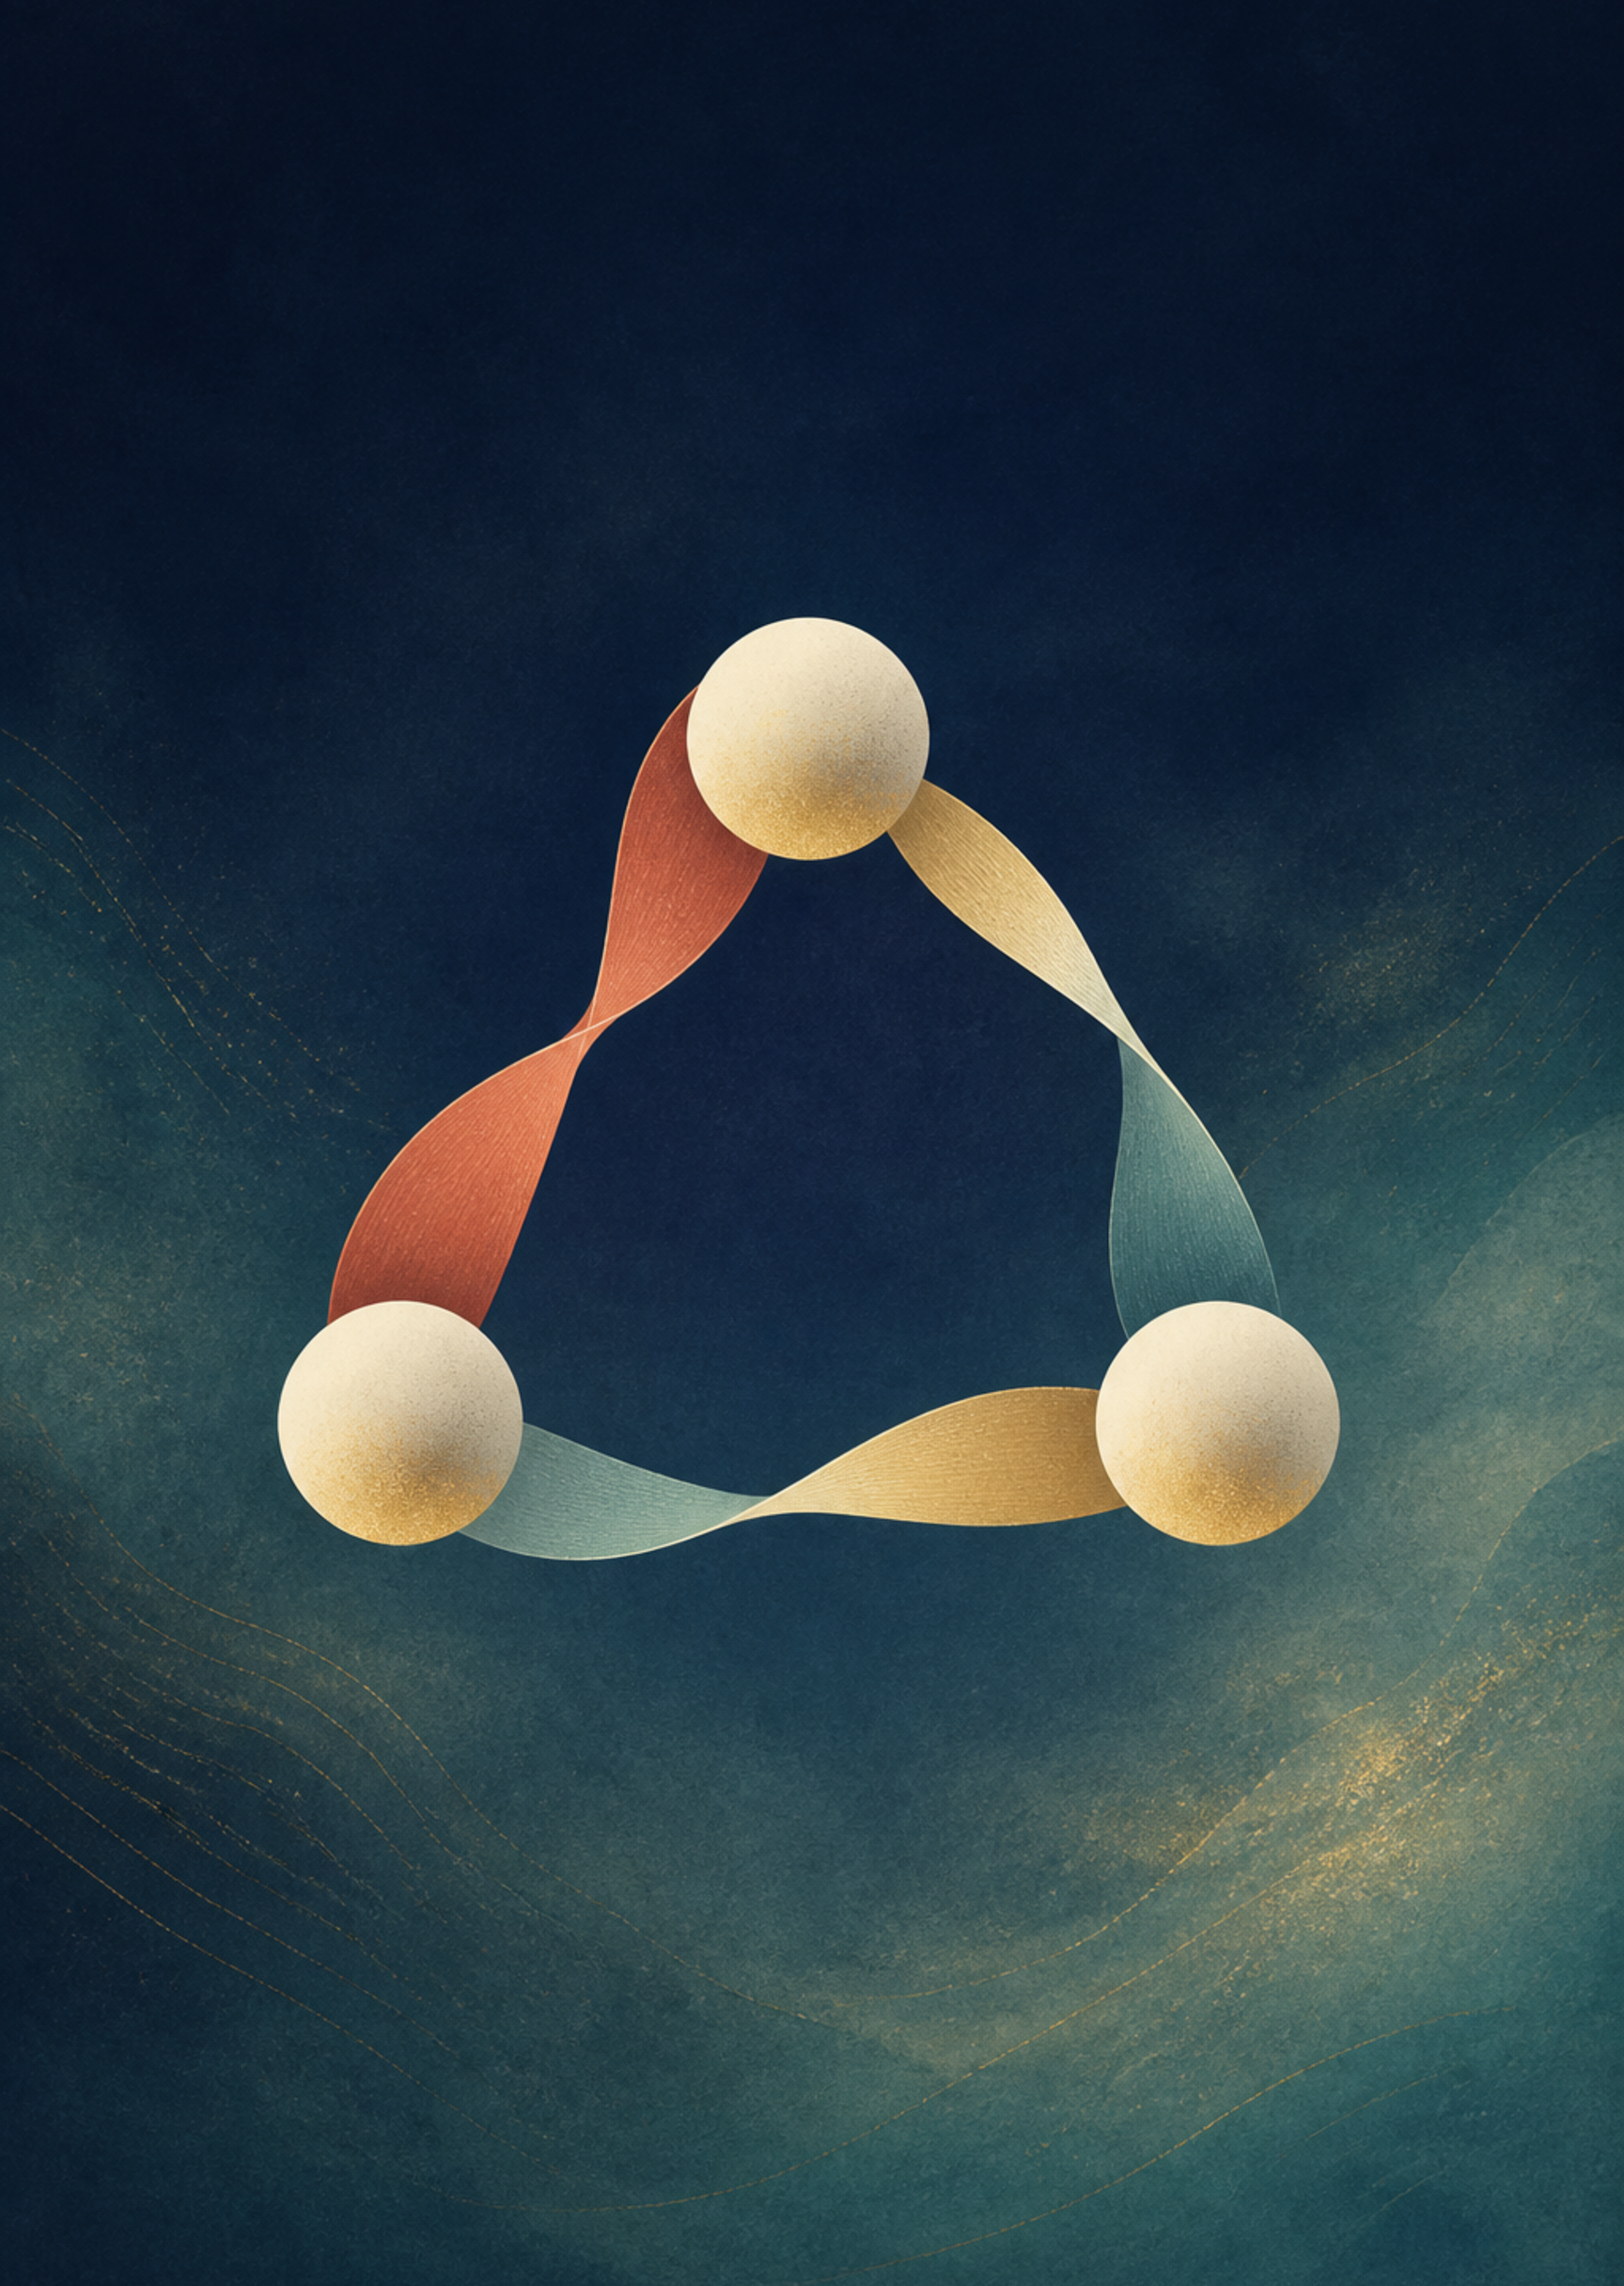
\includegraphics[height=\paperheight,keepaspectratio]{../../../generated_course_notes/supplementary/quantum_entanglement/2006_fall_part_3/assets/cover-art.png}%
  };
  \node[
    anchor=north west,
    align=left,
    text width=0.78\paperwidth,
    fill=white,
    fill opacity=0.9,
    rounded corners=8pt,
    inner xsep=10pt,
    inner ysep=8pt
  ] at ([xshift=0.08\paperwidth,yshift=-0.06\paperheight]current page.north west) {%
    {\fontsize{30}{33}\selectfont\bfseries\color{black!88} 量子纠缠 第3部\\[0.85em]}
    {\large\color{black!72} 中文版 / 2006 fall part 3}
  };
  \node[
    anchor=south west,
    align=left,
    text width=0.68\paperwidth,
    fill=white,
    fill opacity=0.82,
    text opacity=1,
    rounded corners=6pt,
    inner sep=12pt
  ] at ([xshift=0.08\paperwidth,yshift=0.08\paperheight]current page.south west) {%
    {\normalsize\color{black!78} 原讲授：Leonard Susskind\\[0.35em]}
    {\small\color{black!72} 讲义辅助版本：\href{https://lazying.art}{LazyingArt LLC} / \href{https://github.com/lachlanchen/Video2Book}{Video2Book}}
  };
\end{tikzpicture}
\mbox{}
\end{titlepage}
\hypersetup{pageanchor=true}

\clearpage
\chapter*{关于这些笔记}
这些经过独立编辑的配套笔记跟随 Leonard Susskind 的 2006 年量子纠缠讲座课程的第三部分。它们是根据机器转录、字幕和精选黑板画面重建的，然后对照可用的源材料进行了核对。它们不是 Susskind 教授的原始手稿，也未经他审阅或认可。

本版本由 \href{https://lazying.art}{LazyingArt LLC} 使用开源 \href{https://github.com/lachlanchen/Video2Book}{Video2Book} 工具包制作。机器转录仍可单独获取，可能包含识别错误。编辑性澄清和非平凡重建在脚注中标明。
\clearpage
\tableofcontents
\mainmatter
\chapter{狭义相对论：参考系、同时性与洛伦兹变换}

相对性原理是指物理定律不依赖于我们用来描述它们的惯性参考系。我们的首要任务是运动学：空间、时间、运动、同步以及从一个惯性系到另一个惯性系的变换的含义。动力学随后而来，包括相对论能量、动量、力、牛顿运动方程的类比，以及\(E=mc^2\)的含义。一旦这个结构稳固，我们就可以通过弯曲时空、粒子在给定引力场中的运动、黑洞以及宇宙膨胀，从概念上接近广义相对论，而不必从求解爱因斯坦场方程这一困难问题开始。

概念严谨性与数学严谨性之间的区别值得指出。我们不会使用明知是错误的近似。相反，我们将强调引力场对时钟、粒子和几何做了什么，同时推迟构造场方程任意解所需的工具。狭义相对论必须更明确地处理，因为所有后续推理都建立在其运动学之上。

因此，正确的起点不是某个著名的公式，而是精确说明观察者所说的位置和时间意味着什么。

\section{参考系是物理坐标系}

想象空间中充满了一个任意精细的米尺晶格。每个晶格点由三个空间坐标标记，并且在每个点都有一个时钟。这些杆和时钟共同构成了一个参考系。

\begin{definition}
一个\emph{事件}是在一个位置和一个时间发生的事情。在一维空间中，其坐标写作\((x,t)\)；在三维空间中，它们是\((x,y,z,t)\)。
\end{definition}

牛顿物理学增加了一个强有力的假设：所有理想时钟都可以一劳永逸地同步。时间是普适的。时钟可以被移动，观察者可以携带手表，但每个人都被认为在任何地方都同意同一个\(t\)。这有时被称为绝对时间；可以将其想象为上帝的时间，一个为整个世界服务的时钟。

相对性原理比爱因斯坦更古老。其自然的图景是一列在完美光滑的轨道上如此均匀地行驶的火车，以至于没有任何嘎嘎声或震动。在火车内部，我们可以像在停在车站的火车里一样抛接球。杂耍是一个令人惊讶地完整的小型力学实验：它需要计时、重力、对齐以及对轨迹的反复控制。如果火车以恒定速度行驶，这些规则都不会改变。竖直向上抛出的球会回到同一只手中；火车不会从它下面滑走。伽利略认识到了这一事实，牛顿在他的运动定律中系统地表达了它。

在伽利略之前，人们很容易推理说，移动的火车应该在球在空中时前进，迫使杂耍者向后或向前伸手去接它。错误在于忘记了球离开手时已经具有火车的水平速度。没有任何局限于平稳移动车厢内的实验能揭示绝对静止的特殊状态。只有两列火车之间的相对运动是可观察的。

因此，静止的火车和匀速运动的火车是两个惯性系。在爱因斯坦之前，它们通过伽利略变换相关联。

\section{绘制时空图}

我们暂时忽略\(y\)和\(z\)，将时间竖直绘制，位置\(x\)水平绘制。图中的每个点都是一个事件。线\(x=0\)是空间原点的历史，或\emph{世界线}。相邻的竖直线\(x=1,2,3,\ldots\)是其他晶格点的世界线。水平线是具有共同时间的事件集合。

\begin{figure}[H]
\centering
\includegraphics[width=0.62\textwidth]{lecture_01_figure_02.png}
\caption{静止参考系的时间轴和空间晶格的第一批世界线。}
\lectureframe{00:16:38}
\end{figure}

同样的构造在理想化图中更清晰：

\begin{figure}[H]
\centering
\begin{tikzpicture}[scale=0.95]
\draw[->] (-1.2,0) -- (5.2,0) node[right] {$x$};
\draw[->] (0,-0.2) -- (0,4.8) node[above] {$t$};
\foreach \x in {-1,1,2,3,4}
  \draw[gray!65] (\x,0) -- (\x,4.4);
\foreach \y in {1,2,3,4}
  \draw[gray!65] (-1.0,\y) -- (4.4,\y);
\fill (0,0) circle (1.5pt);
\node[below left] at (0,0) {$0$};
\node[left] at (0,1) {$1$};
\node[left] at (0,2) {$2$};
\node[left] at (0,3) {$3$};
\node[below] at (1,0) {$1$};
\node[below] at (2,0) {$2$};
\node[below] at (3,0) {$3$};
\end{tikzpicture}
\caption{一个静止的时空晶格。竖直线具有恒定位置；水平线具有恒定时间。}
\end{figure}

网格是想象的，其间距是任意的。我们可以使用米、厘米、微米或任何更小且具有物理意义的间隔。其目的是为每个事件分配精确的坐标。

“参考系”这个说法现在有了可操作的内容。它不仅仅是一个视角，或某个朝某个方向看的人。它是一个延展的坐标装置。给定一个事件，当地的尺子指明它发生在哪里，当地的钟指明它发生在何时。于是其他物理量就可以在不同参考系之间进行比较：一个粒子的位置和速度、它的能量、也许还有一个物体的温度，最终还有它的动量和力。最简单的比较是涉及\(x\)和\(t\)的那一种，所以我们就从那里开始。

现在，在一列沿\(x\)正方向以恒定速度\(v\)行驶的火车上放置第二套格点。选择两原点在\(t=0\)时重合。于是运动的原点遵循
\begin{equation}
x=vt.
\end{equation}
固定在火车上的其他每一个点都遵循一条平行的倾斜世界线。这种倾斜不过是如下几何陈述：火车随时间推移而改变位置。

假设火车尾部的点是带撇原点。在\(t=0\)时，它与车站原点重合。在较晚的时刻\(t\)，它的静止坐标为\(vt\)。因此，一个位于坐标\(x\)附近的事件距离火车原点只有\(x-vt\)。这就是为什么该变换是一次减法，而不是一条任意的代数规则。

设\((x,t)\)为一个事件在车站系中的坐标，\((x',t')\)为它在火车系中的坐标。伽利略和牛顿保留普适时间，
\begin{equation}
t'=t.
\end{equation}
在时间\(t\)内，运动的原点前进\(vt\)，所以从该原点到该事件的距离为
\begin{equation}
x'=x-vt.
\end{equation}
合起来，
\begin{align}
t'&=t, & x'&=x-vt.
\label{eq:galilean-forward}
\end{align}
解出不带撇的坐标，就得到逆变换，
\begin{align}
t&=t', & x&=x'+vt'.
\label{eq:galilean-inverse}
\end{align}

\begin{figure}[H]
\centering
\includegraphics[width=0.72\textwidth]{lecture_01_figure_03.png}
\caption{与两个时空格点并列写出的伽利略变换。}
\lectureframe{00:21:57}
\end{figure}

第一对公式告诉运动的观察者如何转换静止观察者提供的坐标。逆变换那一对则转换回去。这种在两种描述之间的相互转换，就是伽利略相对论的数学内容。

在逆空间公式中作替换\(t\to t'\)之所以无害，只是因为伽利略理论已经宣告了\(t=t'\)。现在注意到这个假设是有益的。在爱因斯坦的理论中，两个时间坐标将不同，而这样的替换将不再是自动成立的。

\begin{classroomqa}
\audiencequestion{如果一只钟被带走，然后又被带回来，我们怎么能知道它的运动没有先使它变快、然后又使它变慢，从而在比较这些钟时把效应掩盖起来呢？
\lecturetimestamp{00:23:09}}
\lecturerresponse{伽利略不可能以现代精度确立普适时间；那是一个物理猜测。我们可以用许多方式检验这个猜测：把好钟沿相反方向携带，把北--南之行以及东--西之行都重复，让一只钟绕另一只钟运动，或者在不把钟放在一起的情况下交换授时信号。在普通速度下，所有这类检验都以极高精度一致。有了足够精确的钟，或者足够大的速度，就会出现一个微小的偏差。普适时间的这种失效并不是实验的缺陷；它是狭义相对论必须解释的现象之一。}
\end{classroomqa}

\section{伽利略不变量与牛顿定律}

不变量是所讨论的所有惯性观察者都同意的一个量。坐标本身不必是不变量。要紧的是，由它们组装出来的定律是否保持相同的形式。

这个词既用作名词，也用作形容词。一个数可以是不变量，而一个方程可以在某个变换下是不变的。不变量与不变定律之间的区分防止了一种常见的混淆：相对论并不主张每个观察者对一切事物都得到相同的坐标。它主张的是，联系他们测量结果的物理定律具有相同的形式。

取两个同时发生的事件，位置分别为\(x_1\)和\(x_2\)。方程~\eqref{eq:galilean-forward}给出
\begin{align}
x_1'&=x_1-vt,\\
x_2'&=x_2-vt.
\end{align}
因此它们的间隔为
\begin{equation}
x_2'-x_1'=(x_2-vt)-(x_1-vt)=x_2-x_1.
\end{equation}
在伽利略物理学中，同时发生的事件之间的距离是不变量，尽管各个位置本身不是。

\begin{classroomqa}
\audiencequestion{那个减法中出现的两个\(t\)真的是同一个时间吗？
\lecturetimestamp{00:28:16}}
\lecturerresponse{是的。我们特意选择这两个事件为\((x_1,t)\)和\((x_2,t)\)。它们位于同一条水平的等时线上。因此公共项\(vt\)相消。如果这些事件发生在不同时间，这个论证就不会确立一个不变的空间间隔。}
\end{classroomqa}

现在用轨迹\(x(t)\)描述一个粒子。列车观察者给出
\begin{equation}
x'(t)=x(t)-vt.
\end{equation}
求一次导数便得到熟悉的速率相加法则，
\begin{equation}
\frac{dx'}{dt}=\frac{dx}{dt}-v.
\end{equation}
位置和速率依赖于参考系。与一支箭并排运动的观察者看到它行进得比站在轨道旁的观察者更慢。

再求一次导数。由于相对速率\(v\)是常量，
\begin{equation}
\frac{d^2x'}{dt^2}=\frac{d^2x}{dt^2}.
\end{equation}
加速度在伽利略变换下不变。这有力地提示了为什么牛顿定律用加速度而不是位置或速率来书写。

这是被观测物体的加速度，而不是列车观察者的加速度。两个参考系都是惯性的，因此两个参考系彼此之间都不加速。物体在任一种描述中都可能向左或向右加速，而两个观察者对该加速度的数值一致，尽管他们对物体的位置和速率并不一致。

假设两个粒子彼此施加一个力，且该力只依赖于它们在同一时刻的间距。该间距是不变量，因此该力也是不变量。如果质量同样是一种内禀的、与参考系无关的性质，那么每个惯性观察者都能以完全相同的形式写出
\begin{equation}
F=ma
\end{equation}
牛顿力学在伽利略变换下不变。这不仅仅看似合理；在通常速率的整个范围内，它都极其精确。

该论证适用于熟悉的有心力，例如牛顿引力或静电作用，其中大小是距离的函数。由于所有伽利略观察者在同一时刻对该距离一致，他们对该力也一致。在力和加速度都确定的情况下，一致性进而要求他们对质量也一致：一个1千克的物体被列车带过时仍然是一个1千克的物体。\(F=ma\)中的每个符号都符合同样的不变结构。

\section{光不符合伽利略法则}

电磁学造成了困难。麦克斯韦方程组预言波以确定速率\(c\)穿过真空传播。如果麦克斯韦方程组是自然定律，而自然定律在每个惯性参考系中都相同，那么所有惯性观察者都必须得到相同的\(c\)。

伽利略运动学预言了别的东西。在静止参考系中向右运动的光脉冲满足
\begin{equation}
x=ct.
\end{equation}
施加空间变换得到
\begin{equation}
x'=x-vt=(c-v)t.
\end{equation}
由于\(t'=t\)，列车观察者将测得速率\(c-v\)。

这一矛盾可以尖锐地陈述出来。如果麦克斯韦方程组保持其形式，它们就在带撇参考系中预言\(c\)。如果保留伽利略变换，它就预言\(c-v\)。当\(v\ne0\)时，两者不可能都精确成立。

如果光在介质中的行为像普通波，这个结果看起来就完全自然。随水波运动的船测得较低的相对波速。在静止空气中运动的听者测得的声速会因听者相对于空气的运动而发生偏移。因此，19世纪的物理学家被引向一个优先的静止状态，即一个以太参考系，在其中麦克斯韦方程组具有其最简单形式，而光以\(c\)运动。旨在探测相对于这样一个优先参考系的运动的实验没有发现相应的效应。

有若干种可能的实验安排，但它们的共同目标是比较处于不同运动状态或方向的观察者所看到的光传播。没有一个实验揭示出预期的伽利略偏移。这一失败并不是小小的技术麻烦。它迫使人们在相对性原理、麦克斯韦方程组以及继承下来的空间和时间观念之间做出选择。

爱因斯坦更直接地处理这一冲突。年轻时，他想象追逐一列光波。如果他能追上它，它振荡的电磁图样就会冻结在空间中，然而麦克斯韦方程组不允许这样的静止光波。他选择把麦克斯韦理论和相对性原理视为基本的，然后重新审视隐藏在我们的坐标中的假设。

这一重建基于两条公设：
\begin{enumerate}
\item 物理定律在每个惯性参考系中都具有相同的形式。
\item 真空中的光在每个惯性参考系中都具有相同的速率\(c\)。
\end{enumerate}

第二条公设不能与伽利略变换共存。某种比速度相加法则更深层的东西必须改变。爱因斯坦的简洁选择是保留这两条公设，并重新审视那个看似无害的伽利略方程\(t'=t\)。

\section{同步远处的钟}

空间距离可以用杆来铺设，但远处的钟需要一种同步约定。把两个钟放在与中点观察者等距的位置。当每个端点处的钟读到约定时刻时，让它发出一次闪光。如果两次闪光同时到达中点，就称端点处的钟已同步。如果一次闪光先到达，就调整相应的钟并重复该程序。

“\emph{中点}”一词是用该参考系中已经铺设好的杆来定义的。因此这个检验包含两个彼此独立的要素：到两端点的空间距离相等，以及信号到达时间相等。两个要素都不能省略。在整个格点上重复该程序，就提供了牛顿曾直接假定的水平等时线。

这个定义使用光，是因为该公设赋予光在每个惯性系中相同的速度。一旦所有相邻的钟对都按这种方式处理完毕，整个格点就带有一族同步的钟。

现在让第二个格点穿过第一个格点运动。运动装置的中点在它自己的参考系中仍位于两个运动端点之间的中点。然而，相对于静止装置，它朝着一束迎面而来的闪光运动，并远离另一束闪光。按照静止钟同时发出的闪光，并不会同时到达运动的中点。由于运动的观察者应用同样的中点与光规则，该观察者不能称那些发射是同时的。每个参考系都一致地同步自己的钟，但这两个同步方案并不一致。

这并不是由光的有限传播时间造成的光学错觉。每个观察者都知道光需要时间才能到达，并用相同的速度\(c\)对此进行修正。修正之后分歧仍然存在，因为观察者并不会把同样的远处事件选为一对同时事件。相对的正是同时性本身，而不只是同时性的表象。

\begin{classroomqa}
\audiencequestion{我们能否改用声音而不是光来同步钟，从而避免这个结论？
\lecturetimestamp{00:49:03}}
\lecturerresponse{在空气静止的参考系中，声音可以作为同步信号，但在每个惯性系中测得的声音速度并不相同。一列穿过静止空气的敞篷列车相对于传声介质在运动，因此向前和向后的声音信号在那里并不对称。光按公设则不同：不存在可探测的光学介质，其静止参考系会选出一个观察者。因此我们使用光，并遵循其后果。}
\end{classroomqa}

定性上的分歧已经清楚。现在我们来精确计算运动观察者称哪些事件为同时事件。

\section{光线的构造}

为了进行构造，方便的做法是选择如下单位：
\begin{equation}
c=1.
\end{equation}
于是，一个距离单位就是光在一个时间单位内走过的距离：光秒与秒配对，或光年与年配对。空间和时间带有相同的单位，速度是无量纲的，光线出现在\(45^\circ\)处。向右运动的光线有
\begin{equation}
x=t+d,
\end{equation}
而向左运动的光线有
\begin{equation}
x=-t+d'.
\end{equation}
过原点的两条光线就分别是\(x=t\)和\(x=-t\)。属于比光慢的物体的类时轨迹，更靠近竖直轴。假设的超光速轨迹则会更靠近水平轴。

图中的角度只有在这种单位选择之后才有意义。若用米和秒，光线看起来几乎水平，因为它在1秒内大约走过\(3\times10^8\)米。选择光秒作为距离会重新标定水平轴，并使因果几何变得可见。

考虑运动格点中的三条平行世界线，
\begin{equation}
x=vt,\qquad x=vt+L,\qquad x=vt+2L.
\label{eq:moving-worldlines}
\end{equation}
中间的世界线属于那个检验两个外侧点之间同时性的观察者。这三个点都匀速运动，并在带撇参考系中保持它们的相对排列。

\begin{figure}[H]
\centering
\includegraphics[width=0.72\textwidth]{lecture_01_figure_04.png}
\caption{向右的光线\(x=t\)与中间运动世界线相交。}
\lectureframe{01:02:33}
\end{figure}

完整的几何可以画出来，而不必受站在黑板前的人的妨碍：

\begin{figure}[H]
\centering
\begin{tikzpicture}[scale=0.95]
\draw[->] (-0.5,0) -- (6.5,0) node[right] {$x$};
\draw[->] (0,-0.2) -- (0,4.3) node[above] {$t$};
\draw[blue] (0,0) -- (1.4,4.0);
\draw[blue] (2.0,0) -- (3.4,4.0);
\draw[blue] (4.0,0) -- (5.4,4.0);
\draw[red] (0,0) -- (3.08,3.08);
\draw[red] (3.08,3.08) -- (4.56,1.60);
\draw[red,dashed] (2.0,0) -- (4.56,1.60);
\fill (0,0) circle (1.5pt);
\fill (2.0,0) circle (1.5pt);
\fill (4.0,0) circle (1.5pt);
\fill (3.08,3.08) circle (1.5pt);
\fill (4.56,1.60) circle (1.5pt);
\node[left] at (0.55,1.55) {$x=vt$};
\node[left] at (2.45,1.9) {$x=vt+L$};
\node[right] at (4.72,1.9) {$x=vt+2L$};
\node[left] at (1.88,2.28) {$x=t$};
\node[above right] at (3.08,3.08) {$A$};
\end{tikzpicture}
\caption{光信号决定运动参考系的等时线。}
\end{figure}

从原点发出一束向右运动的光线。设\(A\)为它与中间世界线的交点。\(A\)处的两个方程是
\begin{align}
x&=t,\\
x&=vt+L.
\end{align}
代入得到
\begin{equation}
t=vt+L,
\end{equation}
因此
\begin{equation}
t_A=x_A=\frac{L}{1-v}.
\label{eq:point-a}
\end{equation}

从\(A\)出发，沿一条向左运动的光线反向追溯到最右侧的运动世界线。其方程具有如下形式
\begin{equation}
x+t=b.
\end{equation}
由于它经过\(A\)，方程~\eqref{eq:point-a}确定了常数：
\begin{equation}
b=x_A+t_A=\frac{2L}{1-v}.
\end{equation}
因此这条反向光线满足
\begin{equation}
x+t=\frac{2L}{1-v}.
\label{eq:backward-ray}
\end{equation}

它与最右侧世界线的交点可由下式得到
\begin{align}
x+t&=\frac{2L}{1-v},\\
x&=vt+2L.
\end{align}
消去\(x\)，
\begin{align}
(1+v)t
  &=2L\left(\frac{1}{1-v}-1\right)\\
  &=\frac{2Lv}{1-v},
\end{align}
所以
\begin{equation}
t=\frac{2Lv}{1-v^2}.
\end{equation}
代入\(x=vt+2L\)得到
\begin{equation}
x=\frac{2L}{1-v^2}.
\end{equation}
坐标本身不如它们的比值重要：
\begin{equation}
\frac{t}{x}=v.
\end{equation}
因此，按照运动时钟与原点同时的每一个事件都位于
\begin{equation}
t=vx,
\label{eq:simultaneity-c-one}
\end{equation}
而运动的原点则沿
\begin{equation}
x=vt.
\label{eq:moving-time-axis}
\end{equation}
这两条轴关于\(45^\circ\)光线对称地倾斜。

\(x=vt\)上的所有点都具有相同的带撇位置，\(x'=0\)，而它们的带撇时间各不相同。\(t=vx\)上的所有点都具有相同的带撇时间，\(t'=0\)，而它们的带撇位置各不相同。因此，其中一条线是带撇时间轴，另一条是带撇空间轴。需要借助长信号构造来确定第二条线；仅凭运动世界线无法推断出它。

在方程~\eqref{eq:simultaneity-c-one}中恢复普通单位需要
\begin{equation}
t=\frac{v}{c^2}x.
\label{eq:simultaneity-dimensional}
\end{equation}
因子\(c^2\)解释了为什么牛顿图像在日常生活中如此有效。对于远小于\(c\)的速度，运动同时线的斜率极小。

\begin{figure}[H]
\centering
\includegraphics[width=0.72\textwidth]{lecture_01_figure_05.png}
\caption{当\(c=1\)时，带撇时间轴与同时轴关于光线对称。}
\lectureframe{01:15:40}
\end{figure}

\begin{figure}[H]
\centering
\begin{tikzpicture}[scale=1.0]
\draw[->] (-2.2,0) -- (5.2,0) node[right] {$x$};
\draw[->] (0,-0.2) -- (0,4.9) node[above] {$t$};
\draw[red] (0,0) -- (3.9,3.9);
\draw[red] (0,0) -- (-1.8,1.8);
\draw[blue] (0,0) -- (1.8,4.5);
\draw[blue,dashed] (0,0) -- (4.5,1.8);
\node[right] at (3.9,3.9) {$x=t$};
\node[left] at (-1.8,1.8) {$x=-t$};
\node[above] at (1.8,4.5) {$x'=0$};
\node[right] at (4.5,1.8) {$t'=0$};
\end{tikzpicture}
\caption{以\(c=1\)为单位的带撇轴与不变光线。}
\end{figure}

\section{推导洛伦兹变换}

几何结构确定了每个带撇坐标在何处为零。沿运动时间轴\(x=vt\)，必须有\(x'=0\)。沿运动同时轴\(t=vx\)，必须有\(t'=0\)。具有这些零集的最一般线性关系可以写成
\begin{align}
x'&=\frac{x-vt}{F(v)},\\
t'&=\frac{t-vx}{G(v)}.
\label{eq:fg-ansatz}
\end{align}
因子\(F\)和\(G\)允许带撇坐标的标度不同于伽利略标度，即使两条轴的位置已经确定。线性来自空间和时间的均匀性：平移一个实验不可能改变变换律。\editorialnote{这个简短的线性论证明确指出了黑板推导中隐含使用的一个假设。}

在这个阶段，几何已经告诉了我们很多，但并非全部。分子确定了轴的倾斜。它们并未确定沿这些轴的单位间距。那部分剩余的标度信息正是\(F(v)\)和\(G(v)\)所表示的。

现在施加光速不变性。一条满足\(x=t\)的向右运动光线也必须满足\(x'=t'\)。沿这条光线，
\begin{align}
x'&=\frac{(1-v)t}{F(v)},\\
t'&=\frac{(1-v)t}{G(v)}.
\end{align}
对光线上每一点都相等要求
\begin{equation}
F(v)=G(v).
\end{equation}
因此我们可以写出
\begin{align}
x'&=\frac{x-vt}{F(v)},\\
t'&=\frac{t-vx}{F(v)}.
\label{eq:common-f}
\end{align}

这一步在代数中使用了第一个真正属于爱因斯坦的要求。同一条几何直线对两个观察者都是光线，因此当\(c=1\)时，沿它两个带撇坐标必须等量增加。若两个方程中的因子不同，带撇速度就会不等于1。

还剩一个未知函数。将方程~\eqref{eq:common-f}乘以\(F(v)\)：
\begin{align}
F(v)x'&=x-vt,\\
F(v)t'&=t-vx.
\end{align}
将第二个方程乘以\(v\)并与第一个相加，消去\(t\)，得到
\begin{equation}
(1-v^2)x=F(v)(x'+vt').
\end{equation}
类似地，
\begin{equation}
(1-v^2)t=F(v)(t'+vx').
\end{equation}
因此逆变换为
\begin{align}
x&=\frac{F(v)}{1-v^2}(x'+vt'),\\
t&=\frac{F(v)}{1-v^2}(t'+vx').
\end{align}

相对性原理使两个参考系互为对等。如果车站看到列车以\(+v\)运动，那么列车看到车站以\(-v\)运动。因此，逆方程必须与正方程具有相同形式，只是\(v\)的符号相反。它们的前置因子必须满足
\begin{equation}
\frac{F(v)}{1-v^2}=\frac{1}{F(v)}.
\end{equation}
因此
\begin{equation}
F(v)^2=1-v^2,
\end{equation}
而在\(v=0\)处与恒等变换的连续性选出正根，
\begin{equation}
F(v)=\sqrt{1-v^2}.
\end{equation}

没有任何东西是针对某个特定光脉冲拟合出来的。这个结果来自由同步确定的两条轴、共同的光速，以及要求两个惯性系都不比另一个更特殊。

在\(c=1\)的单位制下，洛伦兹变换为
\begin{align}
x'&=\frac{x-vt}{\sqrt{1-v^2}},\\
t'&=\frac{t-vx}{\sqrt{1-v^2}}.
\label{eq:lorentz-c-one}
\end{align}
其逆变换为
\begin{align}
x&=\frac{x'+vt'}{\sqrt{1-v^2}},\\
t&=\frac{t'+vx'}{\sqrt{1-v^2}}.
\end{align}

\begin{figure}[H]
\centering
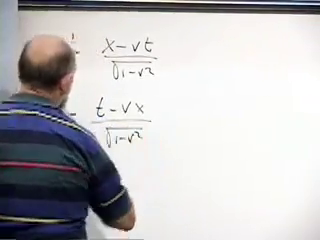
\includegraphics[width=0.76\textwidth]{lecture_01_figure_06.png}
\caption{黑板上完成的\(c=1\)洛伦兹变换。}
\lectureframe{01:32:38}
\end{figure}

本质上的新意已经在时间方程中显现出来。时间并不是简单地从一个参考系原样带到另一个参考系。带撇时间坐标混合了不带撇时间和位置。因此，\(t=\text{constant}\)和\(t'=\text{constant}\)描述的是不同的若干事件集合。

混合项并不是事后附加的可选修正。没有它，\(t'=0\) 这条线就会保持水平，异地同时性就会保持普适，而该变换也无法保持光速。

\section{恢复光速并检验结果}

当 \(c\ne1\) 时，量纲一致性会补回缺失的因子。比值 \(v^2/c^2\) 是无量纲的，而 \((v/c^2)x\) 具有时间的量纲。因此
\begin{align}
x'&=\frac{x-vt}{\sqrt{1-v^2/c^2}},\\
t'&=\frac{t-(v/c^2)x}{\sqrt{1-v^2/c^2}}.
\label{eq:lorentz-dimensional}
\end{align}
将 \(v\) 的符号反转，就得到逆变换：
\begin{align}
x&=\frac{x'+vt'}{\sqrt{1-v^2/c^2}},\\
t&=\frac{t'+(v/c^2)x'}{\sqrt{1-v^2/c^2}}.
\end{align}
引入
\begin{equation}
\gamma=\frac{1}{\sqrt{1-v^2/c^2}}
\end{equation}
会把这些式子写成熟悉的紧凑形式，但分母形式使推导过程保持可见。

数值上，\(c\simeq3\times10^8\,\mathrm{m/s}\)，所以 \(c^2\simeq9\times10^{16}\,\mathrm{m^2/s^2}\)。巨大的分母使得同时性倾斜和因子 \(v^2/c^2\) 在大多数力学实验中都难以察觉。它们的微小性解释了伽利略的成功；但这并不能恢复绝对时间。

\begin{figure}[H]
\centering
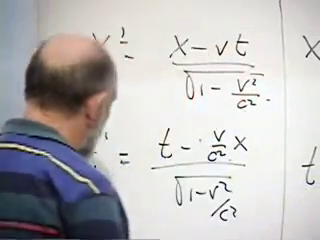
\includegraphics[width=0.76\textwidth]{lecture_01_figure_07.png}
\caption{恢复 \(c\) 的因子之后的洛伦兹变换。}
\lectureframe{01:35:58}
\end{figure}

两项检验立即可得。首先取 \(v\ll c\)。于是 \(v^2/c^2\) 可以忽略，而对于通常的距离，同时性相对性项 \(vx/c^2\) 也可以忽略。式~\eqref{eq:lorentz-dimensional} 化为
\begin{equation}
t'\approx t,\qquad x'\approx x-vt.
\end{equation}
伽利略相对性作为低速近似被重新得到。

其次，检验一条光线。一旦 \(c\) 被恢复，向右运动的光线满足 \(x=ct\)，而不是 \(x=t\)。代入给出
\begin{align}
x'&=\frac{(c-v)t}{\sqrt{1-v^2/c^2}},\\
t'&=\frac{(1-v/c)t}{\sqrt{1-v^2/c^2}}.
\end{align}
由于 \(c-v=c(1-v/c)\)，
\begin{equation}
x'=ct'.
\end{equation}
带撇的观察者测得相同的速率 \(c\)。对于向左运动的光线，代入 \(x=-ct\) 同样给出
\begin{equation}
x'=-ct'.
\end{equation}
该变换正确地处理了沿任一方向运动的光。

\(x=t\) 与 \(x=ct\) 之间的区别是一个有启发性的量纲检验。前者仅在 \(c=1\) 的单位制下才是正确的。如果在变换中恢复通常单位，却把光线方程留在自然单位中，就会混合两种约定并产生错误结果。量纲一致性会立刻抓住这个错误。

\section{中点判据}

\begin{classroomqa}
\audiencequestion{假设一个观察者在同一瞬间接收到两次闪光，但他并不位于两个光源之间的中点。这个观察者可以断定两次闪光是同时发出的吗？
\lecturetimestamp{01:42:55}}
\lecturerresponse{不可以。只有当观察者在相关参考系中空间上位于两个光源的正中间时，相同的到达时间才意味着相同的发射时间。一个更靠近某个光源的接收者可以同时接收到两次闪光，即使较远的那次闪光发射得更早。因此在运动构造中，中点世界线 \(x=vt+L\) 是必不可少的。向前光线 \(x=t\) 被追踪到它与该中点相遇，然后一条向后光线被追溯到 \(x=vt+2L\)。按照运动参考系，与原点同时的是第二个端点事件，而不是别处任意一个到达时间相同的事件。}
\end{classroomqa}

我们已经得到了完整的坐标变换，但还没有得到它最熟悉的推论。接下来是长度收缩、时间膨胀和固有时，然后是相对论动量和能量。基础已经就位：每个惯性系之所以可以使用相同的定律并测得相同的光速，只是因为空间和时间会混合，而且异地同时性属于某个参考系，而不是绝对地属于世界。
\chapter{麦克斯韦方程组、协变性与电磁波}

\lectureoverview{电场和磁场通过洛伦兹力作用于带电物质，但物质也必须产生并重新排布场。我们将表述电磁学的这另一半互易关系，证明麦克斯韦方程组是洛伦兹协变的，导出其波动解，然后以使局域守恒显而易见的形式重新引入电荷和电流。在整个讲座中，我们使用\(c=1\)的单位制。}

\section{电磁学的另一半}

从已经掌握的那部分内容开始。若一个电荷为\(q\)的粒子以速度\(\mathbf v\)穿过电场和磁场，则力为
\begin{equation}
\mathbf F=q\bigl(\mathbf E+\mathbf v\times\mathbf B\bigr).
\label{eq:lorentz-force-three}
\end{equation}
因子\(q\)不可或缺。不带电的粒子感受不到电磁力。即使粒子瞬时静止，电场也有贡献，而磁场的贡献则取决于其运动。

方程~\eqref{eq:lorentz-force-three}告诉我们给定的场对物质做了什么。它并未告诉我们是什么决定了场。是什么在一个物体周围产生电场、在另一个物体周围产生磁场，或产生一个在真空中传播的波？回答这些问题的方程就是麦克斯韦方程组。

\begin{figure}[H]
\centering
\includegraphics[width=0.62\textwidth]{lecture_58_figure_02.png}
\caption{三矢量洛伦兹力及其张量重述的开端。}
\lectureframe{00:05:49}
\end{figure}

力定律的相对论形式预示了我们所需的记号：
\begin{equation}
f^\mu=qF^\mu{}_{\nu}u^\nu.
\label{eq:lorentz-force-four}
\end{equation}
这里\(u^\nu\)是四维速度，\(f^\mu\)是四维力，而\(F^{\mu\nu}\)是由\(\mathbf E\)和\(\mathbf B\)组装成的反对称张量。黑板上首先只显示了这个表达式的示意性开端；与\(u^\nu\)的缩并提供了留下一个自由力指标所需的缺失矢量。

物质必须反作用于场，这有一个物理上的理由。电磁波可以击中一个电荷，使其加速，并把能量传递给它。如果场能影响电荷，而电荷却永远不能影响场，那么这份能量就没有来源可供抽取。作用与反作用并不完全是全部论证，但能量守恒使这种互易耦合不可避免。

\section{变化的源发出扰动}

一个点电荷产生一个从其位置向外或向内指向的电场。导线中的电流--带电粒子的流动--产生一个环绕导线环流的磁场。这些熟悉的静态图像已经显示出两种不同的几何模式：电通量从电荷发出，而磁感线则绕电流缠绕。

现在突然移动这个点电荷。在其新位置附近，电场必须开始重新排布，但远处的观察者无法立即得知这一运动。在信号有时间到达之前，旧的场仍留在远处。在近区和远区之间，存在一个场正在变化的移动前沿。这种移动的重新排布就是一种电磁扰动。

如果电荷被来回驱动，相继的重新排布便一个接一个地发生，形成电磁波。这就是天线的基本功能：振荡的电流向外发出场的扰动。使导线中的电流反向，就给出同一论证的磁版本。\(\mathbf B\)的环流必须反向，但这一反向是传播的，而不是同时出现在各处。

这一因果图像为麦克斯韦方程组设定了两个目标。它们必须描述电荷和电流如何作为场的源，并且必须允许这些场的变化以不快于光速的速度传播。第二个目标也是对相对论的检验。如果麦克斯韦方程组在每个惯性系中都有相同的形式，并蕴含一个确定的波速，那么每个惯性系都必定由它们推断出相同的速度。

\section{回顾相对论波动方程}

在转向矢量场之前，先考虑一个标量场\(\phi(\mathbf x,t)\)，即在每个时空点处有一个数。一个一阶导数方程
\begin{equation}
\partial_\mu\phi=0
\end{equation}
将意味着每个时空导数都为零。该场将是常量，因而无法承载波。一个非平凡的相对论波动方程使用两个导数：
\begin{equation}
\partial_\mu\partial^\mu\phi=0.
\end{equation}
按照这里使用的符号约定，
\begin{equation}
\left(\partial_t^2-\partial_x^2-\partial_y^2-\partial_z^2\right)\phi=0,
\label{eq:scalar-wave-four}
\end{equation}
或者更紧凑地，
\begin{equation}
\left(\partial_t^2-\nabla^2\right)\phi=0.
\end{equation}
选择\(c=1\)使时间和距离具有相容的单位。恢复普通单位会把\(1/c^2\)放在二阶时间导数旁边。

对于沿\(z\)轴传播的波，场依赖于\(z\)和\(t\)，而不依赖于\(x\)或\(y\)。方程~\eqref{eq:scalar-wave-four}简化为
\begin{equation}
\left(\partial_t^2-\partial_z^2\right)\phi=0.
\label{eq:scalar-wave-one}
\end{equation}

\begin{figure}[H]
\centering
\includegraphics[width=0.56\textwidth]{lecture_58_figure_04.png}
\caption{用作电磁波模型的一维标量波动方程。}
\lectureframe{00:47:03}
\end{figure}

它的一般行波形式为
\begin{equation}
\phi(z,t)=f(z-t)+g(z+t).
\end{equation}
剖面\(f(z-t)\)朝\(z\)增大的方向移动，因为相位固定的点满足\(z-t=\text{constant}\)。剖面\(g(z+t)\)朝相反方向移动。没有任何条件要求这两个剖面中的任何一个必须是正弦式的；任何足够光滑的形状都会在不改变形式的情况下平移。

不过正弦波用起来很方便：
\begin{equation}
\phi(z,t)=A\cos\!\bigl(k(z-t)\bigr).
\end{equation}
波数\(k\)控制波长，
\begin{equation}
\lambda=\frac{2\pi}{k}.
\end{equation}
大的\(k\)产生快速的空间振荡和短的波长；小的\(k\)产生长的波长。这些同样的剖面很快就会成为\(\mathbf E\)和\(\mathbf B\)的分量。

\section{麦克斯韦方程组所需的向量微积分}

麦克斯韦方程组是用点积、叉积、散度和旋度写出的。值得把记号重新建立一次，因为后面的分量计算恰恰要用到这些模式。

对于普通的三维向量\(\mathbf a\)和\(\mathbf b\)，点积是标量
\begin{equation}
\mathbf a\cdot\mathbf b
=a_xb_x+a_yb_y+a_zb_z.
\end{equation}
叉积是另一个向量，
\begin{align}
(\mathbf a\times\mathbf b)_x&=a_yb_z-a_zb_y,\\
(\mathbf a\times\mathbf b)_y&=a_zb_x-a_xb_z,\\
(\mathbf a\times\mathbf b)_z&=a_xb_y-a_yb_x.
\end{align}
其余分量由循环次序\(x\to y\to z\to x\)得出。

引入微分算子
\begin{equation}
\boldsymbol\nabla=
\left(\partial_x,\partial_y,\partial_z\right).
\end{equation}
它的各个元素是算子而不是普通数，但点积和叉积的模式仍然可以使用。对于向量场\(\mathbf A\)，
\begin{equation}
\boldsymbol\nabla\cdot\mathbf A
=\partial_xA_x+\partial_yA_y+\partial_zA_z
\label{eq:divergence}
\end{equation}
是散度，而
\begin{align}
(\boldsymbol\nabla\times\mathbf A)_x
 &=\partial_yA_z-\partial_zA_y,\\
(\boldsymbol\nabla\times\mathbf A)_y
 &=\partial_zA_x-\partial_xA_z,\\
(\boldsymbol\nabla\times\mathbf A)_z
 &=\partial_xA_y-\partial_yA_x
\label{eq:curl}
\end{align}
是旋度的各个分量。

几何图像与公式同样重要。向量场在看起来从源向外流出的地方具有正的散度。它在发生环流的地方具有旋度。点电荷的径向电场说明了散度；环绕载流导线的磁场说明了旋度。空间上恒定的向量场两者都没有。

\section{真空中的麦克斯韦方程组}

在没有电荷和电流的情况下，麦克斯韦方程组为
\begin{align}
\boldsymbol\nabla\times\mathbf E&=-\partial_t\mathbf B,
\label{eq:faraday-vac}\\
\boldsymbol\nabla\cdot\mathbf B&=0,
\label{eq:gauss-b-vac}\\
\boldsymbol\nabla\times\mathbf B&=\partial_t\mathbf E,
\label{eq:ampere-vac}\\
\boldsymbol\nabla\cdot\mathbf E&=0.
\label{eq:gauss-e-vac}
\end{align}
两个旋度方程几乎交换了\(\mathbf E\)和\(\mathbf B\)，但一个关键的负号把它们区分开来。两个散度方程说明，在所考虑的真空区域内，两个场都没有源。即使恢复电的源，磁的散度仍然为零；普通电磁学中不包含磁荷。

\begin{figure}[H]
\centering
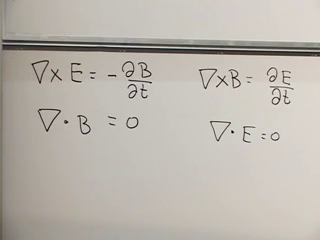
\includegraphics[width=0.76\textwidth]{lecture_58_figure_06.png}
\caption{四个真空麦克斯韦方程，其排列方式显示出电场与磁场之间的近似对称性。}
\lectureframe{00:27:30}
\end{figure}

电荷密度\(\rho\)最终将取代方程~\eqref{eq:gauss-e-vac}右端的零，电流密度\(\mathbf J\)将进入方程~\eqref{eq:ampere-vac}。我们暂时推迟这些项。无源方程以最少的杂乱揭示了变换结构和波动机制。

它们也使爱因斯坦的难题更加尖锐。一个跟随波运动的伽利略观察者会期望减去速度并测得较小的波速。然而，如果同样的麦克斯韦方程组在每个惯性系中都成立，那么每个观察者都会导出相同的单位波速。出路不是在不同参考系之间改变波动方程。而是使用洛伦兹变换，并把麦克斯韦方程组用变换规律已知的对象表示出来。

\section{电场与磁场作为一个张量}

电场和磁场组合成反对称场张量
\begin{equation}
F^{\mu\nu}=
\begin{pmatrix}
0   & -E_x & -E_y & -E_z\\
E_x & 0    & -B_z & B_y\\
E_y & B_z  & 0    & -B_x\\
E_z & -B_y & B_x  & 0
\end{pmatrix},
\label{eq:l0203-field-tensor}
\end{equation}
其中行和列的次序为\(t,x,y,z\)。反对称性，
\begin{equation}
F^{\mu\nu}=-F^{\nu\mu},
\end{equation}
迫使对角元为零，并由上半部分确定矩阵的下半部分。时间-空间元包含\(\mathbf E\)；纯空间元包含\(\mathbf B\)。

\begin{figure}[H]
\centering
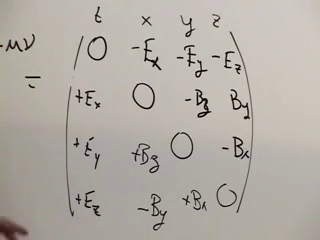
\includegraphics[width=0.58\textwidth]{lecture_58_figure_03.png}
\caption{完整的电磁场张量，包括其电的和磁的元。}
\lectureframe{00:32:05}
\end{figure}

\(F^{\mu\nu}\)的重要性不仅仅在于六个场分量能装进一个矩阵。在洛伦兹变换下，它作为二阶张量变换。因此，不同观察者测得的电场和磁场恰好以整个对象协调变换所需的方式混合。

还有第二个反对称张量，即对偶场张量\(\widetilde F^{\mu\nu}\)。在目前的约定下，它由方程~\eqref{eq:l0203-field-tensor}通过替换
\begin{equation}
\mathbf E\longmapsto-\mathbf B,
\qquad
\mathbf B\longmapsto\mathbf E.
\label{eq:dual-replacement}
\end{equation}
得到。因此
\begin{equation}
\widetilde F^{\mu\nu}=
\begin{pmatrix}
0    & B_x  & B_y  & B_z\\
-B_x & 0    & -E_z & E_y\\
-B_y & E_z  & 0    & -E_x\\
-B_z & -E_y & E_x  & 0
\end{pmatrix}.
\label{eq:dual-tensor}
\end{equation}
方程~\eqref{eq:dual-replacement}中的符号很重要。讲座先口头尝试交换，发现符号不匹配，并在完成矩阵之前加以修正。

\begin{figure}[H]
\centering
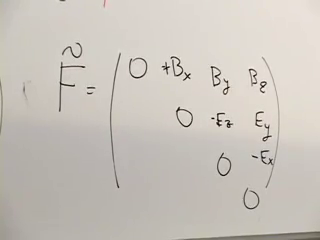
\includegraphics[width=0.58\textwidth]{lecture_58_figure_07.png}
\caption{通过以所需的符号交换电的和磁的元来组装对偶张量。}
\lectureframe{00:35:45}
\end{figure}

\section{协变的真空方程}

每个麦克斯韦方程都包含一个导数。从一个二阶张量出发并缩并一个导数指标后，剩下一个自由指标，因此自然的协变候选是
\begin{align}
\partial_\mu F^{\mu\nu}&=0,
\label{eq:maxwell-covariant-vac}\\
\partial_\mu\widetilde F^{\mu\nu}&=0.
\label{eq:maxwell-dual-vac}
\end{align}
对于\(\nu\)的每个固定值，方程~\eqref{eq:maxwell-covariant-vac}是一个方程。由于\(\nu\)可以是\(t,x,y,z\)，它打包了四个标量方程。方程~\eqref{eq:maxwell-dual-vac}打包了另外四个。这与原始列表中的两个矢量旋度方程和两个标量散度方程相符。

紧凑记号只有在能重现熟悉的方程时才有用。取\(\nu=z\)：
\begin{align}
\partial_\mu F^{\mu z}
&=\partial_tF^{tz}
  +\partial_xF^{xz}
  +\partial_yF^{yz}
  +\partial_zF^{zz}\\
&=-\partial_tE_z+\partial_xB_y-\partial_yB_x\\
&=-\partial_tE_z+
  \bigl(\boldsymbol\nabla\times\mathbf B\bigr)_z.
\end{align}
项\(F^{zz}\)因反对称性而消失。令结果为零，得到
\begin{equation}
\boldsymbol\nabla\times\mathbf B=\partial_t\mathbf E.
\end{equation}
的\(z\)分量。通过循环指标可得\(x\)和\(y\)分量。

\begin{figure}[H]
\centering
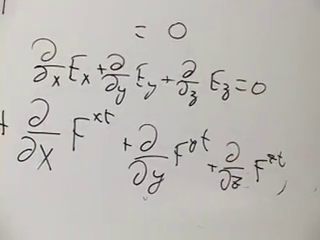
\includegraphics[width=0.76\textwidth]{lecture_58_figure_08.png}
\caption{协变场方程的分量展开；对角张量分量消失，其余项重构出麦克斯韦方程组。}
\lectureframe{00:43:30}
\end{figure}

现在取时间分量：
\begin{align}
\partial_\mu F^{\mu t}
&=\partial_tF^{tt}
  +\partial_xF^{xt}
  +\partial_yF^{yt}
  +\partial_zF^{zt}\\
&=\partial_xE_x+\partial_yE_y+\partial_zE_z\\
&=\boldsymbol\nabla\cdot\mathbf E.
\end{align}
因此它给出方程~\eqref{eq:gauss-e-vac}。对偶张量进行同样的检验得到
\(\boldsymbol\nabla\cdot\mathbf B=0\)和
\(\boldsymbol\nabla\times\mathbf E=-\partial_t\mathbf B\)。

这些紧凑方程现在已被确立，而不仅仅是猜测。它们的自由指标结构使它们成为四维矢量方程，因此洛伦兹变换改变其分量但不改变其形式。这正是真空麦克斯韦方程在每个惯性系中都相同的精确含义。

\section{从一阶方程到波}

麦克斯韦方程只包含一阶导数，而波动方程包含二阶导数。这一表面上的不匹配之所以得到解决，是因为麦克斯韦理论耦合了两个场。关于\(\mathbf E\)和\(\mathbf B\)的一对方程可以合并为关于任一单独场的二阶方程。

将方程~\eqref{eq:ampere-vac}对时间求导：
\begin{equation}
\partial_t^2\mathbf E
=\boldsymbol\nabla\times\partial_t\mathbf B.
\end{equation}
法拉第定律给出\(\mathbf B\)的时间导数，
\begin{equation}
\partial_t\mathbf B=-\boldsymbol\nabla\times\mathbf E,
\end{equation}
因此
\begin{equation}
\partial_t^2\mathbf E
=-\boldsymbol\nabla\times
  \bigl(\boldsymbol\nabla\times\mathbf E\bigr).
\label{eq:double-curl}
\end{equation}

黑板上的推导逐分量进行，而不是引用一个记忆中的恒等式。对于\(x\)分量，
\begin{align}
\bigl[\boldsymbol\nabla\times
(\boldsymbol\nabla\times\mathbf E)\bigr]_x
&=\partial_y(\boldsymbol\nabla\times\mathbf E)_z
 -\partial_z(\boldsymbol\nabla\times\mathbf E)_y\\
&=\partial_y(\partial_xE_y-\partial_yE_x)\\
&\quad-\partial_z(\partial_zE_x-\partial_xE_z)\\
&=\partial_x(\partial_yE_y+\partial_zE_z)
 -\partial_y^2E_x\\
&\quad-\partial_z^2E_x.
\end{align}
加减\(\partial_x^2E_x\)以显露出散度：
\begin{align}
\bigl[\boldsymbol\nabla\times
(\boldsymbol\nabla\times\mathbf E)\bigr]_x
&=\partial_x(\boldsymbol\nabla\cdot\mathbf E)
 -\nabla^2E_x.
\label{eq:double-curl-x}
\end{align}
在真空中\(\boldsymbol\nabla\cdot\mathbf E=0\)。结合方程~\eqref{eq:double-curl}和\eqref{eq:double-curl-x}得到
\begin{equation}
\left(\partial_t^2-\nabla^2\right)E_x=0.
\label{eq:ex-wave}
\end{equation}

\begin{figure}[H]
\centering
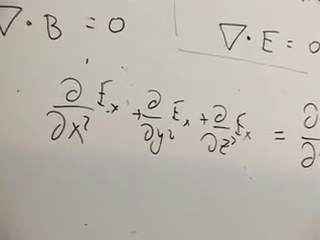
\includegraphics[width=0.72\textwidth]{lecture_58_figure_09.png}
\caption{分量计算得到\(E_x\)的波动方程。}
\lectureframe{00:57:10}
\end{figure}

同样的计算适用于\(E_y\)和\(E_z\)，类似的消元给出
\begin{equation}
\left(\partial_t^2-\nabla^2\right)\mathbf B=0.
\end{equation}
因此电场和磁场可以作为波在真空中传播。在此处使用的单位中，它们的速度为一，这意味着当恢复普通单位时速度为\(c\)。

\section{平面波及其偏振}

构造一个沿\(z\)正方向传播的简单波：
\begin{equation}
\mathbf E(z,t)
=\widehat{\mathbf x}\,E_0
  \cos\!\bigl(k(z-t)\bigr).
\label{eq:plane-e}
\end{equation}
其波形沿\(z\)平移而不改变形状。由于电场沿\(x\)轴指向，该波在\(x\)方向上为线偏振。我们选择\(E_y=0\)只是为了保持例子简单；本可以包含第二个横向偏振。

纵向分量并非同样自由。由于波只依赖于\(z\)和\(t\)，
\begin{equation}
\boldsymbol\nabla\cdot\mathbf E
=\partial_zE_z=0.
\end{equation}
因此\(E_z\)可以是常数，但不能包含变化的波形。均匀背景场可以独立地叠加或移除；它不是传播辐射的一部分。波本身是横波：
\begin{equation}
\mathbf E_{\mathrm{wave}}\cdot\widehat{\mathbf z}=0.
\end{equation}

法拉第定律确定磁场。对于方程~\eqref{eq:plane-e}，\(\boldsymbol\nabla\times\mathbf E\)的唯一非零分量是\(y\)分量，
\begin{equation}
(\boldsymbol\nabla\times\mathbf E)_y=\partial_zE_x.
\end{equation}
因此\(\partial_t\mathbf B\)沿\(y\)指向，一个相容的选择是
\begin{equation}
\mathbf B(z,t)
=\widehat{\mathbf y}\,E_0
  \cos\!\bigl(k(z-t)\bigr).
\label{eq:plane-b}
\end{equation}
在这些单位中，电场和磁场的振幅相等。它们的取向满足
\begin{equation}
\mathbf E\perp\mathbf B,
\qquad
\mathbf E\perp\widehat{\mathbf z},
\qquad
\mathbf B\perp\widehat{\mathbf z},
\qquad
\mathbf E\times\mathbf B\parallel\widehat{\mathbf z}.
\end{equation}

\begin{figure}[H]
\centering
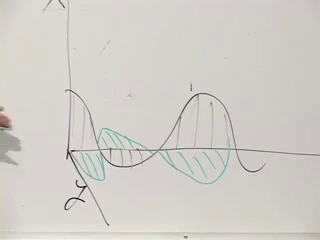
\includegraphics[width=0.70\textwidth]{lecture_58_figure_05.png}
\caption{横电磁波的完整黑板示意图：电场和磁场的振荡彼此垂直，且都垂直于传播方向。}
\lectureframe{01:05:25}
\end{figure}

\begin{figure}[H]
\centering
\scalebox{0.90}{%
\begin{tikzpicture}[x=1cm,y=1cm,>=Latex]
  \draw[->,thick] (0,0) -- (8.2,0) node[right] {$z$};
  \draw[->,thick] (0,-1.6) -- (0,1.7) node[above] {$x$};
  \draw[->,thick] (0,0) -- (-1.15,-0.8) node[below left] {$y$};
  \draw[blue!70!black,thick,domain=0:7.5,samples=120]
    plot (\x,{0.95*sin(90*\x)});
  \foreach \z/\s in {0.8/1,2.8/-1,4.8/1,6.8/-1}{
    \draw[->,green!45!black,thick]
      (\z,0) -- ++({-0.55*\s},{-0.38*\s});
  }
  \node[blue!70!black] at (6.9,1.25) {$\mathbf E$};
  \node[green!45!black] at (5.2,-1.05) {$\mathbf B$};
  \draw[->,very thick] (6.2,1.55) -- (7.7,1.55)
    node[midway,above] {propagation};
\end{tikzpicture}
}
\caption{场\(\mathbf E\)和\(\mathbf B\)彼此垂直，且都垂直于传播方向。}
\end{figure}

这就是光以及真空中所有电磁辐射的特征。由于产生该波的方程是洛伦兹协变的，另一个惯性观察者同样会描述一个以\(c\)运动的电磁波，具有横向的电场和磁场。

\section{电荷密度与电流密度}

现在恢复此前暂时搁置的源。当许多带电粒子占据一个区域时，将它们粗粒化为连续电荷密度是方便的
\begin{equation}
\rho(\mathbf x,t)=\frac{dQ}{dV}.
\end{equation}
这种近似就像把水当作连续流体来处理，尽管水由分子组成。正电荷与负电荷以相反的符号贡献，因此\(\rho\)是单位体积的净电荷。

所选区域\(V\)内的电荷为
\begin{equation}
Q_V(t)=\int_V\rho(\mathbf x,t)\,dV.
\label{eq:charge-volume}
\end{equation}
密度可以随位置和时间变化。一堆电荷可以从某点移走，从而改变该处的局域密度。然而，它不能以任意方式变化。自然界守恒电荷。

仅全局守恒太弱。它会允许电荷在同一瞬间从地球消失并在火星出现，而总量保持不变。更强的陈述是局域的：电荷只能通过中间空间中的流动离开一处并到达另一处。

为了描述这种流动，取一个无穷小有向面元
\begin{equation}
d\boldsymbol\sigma=\widehat{\mathbf n}\,d\sigma.
\end{equation}
其大小是面积，其方向垂直于表面。电流密度\(\mathbf J\)的定义使得单位时间穿过该面元的电荷为
\begin{equation}
\frac{dQ}{dt}=\mathbf J\cdot d\boldsymbol\sigma.
\label{eq:current-flux-element}
\end{equation}
\(\mathbf J\)的大小是单位面积单位时间的电荷，其方向是正电荷流动的方向。

\begin{figure}[H]
\centering
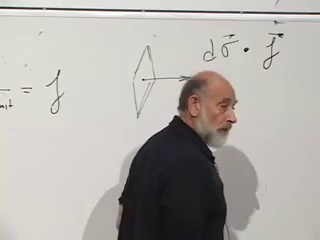
\includegraphics[width=0.64\textwidth]{lecture_58_figure_10.png}
\caption{有向面元与通量因子\(d\boldsymbol\sigma\cdot\mathbf J\)。}
\lectureframe{01:18:15}
\end{figure}

点积选出垂直于表面的分量。与表面相切的电流不穿过任何一侧，贡献为零。平行于法线的电流在大小固定时给出最大通量。导线电流是一种特殊情况，但\(\mathbf J\)也可以描述穿过薄片或在整个三维空间中流动的电荷。

\section{局域守恒与连续性方程}

固定空间中的一个区域\(V\)，并将其闭合边界\(\partial V\)的每个面元取为外法向。如果存在净向外的电流，则内部电荷减少：
\begin{equation}
\frac{dQ_V}{dt}
=-\oint_{\partial V}\mathbf J\cdot d\boldsymbol\sigma.
\label{eq:integral-conservation}
\end{equation}
负号是物理的而非约定的：正的向外通量从该区域移走正电荷。利用方程~\eqref{eq:charge-volume}，
\begin{equation}
\int_V\partial_t\rho\,dV
=-\oint_{\partial V}\mathbf J\cdot d\boldsymbol\sigma.
\label{eq:integral-continuity-one}
\end{equation}

\begin{figure}[H]
\centering
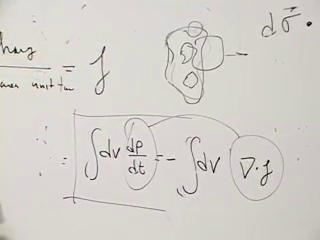
\includegraphics[width=0.72\textwidth]{lecture_58_figure_11.png}
\caption{将表面通量转化为体积陈述后的固定区域守恒定律。}
\lectureframe{01:29:00}
\end{figure}

高斯定理，也称为散度定理，将穿过闭合曲面的通量与其内部的散度联系起来：
\begin{equation}
\oint_{\partial V}\mathbf A\cdot d\boldsymbol\sigma
=\int_V\boldsymbol\nabla\cdot\mathbf A\,dV.
\label{eq:divergence-theorem}
\end{equation}
可以想象隐藏的管道在容器内部的各点注入水。散度衡量水从管端冒出的局域速率；面积分衡量离开容器的总水量。内部作为向外流动而被创造出来的东西，最终必须穿过边界。

将方程~\eqref{eq:divergence-theorem}应用于\(\mathbf J\)得到
\begin{equation}
\int_V
\left(\partial_t\rho+\boldsymbol\nabla\cdot\mathbf J\right)dV=0.
\end{equation}
此关系对每一个可能的区域\(V\)都成立。因此被积函数必须逐点为零：
\begin{equation}
\boxed{\partial_t\rho+\boldsymbol\nabla\cdot\mathbf J=0.}
\label{eq:continuity-three}
\end{equation}

\begin{figure}[H]
\centering
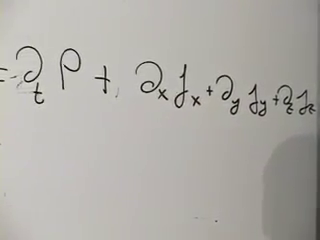
\includegraphics[width=0.72\textwidth]{lecture_58_figure_12.png}
\caption{逐分量写出的局域连续性方程。}
\lectureframe{01:29:50}
\end{figure}

方程~\eqref{eq:continuity-three}恰好说明了局域守恒所要求的内容。如果电荷密度在某点或小区域内减少，电流必须从该处向外发散。如果电流向内汇聚，电荷密度就增加。

密度和电流自然地组成四维电流
\begin{equation}
J^\mu=(\rho,J_x,J_y,J_z)
\label{eq:four-current}
\end{equation}
在\(c=1\)单位下。连续性方程变为洛伦兹标量方程
\begin{equation}
\partial_\mu J^\mu=0.
\label{eq:continuity-four}
\end{equation}
相对论性分布的流动应当像单个粒子的四维速度一样按四维矢量变换。方程~\eqref{eq:continuity-four}使局域电荷守恒在每个惯性系中都成立。

\section{有源的麦克斯韦方程组}

恢复电荷和电流后得到
\begin{align}
\boldsymbol\nabla\cdot\mathbf E&=\rho,
\label{eq:gauss-e-source}\\
\boldsymbol\nabla\cdot\mathbf B&=0,\\
\boldsymbol\nabla\times\mathbf E&=-\partial_t\mathbf B,\\
\boldsymbol\nabla\times\mathbf B&=\partial_t\mathbf E+\mathbf J.
\label{eq:ampere-source}
\end{align}
涉及电性源的方程合并为
\begin{equation}
\boxed{\partial_\mu F^{\mu\nu}=J^\nu,}
\label{eq:maxwell-source-covariant}
\end{equation}
而无源的磁方程对仍为
\begin{equation}
\boxed{\partial_\mu\widetilde F^{\mu\nu}=0.}
\label{eq:maxwell-dual-source}
\end{equation}

\begin{figure}[H]
\centering
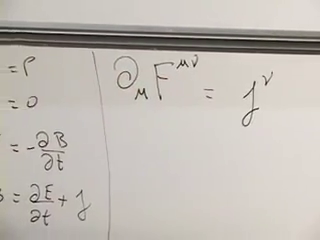
\includegraphics[width=0.78\textwidth]{lecture_58_figure_13.png}
\caption{有源麦克斯韦方程组及其协变形式\(\partial_\mu F^{\mu\nu}=J^\nu\)。}
\lectureframe{01:34:00}
\end{figure}

方程~\eqref{eq:maxwell-source-covariant}的时间分量读作
\begin{equation}
\partial_\mu F^{\mu t}=J^t=\rho,
\end{equation}
而已经完成的分量计算将其左侧化为
\(\boldsymbol\nabla\cdot\mathbf E\)。三个空间分量重现
\(\boldsymbol\nabla\times\mathbf B=\partial_t\mathbf E+\mathbf J\)。

还有一个有用的一致性检验。将\(\partial_\nu\)作用于
方程~\eqref{eq:maxwell-source-covariant}得到
\begin{equation}
\partial_\nu J^\nu
=\partial_\nu\partial_\mu F^{\mu\nu}=0,
\end{equation}
因为两个导数在\(\mu\leftrightarrow\nu\)下对称，而\(F^{\mu\nu}\)是反对称的。\editorialnote{这个简短的一致性检验由协变方程得出，并明确说明了为什么有源麦克斯韦方程组自动满足连续性方程。}

互反结构至此完备。张量力定律
\(f^\mu=qF^\mu{}_\nu u^\nu\)描述了场如何作用于电荷，而
方程~\eqref{eq:maxwell-source-covariant}描述了电荷与电流如何产生场。二者均为张量方程。在真空中，同一组场方程给出以\(c\)传播的横波。因此，洛伦兹协变性与电磁波方程在当初促使这一构造的关节点上汇合：每个惯性观测者都得到相同的电磁学定律和相同的光速。
\chapter{固有时、时间膨胀与长度收缩}

我们将经常选取光速为$c=1$的单位制。在这种单位制下，一年的时间与一光年的距离可以直接比较，公式也更容易阅读。只要$c$在物理上起作用，我们就把它放回去。量纲分析足以确定它的位置。

\section{伽利略时空网格}

从爱因斯坦之前静止参考系与沿$x$轴以速度$v$运动的列车之间的关系出发：
\begin{align}
x' &= x-vt, & t'&=t.
\label{eq:l4-galilean}
\end{align}
第二个方程包含了牛顿关于普适时间的假设。即使空间原点彼此相对运动，每个观测者都使用相同的同时性切片。

假设不带撇的观测者站在轨道旁，带撇的观测者乘在列车上。列车原点满足$x'=0$，因此它在不带撇坐标中的世界线为
\begin{equation}
x=vt.
\end{equation}
这条倾斜的直线就是$t'$轴。相反，$t'=t$表明所有常$t'$的直线与常$t$的直线是相同的水平线。

\begin{figure}[H]
\centering
\includegraphics[width=0.72\textwidth]{lecture_04_figure_02.png}
\caption{伽利略变换与初始$t$-$x$网格。运动的原点将描出$x=vt$，而两个参考系保持共同的等时线。}
\lectureframe{00:03:06}
\end{figure}

对式~\eqref{eq:l4-galilean}求解不带撇的坐标，得到
\begin{align}
x&=x'+vt'=x'+vt, & t&=t'.
\end{align}
逆变换具有相同的形式，只是$v$被替换为$-v$。如果列车相对于车站向前运动，那么车站相对于列车向后运动。这种互易性在狭义相对论中仍然成立，但普适时间不再成立。

\section{洛伦兹修正}

伽利略变换无法使光速在每个惯性系中都相同。修正后的关系式，首先在$c=1$单位下为
\begin{align}
x'&=\frac{x-vt}{\sqrt{1-v^2}}, &
t'&=\frac{t-vx}{\sqrt{1-v^2}}.
\label{eq:l4-lorentz-natural}
\end{align}
恢复普通单位后得到
\begin{align}
x'&=\frac{x-vt}{\sqrt{1-v^2/c^2}}, &
t'&=\frac{t-vx/c^2}{\sqrt{1-v^2/c^2}}.
\label{eq:l4-lorentz-c}
\end{align}

\begin{figure}[H]
\centering
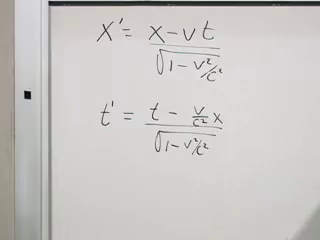
\includegraphics[width=0.74\textwidth]{lecture_04_figure_05.png}
\caption{恢复了$c$因子的洛伦兹变换。}
\lectureframe{00:09:10}
\end{figure}

对于$v\ll c$，在使用牛顿力学的场合中，$v^2/c^2$和$vx/c^2$都很小。此时式~\eqref{eq:l4-lorentz-c}约化为伽利略结果。相对论并未抛弃牛顿运动学；它确定了牛顿运动学的有效范围。

当$v=c$时，分母为零。一个惯性系不能相对于另一个惯性系以光速运动。远低于该极限时修正很小，但接近它时，$x$与$t$的混合变得不可避免。

运动是沿$x$选取的，因此横向坐标不变：
\begin{equation}
y'=y,\qquad z'=z.
\end{equation}
理解这一点的一种方法是，在列车和站台上放置相同的横向米尺。一个在两个参考系正中间运动的观测者看到两根尺以大小相等、方向相反的速度接近。这个设置没有任何特征能使一根横向尺比另一根短。

\section{沿光锥的洛伦兹变换}

有一种几何方式来解读式~\eqref{eq:l4-lorentz-natural}。将其两个方程相加：
\begin{align}
t'+x'
&=\frac{(t-vx)+(x-vt)}{\sqrt{1-v^2}}\\
&=(t+x)\frac{1-v}{\sqrt{1-v^2}}\\
&=(t+x)\sqrt{\frac{1-v}{1+v}}.
\label{eq:l4-null-plus}
\end{align}
以互补的顺序相减：
\begin{align}
t'-x'
&=\frac{(t-vx)-(x-vt)}{\sqrt{1-v^2}}\\
&=(t-x)\frac{1+v}{\sqrt{1-v^2}}\\
&=(t-x)\sqrt{\frac{1+v}{1-v}}.
\label{eq:l4-null-minus}
\end{align}

\begin{figure}[H]
\centering
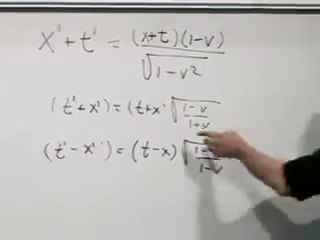
\includegraphics[width=0.75\textwidth]{lecture_04_figure_06.png}
\caption{用零组合$t+x$和$t-x$重写的洛伦兹变换。它们的比例因子互为倒数。}
\lectureframe{00:18:45}
\end{figure}

组合$t+x$和$t-x$是沿两个$45^\circ$类光方向的坐标。一个推进会压缩其中一个方向，并以倒数因子拉伸另一个方向。它不会使其中任何一个方向偏离$45^\circ$。因此光线仍然是光线，这就是光速不变性的时空图景。

\begin{classroomqa}
\audiencequestion{正中间的观测者看到一个对称的实验，但这如何为列车和站台上的观测者确立结果？\lecturetimestamp{00:20:48}}
\lecturerresponse{这里还使用了另一个事实：事件的重合是不变的。如果两根尺的端点相遇，那次相遇就是一个时空事件。每个惯性观测者可以给它赋予不同的坐标，但没有人能把一次重合分成两个不同的位置。在相应端点相遇处发出的闪光使这些事件在操作上可被探测。正中间参考系的对称性以及两个端点重合的不变性，确立了横向长度一致。}
\end{classroomqa}

\begin{classroomqa}
\audiencequestion{代表中间参考系的骑自行车者是否必须物理上位于两根杆的中点？\lecturetimestamp{00:22:25}}
\lecturerresponse{不。参考系是一整套由观察者和时钟构成的网络，而不是位于某一位置的一只眼睛。骑自行车者可以在稍后接收到端点发出的闪光，并推断它们源自何处。重要的是每个发射事件在时空中的位置，而不是光最终在哪里被接收到。}
\end{classroomqa}

相继速度的合成是同一变换的另一个推论，但有意留到下一讲。当前的任务是确定运动时钟所测量的不变量。

\section{不变间隔}

对于普通笛卡尔坐标轴的旋转，量$x^2+y^2$保持不变。洛伦兹变换保持的是另一个二次型。由式~\eqref{eq:l4-lorentz-natural}，
\begin{align}
t'^2-x'^2
&=\frac{(t-vx)^2-(x-vt)^2}{1-v^2}\\
&=\frac{t^2-2vtx+v^2x^2-x^2+2vtx-v^2t^2}{1-v^2}\\
&=t^2-x^2.
\label{eq:l4-interval}
\end{align}
交叉项相消，剩余的分子含有公因子$1-v^2$。

\begin{figure}[H]
\centering
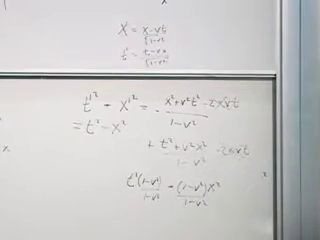
\includegraphics[width=0.76\textwidth]{lecture_04_figure_07.png}
\caption{黑板上对$t'^2-x'^2=t^2-x^2$的推导。}
\lectureframe{00:33:15}
\end{figure}

在三维空间中，不变量为
\begin{equation}
t'^2-x'^2-y'^2-z'^2=t^2-x^2-y^2-z^2
\end{equation}
以$c=1$为单位。更一般地，对于两个事件，我们使用坐标差：
\begin{equation}
\Delta s^2
=c^2\Delta t^2-\Delta x^2-\Delta y^2-\Delta z^2.
\label{eq:l4-spacetime-interval}
\end{equation}
每个惯性观察者都同意这个数，尽管他们对其中的时间项和空间项分别并不一致。

\section{固有时与运动时钟}

想象一个由静止观察者组成的格点，他们的时钟已通过交换光信号同步。他们的读数定义了坐标时间$t$。现在让一只手表穿过这个格点。它自身的读数沿着其世界线跟随这只手表；该读数就是固有时。

对于两个类时分离的事件，定义
\begin{equation}
c^2\Delta\tau^2
=c^2\Delta t^2-\Delta x^2-\Delta y^2-\Delta z^2.
\label{eq:l4-proper-time}
\end{equation}
在一维空间中，当$c=1$时，这简单地就是
\begin{equation}
\Delta\tau=\sqrt{\Delta t^2-\Delta x^2}.
\end{equation}
平方根与普通距离的公式类似，但负号改变了几何。

有三种情况：
\begin{align}
\Delta t^2-\Delta x^2 &>0 &&\text{timelike},\\
\Delta t^2-\Delta x^2 &=0 &&\text{lightlike},\\
\Delta t^2-\Delta x^2 &<0 &&\text{spacelike}.
\end{align}
在光锥内部，固有时为实数。在光锥上，即$x=\pm t$处，即使事件不必重合，固有时也为零。光线恰好可以连接这样的事件。在光锥外部，间隔是类空的；用实固有距离$\sqrt{\Delta x^2-\Delta t^2}$来描述它比用虚时钟时间更好。

\begin{figure}[H]
\centering
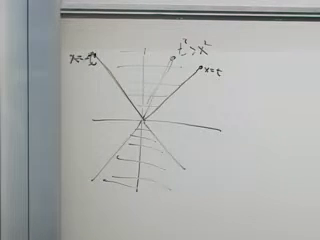
\includegraphics[width=0.73\textwidth]{lecture_04_figure_08.png}

\vspace{0.8em}

\begin{tikzpicture}[x=1.0cm,y=1.0cm]
\draw[->] (-3.3,0) -- (3.3,0) node[right] {$x$};
\draw[->] (0,-0.4) -- (0,4.0) node[above] {$t$};
\draw[thick] (0,0) -- (3.0,3.0) node[above right] {$x=t$};
\draw[thick] (0,0) -- (-3.0,3.0) node[above left] {$x=-t$};
\node at (0,2.0) {timelike};
\node at (2.25,1.05) {spacelike};
\node at (-2.25,1.05) {spacelike};
\end{tikzpicture}
\caption{黑板上的光锥以及对类时、类光、类空间隔的清晰分类。}
\lectureframe{00:38:40}
\end{figure}

为什么式~\eqref{eq:l4-proper-time}等于时钟读数？对于静止的时钟，$\Delta x=0$，所以$\Delta\tau=\Delta t$。对于匀速运动的时钟，选择该时钟在其中静止的带撇参考系。在那里$\Delta x'=0$，而不变性给出
\begin{equation}
\Delta\tau
=\sqrt{\Delta t'^2-\Delta x'^2}
=\Delta t'.
\end{equation}
因此运动时钟记录的就是固有时。

\begin{classroomqa}
\audiencequestion{``事件之间的间隔''和``时钟的读数''是否被用作同一事物的两个名称？
\lecturetimestamp{00:44:49}}
\lecturerresponse{当一个理想时钟从一个事件惯性运动到另一个事件时，它们重合。不变间隔是一个几何量；共动时钟的端点读数之差是它的物理测量。静止的坐标时钟通常记录不同的坐标时间间隔。}
\end{classroomqa}

\section{时间膨胀与同时性}

考虑运动参考系的原点。它的世界线满足
\begin{equation}
x'=0,\qquad x=vt.
\end{equation}
同一条斜线既是运动时钟的路径，也是$t'$轴。

\begin{figure}[H]
\centering
\includegraphics[width=0.72\textwidth]{lecture_04_figure_03.png}
\caption{运动原点：$x=vt$、$x'=0$和$t'$轴是同一条世界线的三种描述。}
\lectureframe{00:48:18}
\end{figure}

对共同原点和该世界线上稍后一点应用不变间隔：
\begin{align}
t'^2-x'^2&=t^2-x^2,\\
t'^2&=t^2-v^2t^2,\\
t'&=t\sqrt{1-v^2}.
\label{eq:l4-time-dilation-natural}
\end{align}
恢复$c$后，
\begin{equation}
\Delta\tau=\Delta t\sqrt{1-\frac{v^2}{c^2}}
=\frac{\Delta t}{\gamma},
\qquad
\gamma=\frac{1}{\sqrt{1-v^2/c^2}}.
\label{eq:l4-time-dilation}
\end{equation}

\begin{figure}[H]
\centering
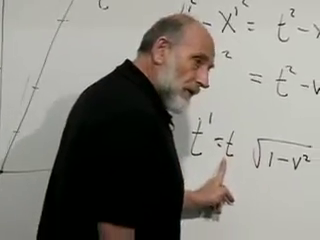
\includegraphics[width=0.73\textwidth]{lecture_04_figure_09.png}
\caption{黑板上的时间膨胀结果：运动时钟累积$t'=t\sqrt{1-v^2}$，单位取$c=1$。}
\lectureframe{00:50:45}
\end{figure}

静止观察者说运动时钟走得慢。互易性要求运动观察者对静止时钟说同样的话。这并不矛盾，因为两种描述比较的是不同的远距事件对。

确实，式~\eqref{eq:l4-lorentz-natural}中$t'$取常数值满足
\begin{equation}
t-vx=\text{constant}.
\label{eq:l4-simultaneity}
\end{equation}
运动观察者的同时线相对于水平线$t=\text{constant}$是倾斜的。每个观察者把不同的一组远距时钟读数称为同时的。一旦保持这种差异可见，时钟的相互变慢就是一致的。

\begin{figure}[H]
\centering
\begin{tikzpicture}[x=1cm,y=1cm]
\draw[->] (0,0) -- (0,4.2) node[above] {$t$};
\draw[->] (0,0) -- (5.2,0) node[right] {$x$};
\draw[thick,->] (0,0) -- (2.4,3.8) node[above] {$x'=0$};
\draw[dashed] (0,2.8) -- (4.8,2.8)
  node[right] {$t=\mathrm{const}$};
\draw[thick] (0.15,1.05) -- (4.7,2.35)
  node[right] {$t'=\mathrm{const}$};
\draw[thick] (3.4,0) -- (3.4,3.8);
\fill (3.4,2.8) circle (0.045);
\fill (3.4,1.98) circle (0.045);
\end{tikzpicture}
\caption{互易时间膨胀比较的是不同同时切片上的时钟读数。}
\end{figure}

\section{孪生路径}

两个双胞胎从同一事件出发。一个留在$x=0$处。另一个以速度$v$向外运动，然后反向并以相同速度返回。当他们重逢时，他们比较每一个可以作为时钟的物理过程：手表、心跳、新陈代谢或衰老本身。

设每一半旅程在家的参考系中花费坐标时间$T$。留在家中的双胞胎的固有时为
\begin{equation}
\tau_{\mathrm{home}}=2T.
\end{equation}
转向事件具有坐标$(vT,T)$。因此第一段旅行贡献
\begin{align}
\tau_{\mathrm{leg}}
&=\sqrt{T^2-v^2T^2}
=T\sqrt{1-v^2}.
\end{align}
返回段贡献相同的量，因此
\begin{equation}
\tau_{\mathrm{travel}}=2T\sqrt{1-v^2}<2T.
\label{eq:l4-twin}
\end{equation}

\begin{figure}[H]
\centering
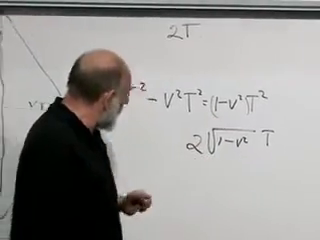
\includegraphics[width=0.73\textwidth]{lecture_04_figure_10.png}

\vspace{0.8em}

\begin{tikzpicture}[x=1.1cm,y=1cm]
\draw[->] (-0.2,0) -- (3.4,0) node[right] {$x$};
\draw[->] (0,-0.1) -- (0,4.4) node[above] {$t$};
\draw[very thick] (0,0) -- (0,4);
\draw[very thick] (0,0) -- (2.2,2) -- (0,4);
\draw[dashed] (0,2) -- (2.2,2);
\node[left] at (0,2) {$T$};
\node[left] at (0,4) {$2T$};
\node[below right] at (1.1,1.0) {$v$};
\node[above right] at (1.1,3.0) {$-v$};
\end{tikzpicture}
\caption{留在家中的世界线和两段旅行。它们的固有时不同，因为它们是时空中的不同路径。}
\lectureframe{00:59:35}
\end{figure}

年龄不等并不矛盾。旅行路径包含一个转向，并且与直线在家的路径之间不存在单一惯性系对称性的关系。在普通欧几里得几何中，两点之间的直线路线和折线路线也有不同的长度。闵可夫斯基几何反转了哪条路径具有更大间隔，但比较仍然是几何的。

\section{加速度与理想时钟}

\begin{classroomqa}
\audiencequestion{在转向处物理情况不同，旅行者加速。这是否使时钟计算失效？
\lecturetimestamp{01:02:19}}
\lecturerresponse{加速度是真实的，并有助于识别不对称性；不应将其辩解掉。尖锐的拐角只是理想化的画法，可以圆滑化为有限的转向。进一步的物理假设是，一个足够小、构造良好的时钟对适度的加速度不敏感，并继续记录固有时。一个大或脆弱的时钟可能变形或损坏，但那是机制的缺陷，而不是时空间隔的缺陷。}
\end{classroomqa}

这个理想时钟假设并非仅从洛伦兹变换推导出来。它通过实际时钟机制的行为来检验。原子比横跨数百英里的时钟要好得多的近似，因为紧凑的机制在加速度或引力下更难变形。仅仅援引广义相对论的名字并不能消除这个物理问题；人们仍然必须知道所选机制如何响应其环境。

\begin{classroomqa}
\audiencequestion{能否将加速轨迹分解为短间隔，使得惯性分析在这些间隔上仍然有效？\lecturetimestamp{01:09:08}}
\lecturerresponse{可以。将曲线分成短的、近似直线的段，计算每一段上的固有时，然后将结果相加。这是用许多小线段求普通曲线长度的时空类比。在连续极限下，
\[
\tau=\int \sqrt{1-\frac{v(t)^2}{c^2}}\,dt,
\]
对于在惯性坐标系中描述的平直时空中的运动。}
\end{classroomqa}

\section{双胞胎看到什么}

最终的时钟读数可以通过发送光脉冲来操作化。在两条世界线上标记一秒的固有时间隔，并让每个双胞胎在每个标记处发出一个脉冲。在外出段，从另一个双胞胎接收到的脉冲被拉开。在返回段，它们成束到达。这是直接在时空图上表达的爱因斯坦相对论多普勒效应。

\begin{figure}[H]
\centering
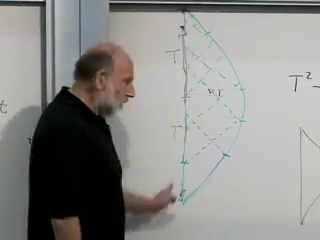
\includegraphics[width=0.73\textwidth]{lecture_04_figure_11.png}
\caption{在家和旅行世界线之间交换的光信号。外出段稀疏的到达和返回段压缩的到达解释了每一个发出的脉冲。}
\lectureframe{01:12:55}
\end{figure}

故事中没有参考系消失。每个观察者最终都会接收到对方发出的所有脉冲，但它们的接收率取决于相对运动。对于两条路径，外出的红移和返回的蓝移不是等持续时间效应，因此计数所有接收到的脉冲与固有时比较一致。

\begin{classroomqa}
\audiencequestion{如果返回的旅行者接收到蓝移的光，旅行者能否收集到比光源发出的更多的能量？
\lecturetimestamp{01:13:50}}
\lecturerresponse{这个问题需要能量的相对论定义和参考系依赖性，而这些尚未展开。这是合理的，但仅凭坐标和脉冲计数不足以解决能量记账，尤其是对于加速观察者。因此答案应推迟，而不是猜测。}
\end{classroomqa}

\section{一个闭合的空间方向}

\begin{classroomqa}
\audiencequestion{假设有一个空间方向是紧致的。一个孪生子能否沿它匀速运动，回到出发点，并且完全避免加速？那么又是什么区分了这对孪生子？\lecturetimestamp{01:15:14}}
\lecturerresponse{空间应当被内在地想象为一个圆柱面，而不是一张弯曲嵌入更大空间中的薄片；这里不必存在径向加速度。然而，返回的观测者会遇到这样一个整体事实：相同的地点会重复出现。这表明存在一种不对称性，但要给出完整答案，需要对带有空间认同的狭义相对论作细致处理。这个问题在此留作开放，而不是即兴作答。}
\end{classroomqa}

\begin{figure}[H]
\centering
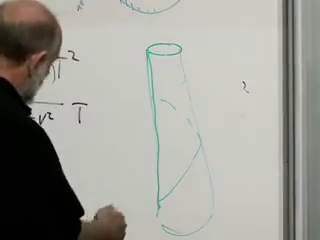
\includegraphics[width=0.72\textwidth]{lecture_04_figure_04.png}

\vspace{0.8em}

\begin{tikzpicture}[x=1cm,y=1cm]
\draw[thick] (0,0) ellipse (1.3 and 0.35);
\draw[thick] (-1.3,0) -- (-1.3,-3.1);
\draw[thick] (1.3,0) -- (1.3,-3.1);
\draw[thick] (0,-3.1) ellipse (1.3 and 0.35);
\draw[->,very thick] (0.0,0.38) arc (90:-210:1.38 and 0.42);
\node[right] at (1.65,-1.5) {compact spatial direction};
\end{tikzpicture}
\caption{黑板上所画的紧致空间问题，配有一个干净的内禀圆柱面。这是一个关于整体认同的问题，而不是关于绕着一个嵌入额外径向维度的圆柱面运动的问题。}
\lectureframe{01:17:56}
\end{figure}

\section{长度是在同时性切片上测量的}

对于狭义相对论问题，首先要画出时空图。取一根在未加撇系中静止的米尺，其端点位于$x=0$和$x=1$。随着时间流逝，两个端点描出竖直的世界线。这根尺在它们之间扫出一条带状区域。

运动的观测者必须在运动时间$t'$的同一个值上测量两个端点。由式~\eqref{eq:l4-simultaneity}，过原点且满足$t'=0$的切片在$c=1$单位下满足
\begin{equation}
t=vx
\end{equation}
它与右端点$x=1$相交于$t=v$。

\begin{figure}[H]
\centering
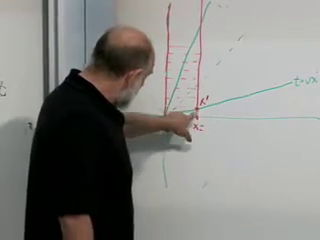
\includegraphics[width=0.73\textwidth]{lecture_04_figure_12.png}

\vspace{0.8em}

\begin{tikzpicture}[x=1.55cm,y=1.15cm]
\draw[->] (-0.5,0) -- (3.1,0) node[right] {$x$};
\draw[->] (0,0) -- (0,3.8) node[above] {$t$};
\draw[very thick,red] (0,0) -- (0,3.3);
\draw[very thick,red] (2.15,0) -- (2.15,3.3);
\fill[red!12] (0,0) rectangle (2.15,3.3);
\draw[very thick,green!50!black] (0,0) -- (1.2,3.1)
  node[above] {$x=vt$};
\draw[very thick,blue] (0,0) -- (2.15,1.15)
  node[right] {$t'=0$};
\fill (2.15,1.15) circle (0.045);
\node[right] at (2.22,1.35) {$(x,t)=(1,v)$};
\node[below] at (2.15,0) {$1$};
\end{tikzpicture}
\caption{一根静止的杆扫出一条时空带状区域。运动观测者所测的长度，是其端点在一个$t'=\mathrm{const}$切片上的间隔。}
\lectureframe{01:24:20}
\end{figure}

所选端点间隔是类空的，因此使用不变量的正空间形式：
\begin{equation}
x'^2-t'^2=x^2-t^2.
\end{equation}
在所选端点处，$t'=0$，$x=1$，且$t=v$。因此
\begin{align}
x'^2&=1-v^2,\\
x'&=\sqrt{1-v^2}.
\end{align}
于是，静长度$L$在运动系中被测得为
\begin{equation}
L'=L\sqrt{1-v^2/c^2}=\frac{L}{\gamma}.
\label{eq:l4-length-contraction}
\end{equation}

\begin{figure}[H]
\centering
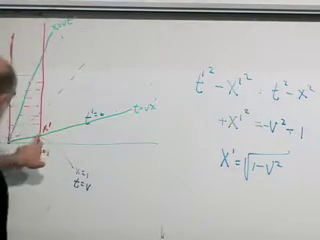
\includegraphics[width=0.76\textwidth]{lecture_04_figure_13.png}
\caption{完整的长度收缩作图以及单位静长度对应的黑板结果$x'=\sqrt{1-v^2}$。}
\lectureframe{01:28:10}
\end{figure}

相反的陈述同样成立：站台观测者赋予列车纵向米尺的长度更短。两位观测者又一次选择了不同的同时端点事件，因此这种互易性并不矛盾。

\section{结尾的问题}

\begin{classroomqa}
\audiencequestion{除了光之外，还有什么以光速传播？特别是引力呢？\lecturetimestamp{01:29:29}}
\lecturerresponse{广义相对论预言引力波以$c$传播。在这次讲座之时，证据间接来自双脉冲星等系统；引力波尚未被直接探测到。\editorialnote{在这次2006讲座之后，实验状况发生了变化。LIGO于2015年直接探测到GW150914，而对GW170817及其电磁对应体的联合观测于2017年表明，引力与光的传播速度在$10^{15}$分之几的精度内一致。参见\url{https://ligo.org/detections/gw150914/}和
\url{https://doi.org/10.1103/PhysRevLett.119.251302}。}}
\end{classroomqa}

\begin{classroomqa}
\audiencequestion{一名宇航员能否在比以光年表示的该距离更短的固有时内穿越许多光年的距离？那是否意味着运动得比光还快？\lecturetimestamp{01:30:38}}
\lecturerresponse{宇航员的固有时为
$\sqrt{\Delta t^2-\Delta x^2}$，它小于坐标时$\Delta t$。在宇航员的惯性系中，恒星之间的距离发生了洛伦兹收缩。恒星以速度$-v$运动，并不比光快；只是需要穿越的收缩后距离更短。}
\end{classroomqa}

如果宇航员从静止开始并加速，那么描述会在一系列瞬时惯性系之间发生变化。在此期间，赋予恒星的距离可以改变。人们不能对整个加速历史施加一个固定的洛伦兹变换，但总固有时仍可通过沿世界线累加各贡献而得到。同样的陈述也适用于一个真实的孪生子：他发射、转向并减速，而不是以巡航速度出生。

\begin{classroomqa}
\audiencequestion{这些困惑是否源于把时间当作特殊的存在？我们是否必须称它为第四维？\lecturetimestamp{01:36:43}}
\lecturerresponse{不必从“时间是第四维”这一口号出发。洛伦兹变换本身就迫使空间与时间相互混合，而间隔$t^2-x^2-y^2-z^2$则将它们视为同一几何的组成部分，只是时间与空间带有不同的符号。在低速下，这种混合变得可以忽略，熟悉的牛顿直觉重新出现。然而在相对论速度下，空间与时间不能被视为从根本上彼此脱耦。}
\end{classroomqa}

因此，时间膨胀、长度收缩、双生子比较以及缩短的旅行时间并非各自独立的把戏。它们都源自三个习惯：确定被比较的事件，画出它们的时空几何，并利用不变间隔。
\chapter{火球、参考系与四维矢量}

我们从高能碰撞讨论中遗留的一个问题开始。两个重核的碰撞产生的是一个剧烈变化的对象，而不是一个宁静的天文黑洞。那么，用视界来描述这种碰撞究竟意味着什么？答案将经由强耦合物质的五维图像、一组关于加速器的实际问题，最终回到狭义相对论的几何。到结束时，速度和动量已成为四维矢量，而能量则在动量的三个分量旁边占据了自己的位置。

\section{第五维中的火球}

\begin{classroomqa}
\audiencequestion{碰撞中产生的对象是不稳定的，并且会改变形状。这样一个复杂的对象怎么能被称为黑洞呢？}
\lecturerresponse{设想第五个空间方向在地板与天花板之间延伸。该方向上的引力将激发态拉向地板。碰撞在那里沉积了一团炽热的能量块；这团能量块会扩散并改变形状，但它仍然可以拥有视界、温度和熵。}
\end{classroomqa}

设想粒子，或者更形象地说，小弦，在这个五维世界中运动。落到地板上的激发态在四维中表现为强子：质子、中子、介子以及其他延展的复合对象。附着在天花板附近的激发态则显得更为基本。因此，竖直位置是一种几何化地编码标度的方式：地板代表长距离的强子区域，而天花板代表短距离的自由度。

当两个强子碰撞时，地板附近的两个对象相互撞击，溅射出大量能量。结果并不是一个刚体。它是一个炽热的、带有视界的能量块，是五维引力场中的一种水洼。它既不是普通四维空间中的天文黑洞，也不是附着在天花板上的普朗克尺度黑洞。它是地板附近强相互作用火球的引力描述。

在高能下，入射核被洛伦兹收缩成薄饼状。它们碰撞，将能量沉积在一个小区域中，并产生一种向平衡态扩散的流体。其微小的黏滞性是夸克--胶子等离子体令人惊讶的特征之一。在五维描述中，同样的演化就是扭曲视界的弛豫。

\begin{figure}[H]
\centering
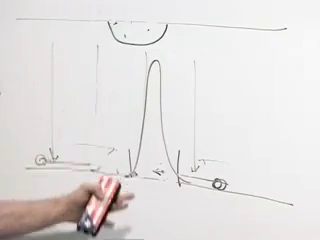
\includegraphics[width=0.82\textwidth]{lecture_05_figure_01.png}
\caption{第五维的地板与天花板图像。碰撞后，中央带有视界的能量块沿地板扩散。}
\lectureframe{00:04:22}
\end{figure}

视界不会永远存在。霍金辐射会带走能量，而在四维描述中，这种辐射就是从碰撞中涌现出的普通强子簇射。用这种语言来说，探测器事件中的数千条径迹就是从对偶黑洞中蒸发出的粒子。

\subsection{额外维度是真实的吗？}

\begin{classroomqa}
\audiencequestion{第五维是一个空间维度吗？地板与天花板之间画出的那条线是否真的沿该方向延伸？}
\lecturerresponse{是的。它是类空的，而在那个五维几何中画出的曲面就是一个视界。至于人们是把额外方向称为``真实的''，还是把它视为一种等价的数学描述，则是一个更深层的问题。}
\end{classroomqa}

有用的陈述并不是引力取代了量子色动力学。相反，两种语言可以描述同一物理。在四维语言中，存在一个由夸克和胶子组成的炽热火球，没有普通的引力场。在五维语言中，则存在引力和一个视界。如果这种对应关系是正确的，那么诚实的QCD计算和对偶引力计算在两者都能进行的地方必须一致。

\begin{classroomqa}
\audiencequestion{QCD既没有引力也没有视界。黑洞图像是在添加新物理，还是仅仅重新描述了火球？}
\lecturerresponse{在四维中，它是夸克和胶子的等离子体；在五维化身中，它有一个带视界的引力描述。优势在于计算。强耦合QCD极其困难，而某些视界性质---尤其是黏滞性---则相对容易计算。}
\end{classroomqa}

``真实维度''与``数学类比''之间的区分不必在描述变得有用之前就得到解决。当一个结构与其他变量结合成一组更简单、更连贯的定律时，它就获得了物理解释。尽管如此，人们不应夸大这一点：规范/引力对偶性对所观测到的夸克--胶子等离子体的应用，是强耦合动力学的模型，而不是证明现实世界中的QCD具有已知的精确引力对偶。\editorialnote{这一限定明确了QCD应用的现代地位；它并不改变此处所发展的五维机制。}

\section{为什么对撞机使束流对撞}

现在这些问题变得实际了。为什么要使用两束运动的束流，而不是一束束流加一个静止靶？为什么环形加速器如此之大？为什么电子和质子的处理方式不同？所有这些问题都是关于相对论能量的问题。

\begin{classroomqa}
\audiencequestion{为什么要让两束束流对撞，而不是将一束高能束流射向静止靶？}
\lecturerresponse{产生新粒子的是质心系中可用的能量。两束相等且方向相反的相对论束流没有净动量，因此它们的能量基本上全部可用于碰撞。固定靶则迫使大部分入射能量保留为质心的运动。}
\end{classroomqa}

对于两个具有大小为\(p\)的相反动量的超相对论粒子，在\(c=1\)单位下的讲义级估计为
\begin{equation}
E_{\mathrm{cm}}^{\mathrm{collider}}\simeq 2p.
\end{equation}
相应的固定靶估计仅按束流动量的平方根增长，
\begin{equation}
E_{\mathrm{cm}}^{\mathrm{fixed}}\sim \sqrt{mp}.
\end{equation}
关键在于这种标度关系，而不是被省略的数值因子：将束流能量加倍会使对撞机能量加倍，但只会使固定靶质心能量增加一个平方根。

不变量计算使比较变得精确。如果\(P_1\)和\(P_2\)是入射四维动量，那么
\begin{equation}
s=(P_1+P_2)^2,
\qquad E_{\mathrm{cm}}=\sqrt{s}.
\end{equation}
对于能量为\(E\)的等量反向传播束流，空间动量相互抵消，且\(\sqrt{s}=2E\)。对于能量为\(E\gg m\)的抛射粒子撞击静止的等质量靶，
\begin{equation}
s=2m^2+2mE,
\qquad
\sqrt{s}\simeq \sqrt{2mE}
\qquad (c=1).
\end{equation}
这一简短的不变量推导提供了口头估计中被压低的因子。\editorialnote{引入该推导是为了使讲义的标度论证可复现。}

\begin{classroomqa}
\audiencequestion{环形加速器必须如此之大，是否有根本原因？同一束流能否只是更多次地通过一台更小的机器循环？}
\lecturerresponse{场和材料施加了限制。粒子每米获得的能量增量是有限的，因此更高能量的机器需要更长的有效加速长度。紧凑的圆环还要求更大的横向加速度，而加速电荷会辐射。如果环太小，束流辐射能量的速度就会与机器供给能量的速度一样快。}
\end{classroomqa}

偏转关系近似为
\begin{equation}
p=qBR,
\end{equation}
因此对于固定的磁场\(B\)，更大的动量\(p\)需要更大的半径\(R\)。射频腔完成提高束流能量的功；磁铁使束流偏转并聚焦。广泛的教训仍然是黑板上给出的那一条：场强和辐射损失阻止我们将任意高能的加速器压缩成一个小环。

圆周运动即使在速率恒定时也有加速度，因为速度方向在改变。加速电荷会发射同步辐射。直线加速器避免了连续的偏转损失，尽管短的加速推动本身并非字面意义上的无辐射。环形机器接受偏转代价，以换取在每一圈上重复使用同一套装置。

\begin{classroomqa}
\audiencequestion{为什么电子与SLAC的直线机器相关联，而环形高能对撞机使用质子或其他强子？}
\lecturerresponse{电子要轻得多。在给定的高能量下，它们的洛伦兹因子大得多，而圆周加速使它们辐射得强烈得多。较重的质子可以反复循环，在每一圈上获得能量，直到同步辐射损失变得不可承受。}
\end{classroomqa}

对于固定的能量和环半径，辐射功率随粒子质量极其陡峭地变化，
\begin{equation}
P_{\mathrm{sync}}\propto \frac{E^4}{m^4R^2}.
\end{equation}
这就是为什么电子--质子之别远比``较轻的粒子运动得更快''这一说法所暗示的要鲜明得多：两束束流都可以已经极其接近\(c\)，但它们的洛伦兹因子和辐射损失却非常不同。\editorialnote{弯曲关系和同步辐射标度律使讲座中定性的加速器论证变得精确；这些并未在黑板上推导出来。}

\begin{classroomqa}
\audiencequestion{为什么不也把强子放在直线中加速呢？}
\lecturerresponse{可以。困难在于长度。在环中，同一粒子会多次经过加速结构；一台等效的直线强子机器则必须极其长。有用的折中方案是一个大环，大到质子辐射仍然可以容忍。}
\end{classroomqa}

这些加速器问题恰恰暴露出牛顿规则为何不够用。我们现在回到狭义相对论，并建立使这类比较系统化的语言。

\section{车库与加长轿车}

考虑一个约十二英尺长的车库和一辆约二十英尺长的加长轿车。司机不断加速，直到加长轿车发生洛伦兹收缩，希望它能装得下。在车库参考系中，运动中的加长轿车更短，所以看起来是可能的。然而在加长轿车参考系中，运动中的车库更短，所以看起来是不可能的。整辆加长轿车能同时位于车库内吗？

把两扇门都打开，这样就不会因撞到墙而分散我们的注意力。说加长轿车在里面，意味着它的前端和后端\emph{同时}都在里面。最后这个词包含了整个谜题。

画一个时空图，\(t\)竖直，\(x\)水平。在\(c=1\)单位下，光线构成\(45^\circ\)光锥。车库静止，所以它两扇门的世界线是竖直的。加长轿车的前端和后端描出两条平行的倾斜世界线。运动参考系的\(t'\)轴朝光锥方向倾斜，其同时性直线平行于倾斜的\(x'\)轴。

\begin{figure}[H]
\centering
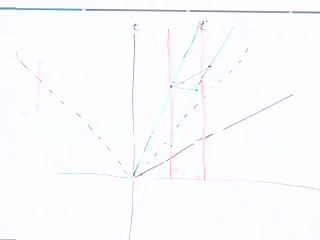
\includegraphics[width=0.82\textwidth]{lecture_05_figure_02.png}
\caption{完整的车库--加长轿车时空图。竖直线界定车库；斜线描出加长轿车的两端。水平切片和倾斜切片表示两个参考系不同的同时性切片。}
\lectureframe{00:31:05}
\end{figure}

在车库参考系中，一条水平线可以在两条车库世界线之间穿过两条加长轿车世界线。在那个车库时刻，后端已经进入，而前端尚未离开。收缩后的加长轿车完全在里面。

在加长轿车参考系中，相关的同时事件位于一条倾斜线上。过后端进入这一事件画这样一条线。它与前端世界线相交时，前端已经越过了远端那扇门。按照它自己的同时性，加长轿车从未完全在里面。两种说法都成立，因为它们比较的是不同的两对事件。

\begin{classroomqa}
\audiencequestion{两条绿色世界线以及它们之间的水平线段是否构成一个平行四边形？那条黑色线段是车辆的长度吗？}
\lecturerresponse{水平线段是洛伦兹收缩后的长度，因为它的端点在车库参考系中同时。固有长度则由在加长轿车参考系中同时的端点得到，位于平行于\(x'\)的直线上。这两种测量使用穿过同一对世界线的不同切片。}
\end{classroomqa}

如果\(L_0\)是固有长度，那么车库参考系中的水平切片长度为\begin{equation}
L=\frac{L_0}{\gamma},
\qquad
\gamma=\frac{1}{\sqrt{1-v^2/c^2}}.
\end{equation}
仅凭公式并不能解决这个悖论。图可以，因为它显示了比较的是哪些事件。每当一个相对论谜题似乎产生两个不相容的答案时，都要寻找对``同时''的未明言使用。

\section{四个坐标与两个指标位置}

要从谜题走向运动定律，我们需要一种能记住几何的记号。把坐标打包为
\begin{equation}
(X^1,X^2,X^3,X^0)=(x,y,z,t),
\qquad X^\mu=(x,y,z,t),
\end{equation}
其中\(\mu\)取遍\(1,2,3,0\)。这种排序把时间放在页面最后，尽管它的指标是\(0\)，与黑板上使用的约定一致。

\begin{classroomqa}
\audiencequestion{我们是在设定\(c=1\)吗？如果恢复普通单位，时间坐标是否应为\(ct\)？}
\lecturerresponse{是的。我们在展开几何时设定\(c=1\)，并在量纲或非相对论极限重要时把\(c\)的因子放回去。采用常规长度单位时，时间坐标是\(ct\)。}
\end{classroomqa}

同一个矢量也可以用下指标写出。按照这里采用的符号约定，
\begin{equation}
X_\mu=(-x,-y,-z,t).
\end{equation}
因此，降低一个指标会反转三个空间分量的符号，而时间分量保持不变。例如，
\begin{equation}
X^\mu=(3,2,4,10)
\quad\Longrightarrow\quad
X_\mu=(-3,-2,-4,10).
\end{equation}
这并不是两个时空点；它们是同一个几何对象的两种分量形式。

\begin{classroomqa}
\audiencequestion{哪些分量是协变的，哪些是逆变的，这些标记应该是上标还是下标？}
\lecturerresponse{上指标分量是逆变的；下指标分量是协变的。来自课堂的一个有用记忆法是``co 是低，contra 是高。''物理学家常常直接说“楼上”和“楼下”。}
\end{classroomqa}

这种记号在不变缩并中体现了其价值
\begin{equation}
X_\mu X^\mu=t^2-x^2-y^2-z^2.
\label{eq:l5-interval}
\end{equation}
用微分形式表示，这就是
\begin{equation}
d\tau^2=dt^2-dx^2-dy^2-dz^2
\qquad (c=1).
\label{eq:l5-proper-time}
\end{equation}
对于类时运动，\(d\tau\) 是沿世界线运动的时钟所记录的时间。

只要同一个指标在上方出现一次、在下方出现一次，就理解为对它求和。爱因斯坦约定把
\begin{equation}
\sum_{\mu}X_\mu X^\mu
\end{equation}
变成式~\eqref{eq:l5-interval}中更短的表达式。这不仅仅是排版上的节省。它防止闵可夫斯基几何中交替出现的符号在每一个方程中都被手工重写。

\begin{classroomqa}
\audiencequestion{\(\tau\) 是固有时（proper time）的标准符号吗？}
\lecturerresponse{是的。符号 \(s\) 有时也会被使用，但 \(\tau\) 是固有时的标准选择。}
\end{classroomqa}

\section{作为简单对称性的旋转}

洛伦兹助推混合空间和时间。在研究那个矩阵之前，先考虑更熟悉的操作：旋转空间坐标轴。如果相对运动指向任意方向，我们可以旋转坐标轴，直到该方向成为新的 \(x\) 轴，然后施加已知的助推。因此，旋转是这一构造的一部分，而不是装饰性的绕路。

对于绕 \(z\) 轴旋转角度 \(\theta\)，
\begin{align}
x'&=x\cos\theta+y\sin\theta,\nonumber\\
y'&=-x\sin\theta+y\cos\theta,\label{eq:l5-rotation}\\
z'&=z.\nonumber
\end{align}
在 \(\theta=0\) 时，这些方程给出 \(x'=x\) 和 \(y'=y\)；在 \(\theta=\pi/2\) 时，它们以预期的符号交换坐标轴。

该变换保持欧几里得距离不变。记
\(c_\theta=\cos\theta\) 和 \(s_\theta=\sin\theta\)，
\begin{align}
x'^2+y'^2
&=(xc_\theta+ys_\theta)^2+(-xs_\theta+yc_\theta)^2\nonumber\\
&=x^2(c_\theta^2+s_\theta^2)
  +y^2(s_\theta^2+c_\theta^2)\nonumber\\
&\quad+2xyc_\theta s_\theta-2xyc_\theta s_\theta\nonumber\\
&=x^2+y^2.
\end{align}
交叉项相消，且 \(c_\theta^2+s_\theta^2=1\)。由于 \(z'=z\)，整个长度 \(x^2+y^2+z^2\) 不变。

同样的方程可以写成一个矩阵方程：
\begin{equation}
\begin{pmatrix}x'\\y'\\z'\end{pmatrix}
=
\underbrace{\begin{pmatrix}
\cos\theta&\sin\theta&0\\
-\sin\theta&\cos\theta&0\\
0&0&1
\end{pmatrix}}_{M}
\begin{pmatrix}x\\y\\z\end{pmatrix}.
\label{eq:l5-rotation-matrix}
\end{equation}
用指标记号表示，
\begin{equation}
x'^i=M^i{}_{j}x^j,
\qquad i,j=1,2,3.
\end{equation}

\begin{figure}[H]
\centering
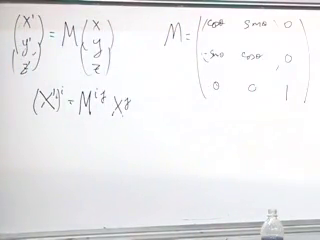
\includegraphics[width=0.82\textwidth]{lecture_05_figure_03.png}
\caption{空间旋转既写成矩阵方程，也写成指标记号。}
\lectureframe{01:00:40}
\end{figure}

\section{洛伦兹矩阵与速度合成}

对于沿 \(x\) 方向的运动，在 \(c=1\) 单位下的洛伦兹变换为
\begin{align}
x'&=\gamma_v(x-vt), & y'&=y,\nonumber\\
z'&=z, & t'&=\gamma_v(t-vx),
\end{align}
其中
\begin{equation}
\gamma_v=\frac{1}{\sqrt{1-v^2}}.
\end{equation}
采用分量顺序 \((x,y,z,t)\)，这变为
\begin{equation}
\begin{pmatrix}x'\\y'\\z'\\t'\end{pmatrix}
=
\begin{pmatrix}
\gamma_v&0&0&-\gamma_vv\\
0&1&0&0\\
0&0&1&0\\
-\gamma_vv&0&0&\gamma_v
\end{pmatrix}
\begin{pmatrix}x\\y\\z\\t\end{pmatrix}.
\label{eq:l5-lorentz-matrix}
\end{equation}

\begin{figure}[H]
\centering
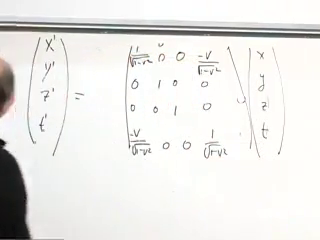
\includegraphics[width=0.82\textwidth]{lecture_05_figure_04.png}
\caption{\(4\times4\) 洛伦兹矩阵。只有 \(x\) 和 \(t\) 分量混合；\(y\) 和 \(z\) 保持不变。}
\lectureframe{01:04:40}
\end{figure}

矩阵乘法现在回答一个物理问题。假设一个观察者相对于我们以速度 \(v\) 运动，而第三个观察者相对于该观察者以速度 \(u\) 运动，全都沿同一轴。牛顿运动学会给出 \(w=u+v\)，这会使两个 \(3c/4\) 的速度合成为 \(3c/2\)。相对论必须给出不同的规则。

助推的有效部分是 \(2\times2\) 矩阵
\begin{equation}
B(v)=\gamma_v
\begin{pmatrix}1&-v\\-v&1\end{pmatrix}.
\end{equation}
将两个助推复合得到
\begin{align}
B(u)B(v)
&=\gamma_u\gamma_v
\begin{pmatrix}1&-u\\-u&1\end{pmatrix}
\begin{pmatrix}1&-v\\-v&1\end{pmatrix}\nonumber\\
&=\gamma_u\gamma_v
\begin{pmatrix}
1+uv&-(u+v)\\
-(u+v)&1+uv
\end{pmatrix}.
\label{eq:l5-composed-boost}
\end{align}
非对角元与对角元之比确定了合成助推的速度：
\begin{equation}
w=\frac{u+v}{1+uv}
\qquad(c=1).
\end{equation}
恢复量纲后，
\begin{equation}
w=\frac{u+v}{1+uv/c^2}.
\label{eq:l5-velocity-addition}
\end{equation}

\begin{figure}[H]
\centering
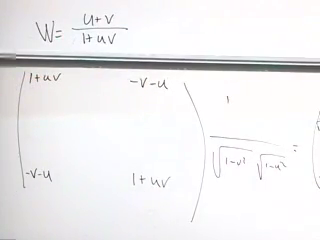
\includegraphics[width=0.82\textwidth]{lecture_05_figure_05.png}
\caption{复合助推矩阵以及自然单位下的速度 \(w=(u+v)/(1+uv)\)。}
\lectureframe{01:15:35}
\end{figure}

如果 \(u\) 和 \(v\) 都接近 \(c\)，则分子趋近 \(2c\)，而分母趋近 \(2\)，所以 \(w\) 趋近 \(c\)，而不是 \(2c\)。更一般地，式~\eqref{eq:l5-velocity-addition}把亚光速输入映射为亚光速结果。矩阵乘法自动编码了速度极限。

\section{四维矢量与普通速度的失效}

四维矢量是任何其四个分量在旋转和洛伦兹助推下与时空坐标以相同方式变换的对象。如果 \(V^\mu\) 是四维矢量，那么按照我们的符号约定
\begin{equation}
V_\mu=(-V^1,-V^2,-V^3,V^0),
\end{equation}
其不变模长为
\begin{equation}
V_\mu V^\mu=(V^0)^2-(V^1)^2-(V^2)^2-(V^3)^2.
\end{equation}
对于两个四维矢量 \(V^\mu\) 和 \(W^\mu\)，缩并
\begin{equation}
W_\mu V^\mu
=W^0V^0-W^1V^1-W^2V^2-W^3V^3
\end{equation}
同样不变。分量在不同参考系之间改变；缩并则不变。

普通速度只有三个分量，
\begin{equation}
\mathbf v=\left(\frac{dx}{dt},\frac{dy}{dt},\frac{dz}{dt}\right).
\end{equation}
附加 \(dt/dt=1\) 并不能使它成为有用的四维矢量。第四个分量
将是平凡的，而且所得对象在洛伦兹变换下不会线性变换。坐标时 \(t\) 从一个参考系到
另一个参考系会改变，因此对 \(t\) 求导会破坏所期望的变换律。

固有时提供了解决办法。沿一条世界线定义
\begin{equation}
u^\mu=\frac{dX^\mu}{d\tau}.
\label{eq:l5-four-velocity}
\end{equation}
微分 \(dX^\mu\) 是四维矢量，而 \(d\tau\) 是不变量，所以
二者之比是四维矢量。形容词 ``固有'' 指的是
分母中的时钟。

链式法则将这个对象与普通速度联系起来：
\begin{equation}
\frac{dx}{d\tau}=\frac{dx}{dt}\frac{dt}{d\tau},
\end{equation}
对 \(y\) 和 \(z\) 也类似。由
式~\eqref{eq:l5-proper-time}，
\begin{align}
\left(\frac{d\tau}{dt}\right)^2
&=1-\left(\frac{dx}{dt}\right)^2
    -\left(\frac{dy}{dt}\right)^2
    -\left(\frac{dz}{dt}\right)^2\nonumber\\
&=1-v^2
\qquad(c=1),
\end{align}
因此
\begin{equation}
\frac{dt}{d\tau}=\gamma_v=\frac{1}{\sqrt{1-v^2}}.
\end{equation}
四个分量为
\begin{equation}
u^i=\gamma_v v^i,
\qquad
u^0=\gamma_v
\qquad(c=1).
\label{eq:l5-four-velocity-components}
\end{equation}
在低速下，\(u^i\simeq v^i\) 且 \(u^0\simeq1\)。接近光速时，
\(\gamma_v\) 无界增长，固有速度与
普通速度差别很大。

\begin{figure}[H]
\centering
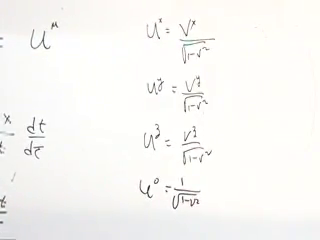
\includegraphics[width=0.82\textwidth]{lecture_05_figure_06.png}
\caption{用普通速度和洛伦兹因子表示的固有速度的四个分量。}
\lectureframe{01:34:40}
\end{figure}

恢复常规单位并使用 \(X^0=ct\)，得到标准形式
\begin{equation}
U^\mu=(\gamma_v\mathbf v,\gamma_v c)
\end{equation}
这里采用空间分量在前的排序。其不变模长为
\begin{equation}
U_\mu U^\mu=c^2.
\end{equation}
因此每个有质量粒子都具有相同不变
大小的四维速度，尽管其空间速度依赖于参考系。

\section{世界线的切矢量}

对于式~\eqref{eq:l5-four-velocity}，有一个熟悉的欧几里得模型。
沿普通三维空间中的一条曲线，
\begin{equation}
ds^2=dx^2+dy^2+dz^2.
\end{equation}
微分位移 \((dx,dy,dz)\) 沿曲线方向，但
不是单位矢量。除以弧长得到
\begin{equation}
\mathbf T=
\left(\frac{dx}{ds},\frac{dy}{ds},\frac{dz}{ds}\right),
\qquad
\mathbf T\cdot\mathbf T=1.
\end{equation}
相对论构造是同样的想法，只是用固有时代替
欧几里得弧长。矢量 \(u^\mu=dX^\mu/d\tau\) 与
世界线相切。

\begin{figure}[H]
\centering
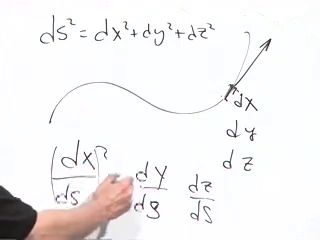
\includegraphics[width=0.82\textwidth]{lecture_05_figure_07.png}
\caption{欧几里得切矢量构造：将微分
位移除以弧长元 \(ds\)。固有时沿类时世界线扮演类似
角色。}
\lectureframe{01:39:30}
\end{figure}

\begin{classroomqa}
\audiencequestion{如果 \(c=1\)，那么固有时和固有距离相同吗？}
\lecturerresponse{令 \(c=1\) 使时间和距离具有相同单位；这
并不会消除时空几何的负号。在欧几里得类比中，
\(s\) 是沿空间曲线测量的普通距离。沿类时
世界线，\(\tau\) 是由时钟测量的流逝时间。这些构造
类似，但几何不同。}
\end{classroomqa}

再求一次导数定义固有加速度，
\begin{equation}
a^\mu=\frac{du^\mu}{d\tau}.
\end{equation}
当牛顿
第二定律被相对论化时，必须用这个量代替 \(d^2\mathbf x/dt^2\)。由于 \(u_\mu u^\mu\) 是常数，
\begin{equation}
\frac{d}{d\tau}(u_\mu u^\mu)=2u_\mu a^\mu=0,
\end{equation}
所以四维加速度与四维速度闵可夫斯基正交。\editorialnote{这种
正交性立即由不变模长得出，并作为该定义的下一项数学推论列入。}

\section{四维动量和能量}

动量是我们的最后一个例子，因为它在碰撞和衰变中守恒。
粒子具有固定的内禀质量 \(m\)，通常称为其静止质量。它
不随速度变化。相对论动量就是这个固定质量乘以
四维速度：
\begin{equation}
p^\mu=mu^\mu.
\label{eq:l5-four-momentum}
\end{equation}
在 \(c=1\) 单位下，
\begin{equation}
p^i=\gamma_v m v^i,
\qquad
p^0=\gamma_v m.
\end{equation}
在低速下 \(\gamma_v\simeq1\)，所以空间分量约化为
牛顿动量 \(m\mathbf v\)。在高速下它们比 \(m\mathbf v\) 增长得更快。

时间分量是能量。采用常规单位并使用 \(X^0=ct\)，
\begin{equation}
P^\mu=(\mathbf p,E/c)
=(\gamma_v m\mathbf v,\gamma_v mc),
\end{equation}
因此
\begin{equation}
E=\gamma_v mc^2
=mc^2\left(1-\frac{v^2}{c^2}\right)^{-1/2}.
\label{eq:l5-relativistic-energy}
\end{equation}

为了恢复普通力学，令
\(\epsilon=v^2/c^2\ll1\)。二项式展开给出
\begin{equation}
(1-\epsilon)^p=1-p\epsilon+O(\epsilon^2).
\end{equation}
取 \(p=-1/2\)，
\begin{align}
E
&=mc^2\left(1-\frac{v^2}{c^2}\right)^{-1/2}\nonumber\\
&=mc^2\left[1+\frac12\frac{v^2}{c^2}
  +O\!\left(\frac{v^4}{c^4}\right)\right]\nonumber\\
&=mc^2+\frac12mv^2+O\!\left(\frac{mv^4}{c^2}\right).
\label{eq:l5-energy-expansion}
\end{align}

\begin{figure}[H]
\centering
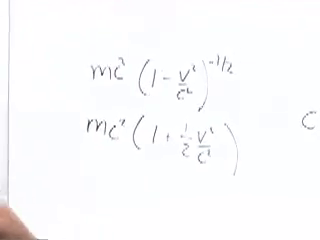
\includegraphics[width=0.82\textwidth]{lecture_05_figure_08.png}
\caption{相对论能量的低速展开，揭示出静止
能量和牛顿动能。}
\lectureframe{01:51:30}
\end{figure}

第一项 \(mc^2\) 即使在静止时也存在。在一个具有
固定粒子集合且质量不变的牛顿问题中，该项在
运动前后加上相同的常数，所以只有 \(\tfrac12mv^2\) 影响
熟悉的记账。相对论揭示出，被丢弃的常数一直都是
物理能量。

因此能量和动量并非互不相关的守恒定律。它们是
一个守恒矢量的四个分量。洛伦兹助推将它们混合：一个
观察者称为能量的东西部分地贡献给另一个观察者的动量，
反之亦然。尽管如此，对于孤立系统，总四维动量
在每个惯性参考系中于每次碰撞或衰变前后都相同。

这是相对论力学的门槛。接下来的任务是用力固有加速度来表示力，并理解相对论性波动方程，尤其是支配电磁学和光的方程。
\chapter{不变定律、四维矢量与场张量}

我们将从一条自然界本可以遵守、却并未遵守的定律开始。它的失效将告诉我们，一条物理定律应当如何书写。同样的检验首先把坐标分量引向普通矢量，继而把普通矢量引向四维矢量，最终把四维矢量引向张量。到末尾时，电场与磁场将不再是彼此分离的对象：它们将共同占据一个反对称张量的六个独立位置。

除非另有说明，我们采用\(c=1\)的单位制，将时空分量排序为\((1,2,3,0)=(x,y,z,t)\)，并使用度规号差\((-,-,-,+)\)。

\section{一条对称性错误的可能定律}

在空间中永久固定一条\(x\)轴和一条\(y\)轴。现在规定：只要两个粒子的\(x\)坐标相同，它们就发生相互作用。这种相互作用可能使它们的运动反向，也可能把它们送往新的方向；其具体动力学并不重要。所提出的触发条件仅仅是
\begin{equation}
  x_1-x_2=0,
\end{equation}
其中下标标记的是粒子，而不是坐标分量。这条规则在数学上并无矛盾。问题在于，它为何在物理上不可信。

\begin{classroomqa}
\audiencequestion{这条规则违反空间均匀性吗？}
\lecturerresponse{不违反。平移原点会使两个坐标改变相同的量，因而\(x_1-x_2\)保持不变。这条规则并未指定任何优先位置。它的缺陷在于各向同性：它挑出了一个优先方向。}
\end{classroomqa}

将坐标轴旋转\(90^\circ\)。原来的\(x\)方向现在称为\(y\)，因此同样的物理事件将被描述为\(y\)坐标相等。在一般角度下，该条件将涉及\(x\)与\(y\)的线性组合。于是，这条定律的形式取决于黑板是如何摆放的。它具有平移不变性，却不具有旋转不变性。

我们通常让物理定律在正交坐标中取最简形式。人们可以使用更一般的坐标，但那样度规和公式就会变得不那么简单。在正交笛卡儿坐标系的类别之内，任何取向都不应享有特权。

修正立即可得。在二维中要求两个坐标都相同；在三维中要求三个坐标都相同：
\begin{equation}
  x_1=x_2,
  \qquad y_1=y_2,
  \qquad z_1=z_2.
\end{equation}
于是，粒子只有在到达同一点时才能相互作用，即使它们沿不同直线趋近该点。

\begin{classroomqa}
\audiencequestion{\(z\)坐标和时间也必须相同吗？}
\lecturerresponse{在三维空间中，\(z\)坐标也必须相同。时间暂时被略去；一旦空间论证完成，它就会被恢复。}
\end{classroomqa}

设\(\boldsymbol r_a\)为粒子\(a\)的位置。三个分量条件变成一个矢量方程，
\begin{equation}
  \boldsymbol r_1-\boldsymbol r_2=\boldsymbol 0.
\end{equation}
一个分量可以在某个旋转后的坐标系中为零，而在另一个坐标系中不为零。整个矢量则不同：如果在一个坐标系中每个分量都为零，那么在每个旋转后的坐标系中每个分量也都为零。同样，如果两个矢量在一个坐标系中相等，那么在对二者都作变换之后，它们仍然相等。

\begin{figure}[H]
\centering
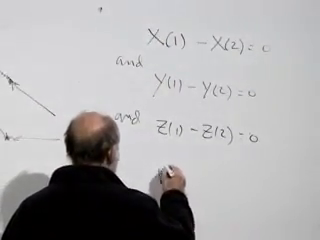
\includegraphics[width=0.78\textwidth]{lecture_06_figure_01.png}
\caption{使碰撞意味着空间重合、而非沿某一优先轴重合的三个坐标等式。}
\lectureframe{00:09:00}
\end{figure}

这就是矢量方程之所以有用的原因。它们的分量会改变，但对象会协调地变换。为完整对象写出的定律，在坐标旋转时能够保持其形式。

\section{时空中的重合}

现在把竖直的空间轴换成时间。一条牛顿式规则可能会说：两次运动变化只有在时间相等时才发生。在牛顿力学中，同时性为所有惯性观察者所共有，因此这样的规则是可能的。在狭义相对论中，它却挑出了一个优先参考系。在一个参考系中同时的事件，在另一个参考系中未必同时。

只要求空间坐标相等也好不到哪里去。一个时空位移可以具有为零的空间分量和一个非零的时间分量，
\begin{equation}
  \Delta X^\mu=(0,0,0,\Delta t),
\end{equation}
而一个助推会把\(\Delta t\)与某个空间分量混合起来。不变性的局域陈述是：两次运动变化发生在同一事件处。因此，一次简单的碰撞要求
\begin{equation}
  X_1^\mu=X_2^\mu,
  \qquad\text{or}\qquad
  X_1^\mu-X_2^\mu=0.
\end{equation}
四个坐标全都相同：粒子在同一时间占据同一地点。

碰撞这个例子给出了书写物理学的一条一般规则。我们可以把所有东西放到一边，令一个完整的四维矢量等于零，或者令一个完整的四维矢量等于另一个。把四维矢量中互不相关的部分彼此等同，本身并不能给出洛伦兹不变的陈述。

\section{助推、旋转与矩阵记法}

四维矢量是这样一种对象：它的变换方式与时空位移的变换方式相同。
为了使这个定义有用，首先回顾坐标本身的变换。对于沿\(x\)方向、速度为\(v\)的助推，
\begin{align}
  x'&=\gamma(x-vt), & y'&=y, & z'&=z,
  & t'&=\gamma(t-vx),                                      \label{eq:l6-boost}
\end{align}
其中
\begin{equation}
  \gamma(v)=\frac{1}{\sqrt{1-v^2}}.
\end{equation}

\begin{classroomqa}
\audiencequestion{在这些公式中，光速是否已被设为1？}
\lecturerresponse{是的。恢复单位后，取\(X^0=ct\)，将\(1-v^2\)替换为\(1-v^2/c^2\)，并在混合的空间--时间项中恢复相应的\(c\)因子。}
\end{classroomqa}

绕\(z\)轴的旋转混合\(x\)和\(y\)，而\(z\)和\(t\)保持不变：
\begin{equation}
\begin{pmatrix}
  x'\\ y'\\ z'\\ t'
\end{pmatrix}
=
\begin{pmatrix}
  \cos\theta & \sin\theta & 0 & 0\\
  -\sin\theta & \cos\theta & 0 & 0\\
  0 & 0 & 1 & 0\\
  0 & 0 & 0 & 1
\end{pmatrix}
\begin{pmatrix}
  x\\ y\\ z\\ t
\end{pmatrix}.
\end{equation}
其中的零值得展示出来：它们明确显示了哪些分量不进入某个给定的变换后坐标。按同样的排列顺序，式~\eqref{eq:l6-boost}中的助推为
\begin{equation}
\begin{pmatrix}
  x'\\ y'\\ z'\\ t'
\end{pmatrix}
=
\begin{pmatrix}
  \gamma & 0 & 0 & -\gamma v\\
  0 & 1 & 0 & 0\\
  0 & 0 & 1 & 0\\
  -\gamma v & 0 & 0 & \gamma
\end{pmatrix}
\begin{pmatrix}
  x\\ y\\ z\\ t
\end{pmatrix}.
\end{equation}

旋转和助推可以通过矩阵乘法复合。要沿与原始\(x\)轴不对齐的方向进行助推，可以先将该方向旋转到\(x\)轴，施加助推，再按需旋转回去。这些初等矩阵的乘积生成更一般的洛伦兹变换。

\begin{classroomqa}
\audiencequestion{先旋转再助推，还是先助推再旋转，这有区别吗？}
\lecturerresponse{有。第一次操作之后，第二次操作所作用的轴已经改变了。两个矩阵乘积不必相等，因此操作的顺序是有关系的。}
\end{classroomqa}

所有这些线性变换可以一次性写成
\begin{equation}
  X'^{\mu}=\Lambda^{\mu}{}_{\nu}X^{\nu}.                  \label{eq:l6-vector-transform}
\end{equation}
重复指标\(\nu\)对\(1,2,3,0\)求和。这不过是矩阵乘法中通常的逐行逐列求和，用指标记号表达出来而已。

\begin{figure}[H]
\centering
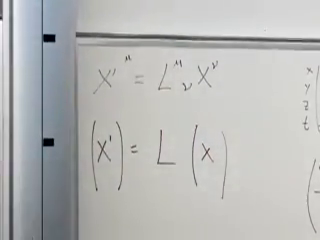
\includegraphics[width=0.78\textwidth]{lecture_06_figure_02.png}
\caption{上述带指标的洛伦兹变换，位于其列矢量形式的开头。}
\lectureframe{00:31:55}
\end{figure}

式~\eqref{eq:l6-vector-transform}也是一般逆变四维矢量的定义。如果\(A^\mu\)是这样一个矢量，那么
\begin{equation}
  A'^{\mu}=\Lambda^{\mu}{}_{\nu}A^{\nu}.
\end{equation}
它的四个分量不必表示位置。使这个对象成为四维矢量的是它的变换规律。

\section{标量、度规与不变量乘积}

在使用更多四维矢量之前，退回到更简单的标量概念是有帮助的。在空间旋转下，指定点处的温度是一个标量，两个指定点之间的距离也是一个标量。它们各自是一个数，与坐标轴的取向无关。人们甚至可以故意提出一个愚蠢的数值断言：以厘米测量的距离等于以华氏度测量的室温。这个断言没有物理深度，但由于两边都是旋转标量，其真假并不取决于坐标轴如何转动。

矢量的分量不是标量。因此我们需要一种系统的方法将它们组合成标量。将一般逆变四维矢量写成
\begin{equation}
  A^\mu=(A^1,A^2,A^3,A^0).
\end{equation}
协变分量用下指标描述同一个几何对象。在我们的号差下，它们通过闵可夫斯基度规得到，
\begin{equation}
  A_\mu=\eta_{\mu\nu}A^\nu,
  \qquad
  \eta_{\mu\nu}=
  \begin{pmatrix}
    -1&0&0&0\\
    0&-1&0&0\\
    0&0&-1&0\\
    0&0&0&1
  \end{pmatrix},                                          \label{eq:l6-metric}
\end{equation}
于是
\begin{equation}
  A_\mu=(-A^1,-A^2,-A^3,A^0).
\end{equation}

\begin{classroomqa}
\audiencequestion{黑板上的两个指标和符号不一致吗？}
\lecturerresponse{是的。所展示的列中的空间分量需要相应的负号，而指标下降方程右边的分量在乘以\(\eta_{\mu\nu}\)之前带有上指标。时间标签是\(0\)，不是\(4\)。}
\end{classroomqa}

\begin{figure}[H]
\centering
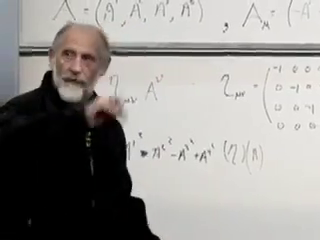
\includegraphics[width=0.8\textwidth]{lecture_06_figure_03.png}
\caption{逆变分量与协变分量、度规矩阵，以及不变量缩并的开头。}
\lectureframe{00:45:00}
\end{figure}

指标下降不是装饰。它把洛伦兹不变模长所需的符号打包在一起：
\begin{align}
  A_\mu A^\mu
  &=-(A^1)^2-(A^2)^2-(A^3)^2+(A^0)^2,                    \label{eq:l6-norm}\\
  X_\mu X^\mu
  &=t^2-x^2-y^2-z^2.
\end{align}
第二个表达式是从原点出发的不变时空间隔。因为\(A^\mu\)的变换方式与\(X^\mu\)相同，所以它的缩并具有同样的不变性。

这种记号还教给我们一条有用的记账规则。重复的求和指标一次出现在上方，一次出现在下方。例如，
\begin{equation}
  A_\mu A^\mu
  =\eta_{\mu\nu}A^\mu A^\nu.
\end{equation}
被求和指标（哑指标）的名称可以改变，而不改变该量。

\begin{classroomqa}
\audiencequestion{这些矢量中的一个是否应被视为行，另一个被视为列，它们的顺序有关系吗？}
\lecturerresponse{就当前的计算而言，把带指标的这些量视为分量，让度规来完成缩并；没有必要把讨论变成行与列的算符代数。这些都是普通数，所以它们的顺序没有关系。非对易算符需要更小心，但这不是这里的主题。}
\end{classroomqa}

同样的构造给出两个不同四维矢量之间的内积，
\begin{equation}
  A\mathbin{\cdot}B=A_\mu B^\mu=A^\mu B_\mu.
\end{equation}
无需写出显式的洛伦兹矩阵即可得到其不变性。由于
\(A+B\) 和 \(A-B\) 是四维矢量，它们的模平方都是
不变的：
\begin{align}
  (A+B)^2&=A^2+B^2+2A\mathbin{\cdot}B,\\
  (A-B)^2&=A^2+B^2-2A\mathbin{\cdot}B.
\end{align}
相减得到
\begin{equation}
  (A+B)^2-(A-B)^2=4A\mathbin{\cdot}B,                    \label{eq:l6-polarization}
\end{equation}
因此 \(A\mathbin{\cdot}B\) 也是不变的。因子四直接来自该展开。\editorialnote{黑板上的论证给出了这个
极化恒等式；写出该因子使口头讲述的相消变得明确无误。}

\begin{figure}[H]
\centering
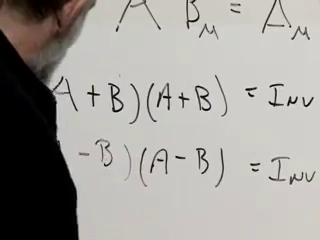
\includegraphics[width=0.8\textwidth]{lecture_06_figure_04.png}
\caption{用于分离不同四维矢量内积的两个不变平方。}
\lectureframe{00:52:20}
\end{figure}

不变量是物理定律的天然组成部分：与孤立的
分量不同，它在不同参考系中取相同的值。

\section{固有速度和四维动量}

考虑粒子世界线上的两个相邻事件。它们的间隔
是无穷小四维矢量
\begin{equation}
  dX^\mu=(dx,dy,dz,dt).
\end{equation}
对于类时世界线，固有时间定义为
\begin{equation}
  d\tau^2=dX_\mu dX^\mu
  =dt^2-dx^2-dy^2-dz^2.                                  \label{eq:l6-proper-time}
\end{equation}
固有四维速度为
\begin{equation}
  U^\mu=\frac{dX^\mu}{d\tau}.                            \label{eq:l6-four-velocity}
\end{equation}
它衡量的是时空位置相对于粒子自身固有时间的变化率，
而不是相对于所选参考系的坐标时间。

尽管 \(U^\mu\) 有四个分量，但只有三个是独立的。将
式~\eqref{eq:l6-proper-time}除以 \(d\tau^2\) 得到
\begin{equation}
  U_\mu U^\mu=1.
\end{equation}
因此四维速度是单位类时矢量。取指向未来的选择
确定了其时间分量的符号。

\begin{classroomqa}
\audiencequestion{在远小于 \(c\) 的速度下，四维速度是否约化为
普通速度？}
\lecturerresponse{它的三个空间分量趋近于普通速度，
而时间分量在 \(c=1\) 单位下趋近于一。该关系通过
应用链式法则并计算 \(dt/d\tau\) 得到。}
\end{classroomqa}

对每个空间分量，
\begin{equation}
  U^i=\frac{dx^i}{d\tau}
     =\frac{dx^i}{dt}\frac{dt}{d\tau}
     =v^i\frac{dt}{d\tau}.
\end{equation}
将式~\eqref{eq:l6-proper-time}除以 \(dt^2\)：
\begin{equation}
  \left(\frac{d\tau}{dt}\right)^2
  =1-v_x^2-v_y^2-v_z^2
  =1-\boldsymbol v^2.
\end{equation}
因此
\begin{equation}
  \frac{dt}{d\tau}=\frac{1}{\sqrt{1-\boldsymbol v^2}}
  =\gamma(\lvert\boldsymbol v\rvert),
\end{equation}
以及
\begin{equation}
  U^\mu=(\gamma v_x,\gamma v_y,\gamma v_z,\gamma).
                                                                  \label{eq:l6-u-components}
\end{equation}

\begin{figure}[H]
\centering
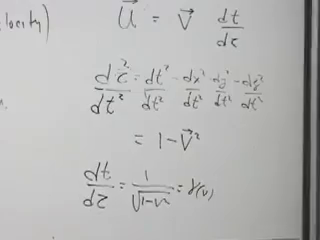
\includegraphics[width=0.8\textwidth]{lecture_06_figure_05.png}
\caption{产生 \(dt/d\tau=\gamma\) 并将固有速度与普通速度联系起来的
固有时间计算。}
\lectureframe{01:02:00}
\end{figure}

\begin{classroomqa}
\audiencequestion{\(dx^2/dt^2\) 是否表示二阶导数，并且
对矢量取平方是否应产生交叉项？}
\lecturerresponse{这里它表示 \((dx/dt)^2\)，即一阶导数的平方。此外，\(\boldsymbol v^2\) 表示欧几里得点积
\(v_x^2+v_y^2+v_z^2\)，而不是形式上的和
\(v_x+v_y+v_z\) 的平方；不存在交叉项。}
\end{classroomqa}

\begin{classroomqa}
\audiencequestion{\(\gamma(v)\) 中的 \(v\) 是两个坐标参考系的
相对速度，还是粒子的速度？}
\lecturerresponse{这里是粒子在所选参考系中的速度。
函数 \(\gamma(v)=1/\sqrt{1-v^2}\) 可以对任意速度求值：在
助推中它按参考系的相对速度求值；在四维速度中它
按粒子速度求值。}
\end{classroomqa}

对于 \(v\ll1\)，\(\gamma\simeq1\)，因此 \(U^\mu\) 的空间分量
趋近于 \(\boldsymbol v\)，而 \(U^0\) 趋近于一。当普通速度
趋近于光速时，\(\gamma\) 以及四维速度的所有非零分量
都无界增长。

\begin{classroomqa}
\audiencequestion{\(U^0\) 难道不应该具有速度的量纲，而不是
接近数字一吗？}
\lecturerresponse{当 \(c\) 被设为一后，量纲就消失了。在
\(X^0=ct\) 下，有
\(U^\mu=(\gamma\boldsymbol v,\gamma c)\)，因此时间分量趋近于
\(c\)，且 \(U_\mu U^\mu=c^2\)。}
\end{classroomqa}

对于静质量为 \(m\) 的粒子，四维动量定义为
\begin{equation}
  P^\mu=mU^\mu.
\end{equation}
在自然单位下，
\begin{equation}
  P^\mu=(\gamma m\boldsymbol v,\gamma m).
\end{equation}
前三个分量在低速下趋近于牛顿动量 \(m\boldsymbol v\)。恢复量纲后得到
\begin{equation}
  P^\mu=(\gamma m\boldsymbol v,E/c),
  \qquad E=\gamma mc^2,
\end{equation}
从而
\begin{equation}
  E=mc^2+\frac{1}{2}m\boldsymbol v^2+O(mv^4/c^2).
\end{equation}
时间分量是以 \(c=1\) 为单位的能量，或者当
四个分量都被赋予动量单位时，是能量除以 \(c\)。

\begin{classroomqa}
\audiencequestion{把普通 \(\boldsymbol v\) 附加第四个分量后，
它本身是四维矢量吗？}
\lecturerresponse{不是。普通三维速度不按
四维矢量变换。因子 \(\gamma\) 和固有时间的定义是
本质性的；四维矢量是 \(U^\mu\)，而不是 \(\boldsymbol v\)。}
\end{classroomqa}

\section{为什么电场和磁场必须混合}

我们现在暂时离开相对论，作一次所谓的短暂休假。从
前爱因斯坦运动方程出发，并追问在它
能在每个惯性系中成立之前必须如何被重新组织。普通加速度是普通速度的
时间导数。它的四维类似物自然是
\begin{equation}
  A^\mu=\frac{dU^\mu}{d\tau}.
\end{equation}
在低速下其空间分量趋近于普通加速度。完整的
相对论方程将推迟讨论；首先考察旧的力定律。

对于在电场和磁场中运动的电荷\(q\)，
\begin{equation}
  \boldsymbol F=m\boldsymbol a
  =q\left(\boldsymbol E+\boldsymbol v\times\boldsymbol B\right).
                                                                  \label{eq:l6-lorentz-force}
\end{equation}
电场项与粒子速度无关，而磁场项则不然。

\begin{figure}[H]
\centering
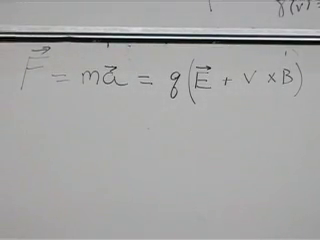
\includegraphics[width=0.8\textwidth]{lecture_06_figure_06.png}
\caption{促使人们将\(\boldsymbol E\)与\(\boldsymbol B\)结合起来的前相对论形式的洛伦兹力定律。}
\lectureframe{01:18:20}
\end{figure}

假设一位观测者看不到电场，但看到了磁场和一个运动电荷。该电荷感受到磁力。然而，在电荷的瞬时静止参考系中，\(\boldsymbol v=0\)，因此式~\eqref{eq:l6-lorentz-force}中的磁场项消失。物理世界线并不会仅仅因为坐标改变就变成惯性的；因此新参考系中的力必须包含电场的贡献。更仔细地说，非零的四维加速度不能通过改变惯性参考系而变换为零，尽管三维加速度及其分量确实会变换。\editorialnote{这一关于四维加速度的陈述是课堂论证的不变形式，并且避免了将普通的三维加速度本身视为参考系不变量。}

因此，电场和磁场必须相互变换。它们合起来有六个分量，所以它们既不是一个标量，也不是一个四维矢量。我们需要一个新的变换对象。

\section{张量：每个指标对应一次变换}

标量可以称为零阶张量；它没有指标。四维矢量是一阶张量；它有一个指标，可取四个值。最简单的二阶例子是乘积
\begin{equation}
  A^\mu B^\nu.
\end{equation}
每个指标有四个值，因此该对象有\(4^2=16\)个分量，可以显示为一个\(4\times4\)阵列。三个矢量的乘积，
\begin{equation}
  A^\mu B^\nu C^\sigma,
\end{equation}
有\(4^3=64\)个分量，是三阶张量。更高阶继续遵循这一模式。名称不如定义该对象的规则重要。

如果
\begin{equation}
  A'^{\mu}=\Lambda^\mu{}_{\nu}A^\nu,
  \qquad
  B'^{\sigma}=\Lambda^\sigma{}_{\tau}B^\tau,
\end{equation}
那么它们的乘积变换为
\begin{equation}
  A'^{\mu}B'^{\sigma}
  =\Lambda^\mu{}_{\nu}\Lambda^\sigma{}_{\tau}
   A^\nu B^\tau.
\end{equation}
这给出了逆变二阶张量的定义定律：
\begin{equation}
  T'^{\mu\sigma}
  =\Lambda^\mu{}_{\nu}\Lambda^\sigma{}_{\tau}T^{\nu\tau}.
                                                                  \label{eq:l6-tensor-transform}
\end{equation}
每个指标对应一个洛伦兹矩阵。重复的\(\nu\)和\(\tau\)被求和；开放的\(\mu\)和\(\sigma\)标记在带撇参考系中正在计算的哪个分量。

\begin{figure}[H]
\centering
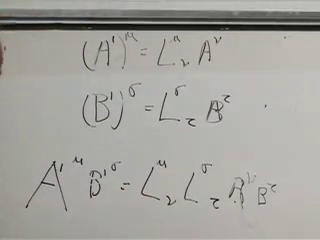
\includegraphics[width=0.82\textwidth]{lecture_06_figure_07.png}
\caption{两个矢量的变换以及由此得到的二阶张量的双矩阵变换定律。}
\lectureframe{01:27:15}
\end{figure}

张量不必是矢量的单一乘积。\(A^\mu B^\nu\)和\(A^\nu B^\mu\)都遵循张量变换定律，它们的和以及任何诸如
\begin{equation}
  A^\mu B^\nu+C^\mu D^\nu.
\end{equation}
这样的和也遵循。定义是变换定律，而不是某种特定的因式分解。三阶张量会获得第三个洛伦兹矩阵，依此类推。

\section{对称张量和反对称张量}

两类二阶张量将特别有用。对称张量满足
\begin{equation}
  T^{\mu\nu}=T^{\nu\mu},
\end{equation}
因此关于对角线反射的矩阵元相等。它的四个对角元和对角线一侧的六个矩阵元决定了其余部分，给出
\begin{equation}
  4+6=10
\end{equation}
个独立分量。

反对称张量满足
\begin{equation}
  T^{\mu\nu}=-T^{\nu\mu}.                                \label{eq:l6-antisymmetry}
\end{equation}
将\(\mu=\nu\)代入式~\eqref{eq:l6-antisymmetry}得到
\(T^{\mu\mu}=-T^{\mu\mu}\)，因此每个对角元都为零。一个三角形半区中的六个矩阵元通过改变符号决定另外六个。因此恰好有六个独立分量。

\begin{figure}[H]
\centering
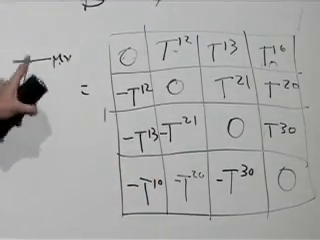
\includegraphics[width=0.82\textwidth]{lecture_06_figure_08.png}
\caption{一个完整的反对称\(4\times4\)阵列：对角线上为零，对角线两侧符号相反。}
\lectureframe{01:34:25}
\end{figure}

这个数目就是线索。三个电场分量和三个磁场分量可以放入一个反对称二阶张量中。

\section{电磁场张量}

让时空标签按\((1,2,3,0)=(x,y,z,t)\)的顺序横跨行和列。黑板上写出的排列是
\begin{equation}
  F_{\mu\nu}=
  \begin{pmatrix}
    0    & -B_3 & B_2  & E_1\\
    B_3  & 0    & -B_1 & E_2\\
    -B_2 & B_1  & 0    & E_3\\
    -E_1 & -E_2 & -E_3 & 0
  \end{pmatrix}.                                         \label{eq:l6-field-tensor}
\end{equation}
纯空间位置包含磁场；带有一个空间指标和一个时间指标的位置包含电场。一旦上三角矩阵元已知，反对称性就给出下三角矩阵元。

\begin{classroomqa}
\audiencequestion{磁场矩阵元是否全为负，并且标签是否对应于\(x,y,z\)？}
\lecturerresponse{上三角空间部分的符号如图所示交替：\(-B_3,+B_2,-B_1\)。标签\(1,2,3\)对应于\(x,y,z\)，而\(0\)标记时间。关于对角线反射会反转每个符号。}
\end{classroomqa}

\begin{figure}[H]
\centering
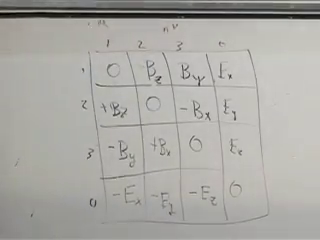
\includegraphics[width=0.82\textwidth]{lecture_06_figure_09.png}
\caption{按讲座中空间分量在前的分量顺序排列的完整电磁场张量。}
\lectureframe{01:41:05}
\end{figure}

按照惯例，这个记号写作\(F_{\mu\nu}\)，而不是一般的\(T_{\mu\nu}\)。讲师推测这个字母可能指法拉第，同时明确表示自己并不了解这一记号的历史。这里重要的是它的反对称性及其六个场分量，而不是关于这个字母的推测。

\begin{classroomqa}
\audiencequestion{矩阵的每个元素是否表示在所示坐标平面内的场的强度？}
\lecturerresponse{它是电磁场张量的一个分量。涉及时间的元素是电分量，而空间--空间元素则编码磁分量。}
\end{classroomqa}

把带有时间指标的列和行隔开。剩下的\(3\times3\)反对称块是磁性的。它的独立元素可以按循环方式记忆：
\begin{equation}
  F_{12}=-B_3,
  \qquad F_{23}=-B_1,
  \qquad F_{31}=-B_2.                                   \label{eq:l6-magnetic-cycle}
\end{equation}
从第一个关系式出发，让每个标号沿\(1\to2\to3\to1\)前进。等价地，
\begin{equation}
  F_{ij}=-\epsilon_{ijk}B_k,
\end{equation}
其中\(\epsilon_{123}=+1\)。\editorialnote{Levi--Civita公式就是黑板上明确展开的循环规则的紧凑标准形式。}

\begin{figure}[H]
\centering
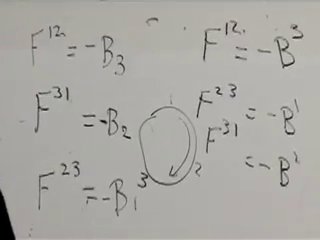
\includegraphics[width=0.82\textwidth]{lecture_06_figure_10.png}
\caption{反对称张量中编码磁场的循环空间分量。}
\lectureframe{01:46:20}
\end{figure}

电场的对应关系更为直接：
\begin{equation}
  E_1=F_{10},
  \qquad E_2=F_{20},
  \qquad E_3=F_{30}.
\end{equation}

因此磁场有两个有用的恒等式。在三维空间中，一个三分量的轴矢量可以与一个\(3\times3\)反对称张量配对。然而在时空中，它只是六分量张量\(F_{\mu\nu}\)的空间部分。这种配对是三维所特有的：一个反对称的\(4\times4\)张量有六个独立分量，不能与四维矢量等同。\editorialnote{在固有旋转下，磁场的行为像矢量；在反射下，更准确地说它是一个轴矢量，或赝矢量。}

这一构造的目的并不是为了数分量而数分量。因为\(F_{\mu\nu}\)按张量变换，洛伦兹助推会自动混合它的电分量和磁分量。在下一讲中，它可以与四维速度和四维加速度结合，用协变运动方程取代式~\eqref{eq:l6-lorentz-force}。

\section{关于爱因斯坦和闵可夫斯基的问题}

最后几分钟从形式体系转向它在历史上的起源。这些回答是作为回忆而非定论性的历史提供的，而这一限定本身就是交流的一部分。

\begin{classroomqa}
\audiencequestion{爱因斯坦是出于概念上的理由在寻求洛伦兹不变的表述，还是被特定的观测所驱动？}
\lecturerresponse{自然定律在每个惯性系中应具有相同形式这一原理是他推理的核心。此外还有关于光的实验证据以及未能探测到通过以太的运动，不过讲师明确表示不确定爱因斯坦知道哪些结果，或者这些结果对他有多大影响。概念上的压力在于，麦克斯韦方程组和洛伦兹力应当服从相对性原理，而这要求电场、磁场和速度分量一起变换。}
\end{classroomqa}

爱因斯坦1905年的表述并没有使用这里所用的紧凑四维矢量记号。它逐分量进行，把必要的\(\gamma\)因子和速度明确写出。闵可夫斯基随后把同样的结构几何化地组织为四维时空。

\begin{classroomqa}
\audiencequestion{爱因斯坦是否抵制闵可夫斯基的时空表述，闵可夫斯基又是在多久之后引入它的？}
\lecturerresponse{课堂上提供的回忆是，爱因斯坦起初并不欢迎四维几何语言，但很快采纳了它的价值。时间被暂定为1905年论文之后大约两年，也许是1907年；讲者强调他是在回忆而不是在确立历史。}
\end{classroomqa}

\begin{classroomqa}
\audiencequestion{闵可夫斯基是数学家还是物理学家，他还贡献了什么，他是否受到洛伦兹或菲茨杰拉德的影响？}
\lecturerresponse{并未声称有确定的答案。数学家和物理学家之间的区分没有被深究，一位听众的更正打断了关于闵可夫斯基其他工作的一段宽泛评论，而可能的影响线索被明确留作不确定。对于这次讨论而言，可靠的一点是闵可夫斯基以四维几何记号对相对性所作的决断性组织。}
\end{classroomqa}

\begin{classroomqa}
\audiencequestion{混合\(\boldsymbol E\)与\(\boldsymbol B\)的变换，在爱因斯坦1905年的工作中就已经出现了吗？}
\lecturerresponse{是的，但当时是逐分量写出的，而不是写成一个场张量方程。课堂上所作的对比是与麦克斯韦的分量方程的比较：内容可以在揭示其共同结构的紧凑记号出现之前就已经存在。闵可夫斯基的贡献在于使这一结构在时空语言中系统化。}
\end{classroomqa}

这就把我们带回了开头所提出的数学要点。分量对于计算是不可或缺的，但当这些分量被认识到是一个变换着的对象的各个部分时，定律才变得可以理解。接下来的任务是用\(F_{\mu\nu}\)把带电粒子的运动方程写成在每个惯性系中都相同的形式。

\chapter{带电粒子、场变换与相对论性波}

上次我们开始追问：一旦引入相对性原理，带电粒子在电场和磁场中如何运动。熟悉的洛伦兹力定律已经给出了线索：其磁力项依赖于粒子的速度，因此不同的观测者不可能分别就什么是电场、什么是磁场达成一致。我们的任务是重新表述这一定律，使得每个惯性观测者都使用同一个方程，尽管场和粒子速度会随参考系而改变。

除非另有说明，我们采用\(c=1\)的单位制，度规符号差为\((-,-,-,+)\)。时空分量的排列顺序是三个空间分量在前：
\begin{equation}
  \mu=(1,2,3,0)=(x,y,z,t).
\end{equation}
拉丁字母指标\(m,n\)只取三个空间方向。

\section{牛顿力定律中幸存下来的部分}

在牛顿力学中，
\begin{equation}
  \boldsymbol F=m\boldsymbol a
\end{equation}
在每个惯性系中都具有相同的形式，因为伽利略观测者对加速度的看法一致。他们也为粒子赋予相同的质量和力。一旦运动学发生改变，就没有理由期望力与普通加速度之间的这一特定关系保持不变。

电磁学和引力已经警告我们，相对论性的推广不必彼此相似。库仑定律和牛顿万有引力定律都是平方反比定律，但引力若不经过时空几何的更深层改变，就无法自然地纳入狭义相对论。电磁学则可以。事实上，磁性本身就是一种相对论效应：当恢复\(c\)的因子时，磁力带有速度除以\(c\)的因子，并在形式极限\(c\to\infty\)下消失。

牛顿定律中持久的部分是：力是动量的变化率。对于恒定的静止质量，
\begin{equation}
  \boldsymbol F
  =m\frac{d\boldsymbol v}{dt}
  =\frac{d}{dt}(m\boldsymbol v)
  =\frac{d\boldsymbol p}{dt}.
\end{equation}
相对论将改变动量与速度之间的关系，但会保留这种组织方程的方式。

\begin{figure}[H]
\centering
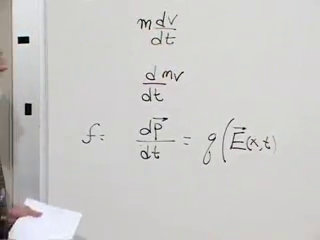
\includegraphics[width=0.64\textwidth]{lecture_07_figure_01.png}
\caption{当洛伦兹定律的电场部分被写在黑板上时，力被改写为\(d\boldsymbol p/dt\)。}
\lectureframe{00:08:20}
\end{figure}

在\(c=1\)的单位制下，前相对论性的洛伦兹力定律为
\begin{equation}
  \frac{d\boldsymbol p}{dt}
  =q\bigl(\boldsymbol E+\boldsymbol v\times\boldsymbol B\bigr).
  \label{eq:lorentz-three}
\end{equation}
两个场都可能依赖于位置和时间。非相对论极限现在是\(v\ll 1\)的极限，而不是数值常数\(c=1\)以某种方式发生改变的极限。\eqref{eq:lorentz-three}中的电场项已经是一个普通的矢量。为了以能够带入时空的形式理解磁力项，我们必须重新审视叉积。

\section{作为反对称张量的叉积}

取两个三维矢量\(\boldsymbol A\)和\(\boldsymbol B\)。它们的外积
\begin{equation}
  T_{mn}=A_mB_n
\end{equation}
是一个具有九个分量的二阶张量。它一般没有对称性。反对称化后得到
\begin{equation}
  K_{mn}=A_mB_n-A_nB_m,
  \qquad K_{mn}=-K_{nm}.
  \label{eq:antisym-product}
\end{equation}
其对角元为零，而对角线以下的每个元素都由其上方对应的元素确定。因此一个\(3\times3\)反对称张量只有三个独立分量。

这个计数具有启发性，但本身并不充分。三个量并不会自动像矢量那样变换。然而在三维中，\eqref{eq:antisym-product}的三个独立元素可以与叉积
\(\boldsymbol C=\boldsymbol A\times\boldsymbol B\)的分量等同起来。黑板首先将\(C_2\)临时放在右上位置：

\begin{figure}[H]
\centering
\includegraphics[width=0.75\textwidth]{lecture_07_figure_02.png}
\caption{反对称乘积，同时其三个独立元素正被与\(\boldsymbol C\)的分量进行匹配。右上角的标记在这里仍然是暂定的。}
\lectureframe{00:17:33}
\end{figure}

循环\(1\to2\to3\to1\)给出分量公式
\begin{align}
  C_3 &= A_1B_2-A_2B_1, \\
  C_1 &= A_2B_3-A_3B_2, \\
  C_2 &= A_3B_1-A_1B_3.
  \label{eq:cross-components}
\end{align}
最后一行表明右上角的元素是\(-C_2\)，而不是\(C_2\)。这一修正本身就是论证的一部分，而不是应当隐藏的细节。

\begin{figure}[H]
\centering
\includegraphics[width=0.62\textwidth]{lecture_07_figure_03.png}
\caption{完整的循环分量恒等式，它们确定了反对称阵列中临时符号。}
\lectureframe{00:21:54}
\end{figure}

由此得到的矩阵是
\begin{equation}
  K_{mn}=
  \begin{pmatrix}
    0 & C_3 & -C_2 \\
    -C_3 & 0 & C_1 \\
    C_2 & -C_1 & 0
  \end{pmatrix}.
  \label{eq:cross-matrix}
\end{equation}

这一记号背后有一个有用的几何图像。指标为\(1,2\)的分量自然属于\(xy\)平面，并被等同于沿垂直的\(z\)轴方向的矢量分量。人们可以用一个平面或用垂直于该平面的箭头来描述同一个有向对象。箭头的描述是三维所特有的；在更高维中，反对称二阶张量仍然存在，但其分量数目不再与矢量相同。因此，叉积得以推广的形式是张量，而不是垂直箭头。

等价地，选定一个定向之后，
\begin{equation}
  C_k=\frac12\epsilon_{kmn}K_{mn}.
\end{equation}
需要选定一个定向，这正是右手定则以及极矢量与轴矢量之间熟悉区别的来源。
\editorialnote{Levi--Civita 公式与轴矢量术语，是讲稿中明确展开的平面与法向几何的标准记号。}

\section{张量形式的磁场}

同样的对偶描述也适用于磁场。我们将其反对称空间张量定义为
\begin{equation}
  B_{mn}=
  \begin{pmatrix}
    0 & -B_3 & B_2 \\
    B_3 & 0 & -B_1 \\
    -B_2 & B_1 & 0
  \end{pmatrix}.
  \label{eq:magnetic-tensor}
\end{equation}
相对于 \eqref{eq:cross-matrix} 多出的整体符号是一个约定。
一旦选定，就必须一致地使用；改变全部三个矢量分量的符号，将以相反的定向约定描述同一个张量到矢量的等同。

\begin{figure}[H]
\centering
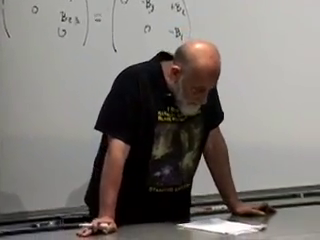
\includegraphics[width=0.72\textwidth]{lecture_07_figure_04.png}
\caption{磁场既写成反对称空间阵列，也用它三个矢量分量表示。}
\lectureframe{00:24:40}
\end{figure}

现在取叉积的第三个分量：
\begin{align}
  (\boldsymbol v\times\boldsymbol B)_3
  &=v_1B_2-v_2B_1 \\
  &=v_1B_{13}+v_2B_{23}+v_3B_{33}.
\end{align}
最后一项可以加上，因为 \(B_{33}=0\)。对自由分量进行轮换，得到紧凑规则
\begin{equation}
  (\boldsymbol v\times\boldsymbol B)_m=v_nB_{nm},
  \label{eq:cross-contraction}
\end{equation}
其中重复指标 \(n\) 被求和。因此磁力为
\begin{equation}
  F_m^{(B)}=qv_nB_{nm}.
\end{equation}

\begin{figure}[H]
\centering
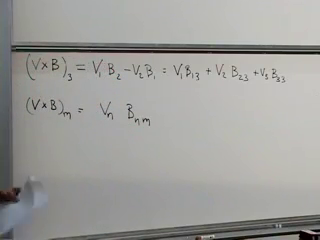
\includegraphics[width=0.78\textwidth]{lecture_07_figure_05.png}
\caption{\(\boldsymbol v\times\boldsymbol B\) 的第三个分量及其作为与 \(B_{nm}\) 缩并的一般表达式。}
\lectureframe{00:28:30}
\end{figure}

\begin{classroomqa}
\audiencequestion{自由指标 \(m\) 是否标记力的一个单独的磁分量？}
\lecturerresponse{不是。它标记的是正在计算的力的任意一个空间分量。为当前论证起见，电场已被简单地设为零，而这里的每个指标都只遍历三个空间方向。}
\end{classroomqa}

张量记号使磁场的无功性质几乎自动成立。对速率的平方求导：
\begin{align}
  \frac{d}{dt}(v_mv_m)
  &=2\dot v_m v_m \\
  &\propto 2(\boldsymbol v\times\boldsymbol B)_m v_m \\
  &=2v_nB_{nm}v_m.
  \label{eq:speed-derivative}
\end{align}
含 \(m=n\) 的项消失，因为 \(B_{nm}\) 的对角线为零。每个非对角项都有一个将 \(m\) 与 \(n\) 互换的配对项；二者相消，因为 \(v_nv_m\) 对称而 \(B_{nm}\) 反对称。
因此
\begin{equation}
  \frac{d}{dt}(v_mv_m)=0.
\end{equation}
纯磁力使轨迹弯曲，而不改变其速率或动能。

\begin{figure}[H]
\centering
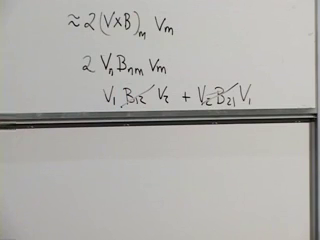
\includegraphics[width=0.68\textwidth]{lecture_07_figure_06.png}
\caption{\(v_nB_{nm}v_m\) 中的配对项相消，因为磁张量在交换其指标时改变符号。}
\lectureframe{00:35:40}
\end{figure}

这个证明有意比说叉积垂直于其第一个因子更为繁复。后一说法是三维矢量表示所特有的。对称对与反对称张量的缩并，才是将在四维中继续成立的论证。

\begin{classroomqa}
\audiencequestion{磁场是否必须与时间无关，速率才能保持恒定？}
\lecturerresponse{上述代数从未对场求导，也不要求 \(\partial_t\boldsymbol B=0\)。单独的磁项仍然不做功。然而在电动力学中，变化的磁场会产生电场，而该电场可以改变粒子的速率。}
\end{classroomqa}

\section{为什么电场与磁场必须混合}

在任何四维计算之前，就可以看出 \(\boldsymbol E\) 与 \(\boldsymbol B\) 的混合。考虑慢速运动，使得关于加速度的普通牛顿陈述足够。设磁场沿 \(y\) 轴，并设带电粒子沿 \(x\) 轴运动。磁力沿 \(z\) 轴：
\begin{equation}
  \boldsymbol F=q\boldsymbol v\times\boldsymbol B.
\end{equation}

\begin{figure}[H]
\centering
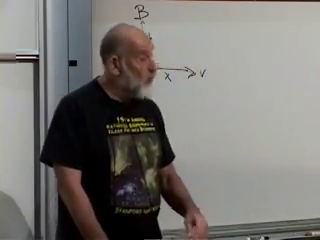
\includegraphics[width=0.62\textwidth]{lecture_07_figure_07.png}
\caption{粒子穿过磁场运动的板书草图；这三个方向用于比较实验室描述与共动描述。}
\lectureframe{00:42:20}
\end{figure}

可以不用教室的透视重新绘制该几何：
\begin{figure}[H]
\centering
\begin{tikzpicture}[scale=1.05,>=Stealth]
  \draw[->] (0,0) -- (3.8,0) node[right] {\(x\)};
  \draw[->] (0,0) -- (-1.9,2.4) node[above left] {\(y\)};
  \draw[->] (0,0) -- (0,3.1) node[above] {\(z\)};
  \draw[->,very thick] (0,0) -- (2.7,0)
    node[midway,below] {\(\boldsymbol v\)};
  \draw[->,very thick] (0,0) -- (-1.35,1.7)
    node[midway,above left] {\(\boldsymbol B\)};
  \draw[->,very thick] (0,0) -- (0,2.35)
    node[midway,right] {\(\boldsymbol F,\ \boldsymbol E'\)};
\end{tikzpicture}
\caption{在实验室中，沿 \(z\) 方向的力是磁力；在瞬时共动系中，同一个力必须是电力。}
\end{figure}

现在引入一个在该瞬间与粒子一起运动的观察者。粒子在新参考系中的速度为零，因此磁项 \(q\boldsymbol v'\times\boldsymbol B'\) 消失。然而在慢速运动极限下，两个观察者都必须同意粒子具有沿 \(z\) 的加速度。如果洛伦兹力定律在两个参考系中具有相同形式，那么共动观察者必须把该力归因于沿 \(z\) 的电场 \(\boldsymbol E'\)。因此，在实验室中纯为磁性的场，在运动参考系中并非纯为磁性。

这就是寻求一个其分量同时包含两种场的对象的物理原因。参考系的改变不只是让\(\boldsymbol E\)和\(\boldsymbol B\)各自的三个分量分别发生旋转；它还会混合这两组分量。

\section{电磁场张量}

电场和磁场合起来共有六个分量。一个四维反对称张量同样有六个独立分量，因为
\begin{equation}
  \frac{4(4-1)}{2}=6.
\end{equation}
这并不意味着反对称张量真的是人们所能构造出的唯一一种包含六个量的集合：六个标量，或者一个矢量加两个标量，也同样包含六个数。它是其分量能够以所需方式混合的自然几何客体。

为使板书约定明确，我们按空间分量在前的顺序\((1,2,3,0)\)写出逆变张量：
\begin{equation}
  F^{\mu\nu}=
  \begin{pmatrix}
    0 & -B_3 & B_2 & E_1 \\
    B_3 & 0 & -B_1 & E_2 \\
    -B_2 & B_1 & 0 & E_3 \\
    -E_1 & -E_2 & -E_3 & 0
  \end{pmatrix}.
  \label{eq:l07-field-tensor}
\end{equation}
左上角的\(3\times3\)分块正是磁张量\eqref{eq:magnetic-tensor}；带一个空间指标和一个时间指标的分量包含电场。反对称性给出了其余的元素。

\begin{figure}[H]
\centering
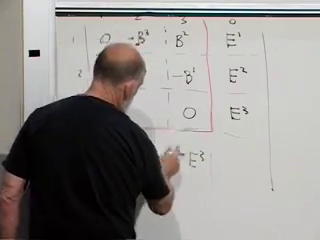
\includegraphics[width=0.72\textwidth]{lecture_07_figure_08.png}
\caption{磁性的空间分块与电性的时间-空间列被组装成四维场张量。}
\lectureframe{00:46:35}
\end{figure}

\begin{classroomqa}
\audiencequestion{这些场分量什么时候应当带上指标而不是下指标？}
\lecturerresponse{仅就三个空间标号而言，在辨认熟悉的麦克斯韦--法拉第场时，板书有时会略去这一区别。在协变计算中则必须恢复这一区别：在所选的度规约定下，升高或降低一个空间指标会改变一个符号。}
\end{classroomqa}

不变的不是板书上某种特定的符号排列，而是反对称的时空张量，连同自洽的度规与指标约定。记号\(F\)可能让人联想到法拉第，尽管本讲并不自信地主张这一历史归属。爱因斯坦在1905年给出了电场和磁场分量的变换；紧凑的四维张量语言则随着后来与闵可夫斯基相联系的时空表述而出现。

\section{四维速度与四维力}

方程中粒子一侧也必须协变化。固有时\(\tau\)是不变量，因此用它对位置四维矢量求导得到另一个四维矢量：
\begin{equation}
  u^\mu=\frac{dx^\mu}{d\tau}
  =\gamma(v_x,v_y,v_z,1),
  \qquad
  \gamma=\frac{1}{\sqrt{1-v^2}}.
  \label{eq:four-velocity}
\end{equation}
最后一个分量由\(dt/d\tau=\gamma\)得出。四维动量为
\begin{equation}
  p^\mu=mu^\mu,
\end{equation}
其空间部分就是相对论动量
\(\boldsymbol p=m\gamma\boldsymbol v\)。

\begin{figure}[H]
\centering
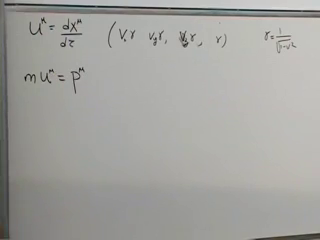
\includegraphics[width=0.75\textwidth]{lecture_07_figure_09.png}
\caption{四维速度、其分量、洛伦兹因子以及四维动量。}
\lectureframe{00:50:30}
\end{figure}

因为\(p^\mu\)是四维矢量而\(\tau\)是标量，自然的相对论性左端为
\begin{equation}
  f^\mu\equiv\frac{dp^\mu}{d\tau}.
  \label{eq:four-force-def}
\end{equation}
四维力不能任意选取。四维速度具有固定的模，
\begin{equation}
  u_\mu u^\mu=1.
\end{equation}
沿世界线求导给出
\begin{align}
  0
  &=\frac{d}{d\tau}(u_\mu u^\mu) \\
  &=\frac{du_\mu}{d\tau}u^\mu
    +u_\mu\frac{du^\mu}{d\tau} \\
  &=2u_\mu\frac{du^\mu}{d\tau}.
\end{align}
对于恒定质量，这意味着
\begin{equation}
  f^\mu u_\mu=0.
  \label{eq:force-orthogonal}
\end{equation}
因此四维力与四维速度闵可夫斯基正交。这是由\(u^\mu\)的归一化得出的纯运动学约束，而不是电磁学特有的性质。

\begin{figure}[H]
\centering
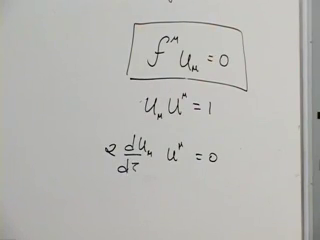
\includegraphics[width=0.64\textwidth]{lecture_07_figure_10.png}
\caption{四维速度的单位模以及由此得到的四维力与四维速度的正交性。}
\lectureframe{00:56:50}
\end{figure}

三维磁性的计算已经提供了满足\eqref{eq:force-orthogonal}的技巧。将一个反对称张量与速度的一份拷贝缩并：
\begin{equation}
  \boxed{
  \frac{dp^\mu}{d\tau}=qF^{\mu\nu}u_\nu.}
  \label{eq:covariant-lorentz}
\end{equation}
确实，
\begin{equation}
  f^\mu u_\mu
  =qF^{\mu\nu}u_\nu u_\mu=0,
\end{equation}
因为\(F^{\mu\nu}\)是反对称的而\(u_\nu u_\mu\)是对称的。这并不是唯一可能的相对论性力律，但它是对电磁场和速度都线性的最简单的一个。

\begin{figure}[H]
\centering
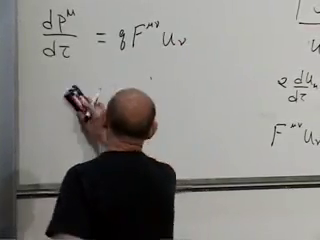
\includegraphics[width=0.72\textwidth]{lecture_07_figure_11.png}
\caption{左边是协变洛伦兹力方程，右边是它与第二个四维速度的缩并为零。}
\lectureframe{01:00:00}
\end{figure}

\section{恢复通常的洛伦兹力}

一个看似协变的方程仍必须重现已知的力律。按照开头所述的度规约定，
\begin{equation}
  u_\mu=\gamma(-v_x,-v_y,-v_z,1).
\end{equation}
对于\(x\)分量，\eqref{eq:l07-field-tensor}和\eqref{eq:covariant-lorentz}给出
\begin{align}
  \frac{dp^1}{d\tau}
  &=q\bigl(F^{12}u_2+F^{13}u_3+F^{10}u_0\bigr) \\
  &=q\gamma\bigl(B_3v_y-B_2v_z+E_1\bigr) \\
  &=q\gamma\bigl[\boldsymbol E+\boldsymbol v\times
    \boldsymbol B\bigr]_x.
  \label{eq:x-force}
\end{align}
其余空间分量可通过循环置换指标得到。

\begin{classroomqa}
\audiencequestion{分量展开中的\(qE_x\)项在哪里？}
\lecturerresponse{它就是\(qF^{10}u_0\)项。带一个空间指标和一个时间指标的场张量分量是电场分量，而\(u_0=\gamma\)。}
\end{classroomqa}

右端的因子\(\gamma\)并不是额外的力。由于
\begin{equation}
  \frac{dp^i}{d\tau}=\frac{dt}{d\tau}\frac{dp^i}{dt}
  =\gamma\frac{dp^i}{dt},
\end{equation}
它从\eqref{eq:x-force}的两端消去。因此精确的空间方程仍然是
\begin{equation}
  \frac{d\boldsymbol p}{dt}
  =q\bigl(\boldsymbol E+\boldsymbol v\times\boldsymbol B\bigr),
  \qquad
  \boldsymbol p=m\gamma\boldsymbol v.
  \label{eq:exact-three-force}
\end{equation}
熟悉的形式保留了下来，但相对论性隐藏在动量之中。

\begin{figure}[H]
\centering
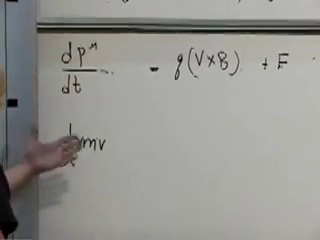
\includegraphics[width=0.75\textwidth]{lecture_07_figure_12.png}
\caption{去掉共同的固有时因子后，就恢复了三维洛伦兹定律；动量仍保留其\(\gamma\)因子。}
\lectureframe{01:06:30}
\end{figure}

时间分量承载着相应的能量陈述，
\begin{equation}
  \frac{dp^0}{dt}=q\boldsymbol E\cdot\boldsymbol v,
\end{equation}
因此磁场不做功，而电场可以改变粒子的能量。
\editorialnote{时间分量的检验是讲座中空间计算的直接对应部分；引入它是为了在四维记号中揭示同样的不做功性质。}

\begin{classroomqa}
\audiencequestion{这个推导是数学还是物理？}
\lecturerresponse{两者都是。张量代数提供了紧凑的形式，但实质性的物理内容是通过所有惯性系服从相同定律这一原理，以及运动方程为二阶这一假设进入的。二阶定律由位置和速度预测未来；三阶定律则需要把加速度作为额外的初始数据。是实验，而不是记号，告诉我们自然界使用哪一种定律。}
\end{classroomqa}

\section{场如何变换}

方程\eqref{eq:covariant-lorentz}在每个参考系中都具有相同的形式，因为两边都是四维矢量。场张量本身的变换则对每个指标各用一个洛伦兹矩阵：
\begin{equation}
  F'^{\mu\nu}
  =\Lambda^\mu{}_{\rho}\Lambda^\nu{}_{\sigma}F^{\rho\sigma}.
  \label{eq:tensor-transform}
\end{equation}
黑板上通过先变换一个简单的乘积\(A^\mu B^\nu\)来推导这条规则。一旦知道了矢量乘积的规则，线性性就给出了任意二阶张量的规则。

对于沿\(1\)轴的推动，坐标的变换为
\begin{align}
  x'^1&=\gamma(x^1-vx^0), &
  x'^0&=\gamma(x^0-vx^1), \\
  x'^2&=x^2, & x'^3&=x^3.
\end{align}
对两个张量指标分别施加同样的变换。对于平行于推动方向的分量，黑板从一个乘积开始：
\begin{align}
  (A'^0B'^1)
  =\gamma^2\bigl(
     A^0B^1-vA^0B^0-vA^1B^1+v^2A^1B^0
   \bigr).
\end{align}
把每个乘积替换为相应的张量分量，然后利用反对称性\(F^{00}=F^{11}=0\)和\(F^{10}=-F^{01}\)，得到
\begin{equation}
  F'^{01}
  =\gamma^2(1-v^2)F^{01}
  =F^{01}.
\end{equation}
因此平行于运动的电场分量不变。平行的磁场分量行为类似。

横向分量则不同。按照黑板上使用的带撇参考系和符号约定，
\begin{align}
  F'^{02}
  &=\gamma\bigl(F^{02}-vF^{12}\bigr), \\
  E'_2
  &=\gamma(E_2+vB_3).
  \label{eq:e-transform}
\end{align}
一个横向电场分量获得了一部分磁场分量。其余的变换定律由同样的双指标规则得出，留作讲座的练习。

\begin{figure}[H]
\centering
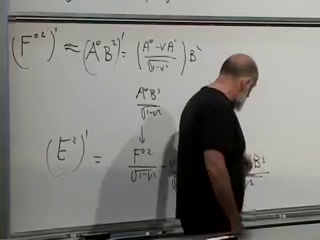
\includegraphics[width=0.76\textwidth]{lecture_07_figure_13.png}
\caption{在\(E'_2\)分量处，横向张量变换被看到包含一个正比于\(vB_3\)的项。}
\lectureframe{01:23:40}
\end{figure}

\eqref{eq:e-transform}中的符号取决于哪个参考系被声明为以\(+v\)运动，也取决于指标和度规约定。其不变内容则不取决于这些：横向电场和磁场分量相互混合，而变换之后协变力方程仍然成立。

\begin{classroomqa}
\audiencequestion{对于导线中的电流，能否以某个速度运动从而使磁场消失？}
\lecturerresponse{随传导电子一起运动是不够的，因为这样一来正晶格电荷就在新参考系中运动了。因此，一条中性的载流导线比单个运动的电荷团更微妙。纯磁场不能被完全变换掉。如果电场和磁场同时存在，它们的变换部分在特殊情况下可以相消；对于单个匀速运动的电荷，电荷的静止系就是使其磁场消失的简单参考系。}
\end{classroomqa}

精确的不变判据使用
\begin{equation}
  \boldsymbol B^2-\boldsymbol E^2,
  \qquad
  \boldsymbol E\cdot\boldsymbol B.
\end{equation}
只有当电场占主导且\(\boldsymbol E\cdot\boldsymbol B=0\)时，才可能存在满足\(\boldsymbol B'=0\)的参考系；在一个参考系中为纯磁场的场是磁场占主导的，不能满足该条件。
\editorialnote{这些不变判据精确地陈述了课堂讨论中得到的限定条件；它们的推导被推迟。}

\begin{classroomqa}
\audiencequestion{电标势和磁矢势构成一个四维矢量吗？}
\lecturerresponse{是的。在依赖于约定的符号下，它们组合成四维势\(A^\mu\)。麦克斯韦方程组将系统地使用这个对象。}
\end{classroomqa}

\section{场的导数}

现在我们离开单个粒子的轨迹，考虑遍布时空的场。设
\begin{equation}
  \phi=\phi(x^1,x^2,x^3,x^0)
\end{equation}
为一个标量场。它的四个导数构成一个四维矢量的协变分量：
\begin{equation}
  \partial_\mu\phi
  \equiv\frac{\partial\phi}{\partial x^\mu}
  =\left(
    \frac{\partial\phi}{\partial x},
    \frac{\partial\phi}{\partial y},
    \frac{\partial\phi}{\partial z},
    \frac{\partial\phi}{\partial t}
  \right).
\end{equation}
对洛伦兹坐标变换应用链式法则，就证明了这条协变变换定律。升高指标会反转空间符号，但时间符号保持不变：
\begin{equation}
  \partial^\mu\phi
  =\left(
    -\frac{\partial\phi}{\partial x},
    -\frac{\partial\phi}{\partial y},
    -\frac{\partial\phi}{\partial z},
    \frac{\partial\phi}{\partial t}
  \right).
\end{equation}

每一次微分都会贡献一个下指标。因此，\(\partial_\nu V^\mu\) 是一个具有一个上指标和一个下指标的二阶张量，而对张量求导会产生一个额外多出一个下指标的对象。这就是在不选择任何优先惯性系的情况下写出场方程所需的基本规则。

\section{不变标量波动方程}

最简单的波动方程包含两个导数。如果该方程要在每个惯性系中都具有相同形式，其左侧就应当是一个标量。对导数指标进行缩并，得到唯一最简单的选择：
\begin{equation}
  \boxed{\partial^\mu\partial_\mu\phi=0.}
  \label{eq:wave-covariant}
\end{equation}
在当前号差下写出其分量，
\begin{equation}
  \frac{\partial^2\phi}{\partial t^2}
  -\frac{\partial^2\phi}{\partial x^2}
  -\frac{\partial^2\phi}{\partial y^2}
  -\frac{\partial^2\phi}{\partial z^2}=0.
  \label{eq:wave-components}
\end{equation}
\eqref{eq:wave-covariant} 中的缩并使洛伦兹不变性显而易见；方程 \eqref{eq:wave-components} 则是同一陈述按分量逐项写出的形式。

\begin{figure}[H]
\centering
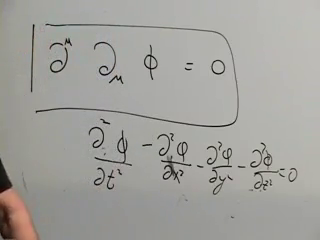
\includegraphics[width=0.75\textwidth]{lecture_07_figure_14.png}
\caption{标量波动方程的缩并导数形式及其时间减空间的分量展开。}
\lectureframe{01:39:40}
\end{figure}

\begin{classroomqa}
\audiencequestion{波动方程的右侧必须为零吗？}
\lecturerresponse{不。它可以是任何与问题相容的标量。一个常数乘以 \(\phi\)，或者一个非线性标量函数，例如与 \(\phi^2\) 成正比的函数，仍然保持协变性。取零则给出最简单的自由波动方程。}
\end{classroomqa}

这个标量示例的意义在于作准备。麦克斯韦方程组以更复杂的方式混合电场和磁场，但它们同样可以被写成使其洛伦兹不变性从指标结构中显而易见的形式。这就是我们下次要回到的问题。
\chapter{度规、膨胀与最初的宇宙学}

在前一讲的末尾，我们已经得到了一个洛伦兹不变的波动方程，并正准备把麦克斯韦方程组写成时空形式。现在，在转向引力之前，一位听众的提问提供了一个有用的警示：对称性本身究竟能决定一个物理理论的多少内容？答案是明确的：能决定很多，但并非全部。洛伦兹不变性是对可能定律的一个强有力的筛选条件。它并不能替代其余物理假设，也不能替代实验。

\section{对称性所不能决定的内容}

\begin{classroomqa}
\audiencequestion{一旦已知电场和磁场在洛伦兹变换下会一起变换，麦克斯韦方程组是否仅由相对论就能推出？}
\lecturerresponse{不能。相对论约束了这些方程的形式，但其构造还使用了方程的线性性、其导数阶数之低、场变换的方式以及实验信息。若没有这些额外要素，许多洛伦兹协变的场方程仍将是可能的。}
\end{classroomqa}

在开篇讨论中，这些额外假设里最重要的是线性性。如果\(A(x,t)\)是某个线性场方程的解，那么对任意常数\(\lambda\)，\(\lambda A(x,t)\)也是解。如果\(A\)和\(B\)是解，那么\begin{equation}
  C(x,t)=A(x,t)+B(x,t).
  \label{eq:superposition}
\end{equation}也是解。这就是叠加原理。两列无源电磁波可以彼此交叉而保持原样。它们不会像实物那样直接碰撞。它们可以通过带电物质间接相互作用，因为每一列波都会推动电荷，而运动电荷会辐射，但真空中的场方程本身是线性的。

\begin{figure}[H]
\centering
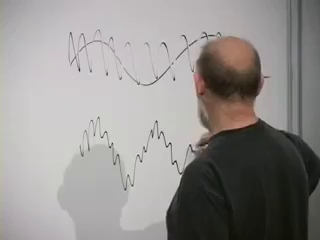
\includegraphics[width=0.64\textwidth]{lecture_08_figure_01.png}
\caption{讨论叠加原理时黑板上的两个波剖面。它们的和仍然是一列允许的无源波。}
\lectureframe{00:05:30}
\end{figure}

谐振子使这套代数变得清楚明了。假设\begin{equation}
  m\ddot x=-kx.
  \label{eq:linear-oscillator}
\end{equation}。如果\(x_1\)和\(x_2\)解\eqref{eq:linear-oscillator}，那么\begin{equation}
  m(\ddot x_1+\ddot x_2)
  =-k(x_1+x_2),
\end{equation}，所以\(x_1+x_2\)是解。然而，加上一个非线性项后，\begin{equation}
  m\ddot x=-kx+p x^2,
  \label{eq:nonlinear-oscillator}
\end{equation}，其和就不再成立：\begin{equation}
  (x_1+x_2)^2=x_1^2+x_2^2+2x_1x_2.
\end{equation}。交叉项\(2x_1x_2\)在两个分开的方程中没有对应项。这两种运动现在会相互影响。

\begin{figure}[H]
\centering
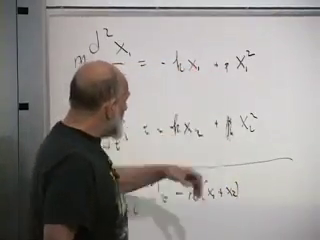
\includegraphics[width=0.73\textwidth]{lecture_08_figure_02.png}
\caption{将分开的振子方程与其和的方程相比较。二次项暴露出破坏叠加原理的额外交叉项。}
\lectureframe{00:10:10}
\end{figure}

这个例子确定了将在整个宇宙学讨论中始终有效的方法论要点。对称性告诉我们哪些量可以组合，以及哪些方程是允许的。动力学和观测则告诉我们自然界使用的是哪一个允许的方程。

\section{作为几何的间隔}

现在我们离开电磁学，走一条短路线进入广义相对论和宇宙学。起始对象是相邻事件之间的间隔。用一个四维坐标\(x^\mu\)标记一个事件，并用\(x^\mu+dx^\mu\)标记一个邻近事件。在惯性笛卡儿坐标中，取\(c=1\)和\((+,-,-,-)\)约定，\begin{equation}
  d\tau^2
  =dt^2-dx^2-dy^2-dz^2
  =dx^\mu dx_\mu
  =\eta_{\mu\nu}\,dx^\mu dx^\nu.
  \label{eq:minkowski-interval}
\end{equation}。不变量是量\(d\tau^2\)，而不是任何一个坐标差。洛伦兹变换会改变\(dt,dx,dy,dz\)，同时保持这个二次组合不变。因此，狭义相对论可以被解读为闵可夫斯基时空的几何。

\begin{figure}[H]
\centering
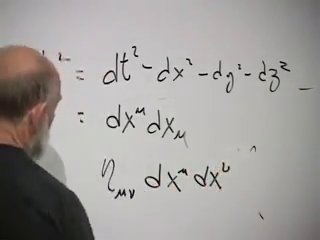
\includegraphics[width=0.72\textwidth]{lecture_08_figure_03.png}
\caption{闵可夫斯基间隔依次用分量、缩并指标和度规张量记号写出。}
\lectureframe{00:14:50}
\end{figure}

\eqref{eq:minkowski-interval}的简单性取决于坐标。即使是一个平坦平面，如果我们不明智地给它标记坐标，也会获得不熟悉的系数。设\(x\)以厘米为单位测量，而\(y\)以米为单位测量。对于一个物理位移，\begin{equation}
  ds^2=dx^2+\left(\frac{dy}{100}\right)^2
      =dx^2+10^{-4}dy^2.
  \label{eq:mixed-units}
\end{equation}。因子\(10^{-4}\)与曲率毫无关系。它只是在单位之间进行换算。

\begin{figure}[H]
\centering
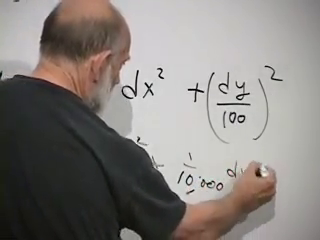
\includegraphics[width=0.59\textwidth]{lecture_08_figure_04.png}
\caption{一个平坦平面，一个轴用厘米描述，另一个轴用米描述。不相等的度规系数编码的是单位，而不是曲率。}
\lectureframe{00:20:10}
\end{figure}

斜坐标会添加一个混合项。在二维中，最一般的局部二次型可以写成\begin{align}
  ds^2
  &=a_{11}\,dx^2+a_{12}\,dx\,dy\notag\\
  &\quad+a_{21}\,dy\,dx+a_{22}\,dy^2,
  \qquad a_{12}=a_{21}.
  \label{eq:quadratic-form}
\end{align}。因为普通微分可交换，\(dx\,dy=dy\,dx\)，所以只有系数阵列的对称部分有贡献。我们把系数收集到矩阵\begin{equation}
  g=
  \begin{pmatrix}
    a_{11} & a_{12}\\
    a_{21} & a_{22}
  \end{pmatrix}.
  \label{eq:metric-matrix}
\end{equation}中。这个矩阵就是\emph{度规}。它是把坐标差转换为物理间隔的局部规则。

\begin{figure}[H]
\centering
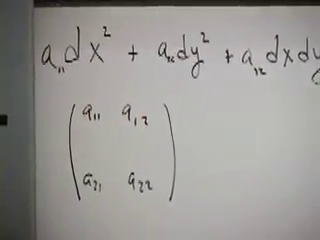
\includegraphics[width=0.71\textwidth]{lecture_08_figure_05.png}
\caption{二次微分形式及其对称的\(2\times2\)系数矩阵，此时该矩阵被认定为度规。}
\lectureframe{00:24:07}
\end{figure}

均匀的矩形或斜交网格给出常系数。如果坐标线弯曲、聚拢或散开，那么即使底层曲面仍然是平的，这些系数也会变成位置的函数。一般的时空记号是
\begin{equation}
  ds^2=g_{\mu\nu}(x)\,dx^\mu dx^\nu.
  \label{eq:general-metric}
\end{equation}

\begin{figure}[H]
\centering
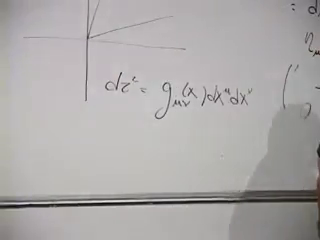
\includegraphics[width=0.66\textwidth]{lecture_08_figure_06.png}
\caption{允许坐标网格逐点变化后的一般位置依赖度规。}
\lectureframe{00:28:10}
\end{figure}

在指定坐标系中知道\(g_{\mu\nu}\)，就确定了局部的距离、时间和角度，从而确定了几何。反之则不唯一：一种几何有无穷多种坐标描述，因此有无穷多组由坐标变换相联系的系数函数阵列。

\section{坐标复杂性与内禀曲率}

我们现在必须把复杂的度规与弯曲的空间区分开来。把一张纸卷成圆柱而不拉伸它。它在房间中的外观改变了，但在纸内测得的所有距离都保持不变。一个被限制在纸上的生物无法通过任何内禀测量探测到这种弯曲。那是外在弯曲，不是这里所说的曲率。

半球则不同。不拉伸、不撕裂、不压缩它，就无法把它压平。地球的平面地图必然扭曲距离、面积、角度或它们的某种组合。这种阻碍是内禀的，无需看向周围维度就能探测到。

极坐标给出了不可或缺的平坦反例。在平面上，无穷小径向位移的长度为\(dr\)，而在半径\(r\)处的角位移\(d\theta\)的长度为\(r\,d\theta\)。因此
\begin{equation}
  ds^2=dr^2+r^2d\theta^2,
  \qquad
  g_{\text{polar}}=
  \begin{pmatrix}
    1&0\\
    0&r^2
  \end{pmatrix}.
  \label{eq:polar-metric}
\end{equation}
系数\(r^2\)在整个平面上变化，然而平面是平的。变量变换
\begin{equation}
  x=r\cos\theta,\qquad y=r\sin\theta
\end{equation}
又回到常度规\(ds^2=dx^2+dy^2\)。

\begin{figure}[H]
\centering
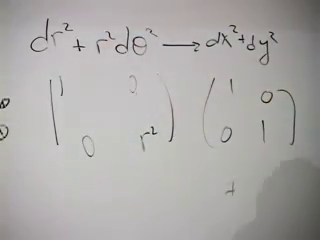
\includegraphics[width=0.70\textwidth]{lecture_08_figure_07.png}
\caption{极坐标度规及其向笛卡尔度规的回归。左边位置依赖的矩阵仍然描述一个平坦的平面。}
\lectureframe{00:39:20}
\end{figure}

\begin{classroomqa}
\audiencequestion{极坐标中的角距离是否应包含一个正弦？}
\lecturerresponse{在平面上不是。那里的弧长是\(r\,d\theta\)。正弦出现在球面上，那里一条纬线圆的半径为\(R\sin\theta\)。}
\end{classroomqa}

取半径为\(R\)的球面。设\(\theta\)为从北极量起的极角，\(\phi\)为方位角。经向一步的长度为\(R\,d\theta\)。在极角\(\theta\)处，纬圈的半径为\(R\sin\theta\)，因此方位角一步的长度为
\(R\sin\theta\,d\phi\)。局部勾股定理给出
\begin{align}
  ds^2
  &=R^2\left(d\theta^2+\sin^2\theta\,d\phi^2\right),
  \label{eq:sphere-metric}\\
  g_{\text{sphere}}=
  &\begin{pmatrix}
    R^2&0\\
    0&R^2\sin^2\theta
  \end{pmatrix}.
\end{align}

\begin{figure}[H]
\centering
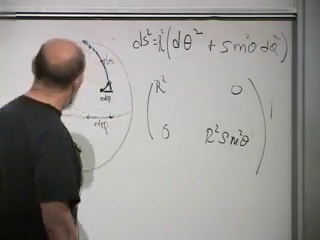
\includegraphics[width=0.72\textwidth]{lecture_08_figure_08.png}
\caption{球面、其角向线元以及相应的度规矩阵。\(\sin^2\theta\)因子记录了纬圈的收缩。}
\lectureframe{00:45:15}
\end{figure}

\begin{figure}[H]
\centering
\begin{tikzpicture}[scale=1.05]
  \draw (0,0) circle (2.1);
  \draw[dashed] (-2.1,0) arc (180:360:2.1 and 0.52);
  \draw (2.1,0) arc (0:180:2.1 and 0.52);
  \coordinate (P) at (48:2.1);
  \fill (P) circle (1.5pt);
  \draw (0,0) -- (0,2.1);
  \draw (0,0) -- (P);
  \draw (0,0.82) arc (90:48:0.82);
  \node at (0.47,1.03) {\(\theta\)};
  \draw[->] (P) -- ++(-0.34,0.36)
    node[midway,left] {\(R\,d\theta\)};
  \draw[->] (P) -- ++(0.76,0)
    node[midway,above] {\(R\sin\theta\,d\phi\)};
\end{tikzpicture}
\caption{用于得到\eqref{eq:sphere-metric}的局部微分腿的清晰重构。}
\end{figure}

没有任何整体坐标变换能把\eqref{eq:sphere-metric}变成常欧几里得矩阵。一个二维观测者可以内禀地发现这一点：由测地线构成的足够大的三角形，其内角和大于\(180^\circ\)。因此我们得到了有用的判据。变系数本身并不蕴含曲率。曲率是找不到使度规在所考虑区域内处处为常数的坐标这一阻碍。

\section{从弯曲时空到宇宙学}

广义相对论允许时空本身具有这种内禀曲率。位置依赖的\(g_{\mu\nu}\)可能仍然只是坐标的产物，如在极坐标中那样，但在真正弯曲的时空中，没有任何坐标变换能在整体上消除这种变化。

\begin{figure}[H]
\centering
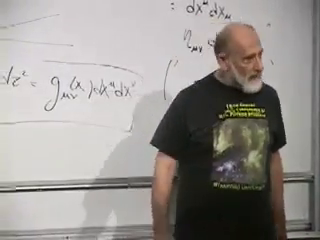
\includegraphics[width=0.70\textwidth]{lecture_08_figure_09.png}
\caption{从特殊坐标例子到一般时空线元\(ds^2=g_{\mu\nu}(x)dx^\mu dx^\nu\)的过渡。}
\lectureframe{00:48:40}
\end{figure}

我们不会尝试爱因斯坦方程的全部机器。相反，我们把注意力限制在适合宇宙学的几何上：空间在足够大的尺度上被取为均匀的，而几何可以随时间变化。均匀意味着没有任何位置与其他位置相区别。它并不意味着平坦：球面上的每一点都等价，然而球面是弯曲的。它也不意味着在每个尺度上都无特征。

\begin{classroomqa}
\audiencequestion{如果星系会形成星系团、片状结构和纤维状结构，宇宙怎么可能是均匀的？}
\lecturerresponse{这一论断涉及的是粗粒化尺度。恒星、星系和星系团是强烈非均匀的。当把横跨数亿光年的区域相互比较时，这些结构在平均意义上趋于均匀分布。宇宙学原理是一种经验性的工作假设，而不是逻辑上的必然；足够大的系统性差异，包括宇宙背景中的方向性差异，都可能证伪它。}
\end{classroomqa}

本讲的第二个大尺度假设是空间平坦性。在固定的宇宙时刻，足够大的三角形看起来是欧几里得的：其内角之和为\(180^\circ\)。这是关于三维空间几何的陈述，尚未涉及四维时空的曲率。

\begin{classroomqa}
\audiencequestion{对于相隔宇宙学距离的点，同时性意味着什么？毕竟它们的光在不同时刻到达我们这里。}
\lecturerresponse{我们无法在遥远星系之间放置量杆，也无法瞬时地检视它们。我们是在较晚的时候接收到信号，并在某个时空模型内重建发射事件的几何。这一程序是间接的，但天文学中的许多几何测量也是如此。平坦性意味着，在所考察的尺度上，重建出的大三角形没有可探测到的角盈余或角亏损。}
\end{classroomqa}

\section{共动坐标与尺度因子}

想象一张笛卡尔网格被画在星系的大尺度流动之上。随着网格膨胀，每个星系保持其坐标标签不变。这个标签不是以米为单位的距离，而是一个地址。一个随时间变化的转换因子把坐标间隔变成物理间隔。

\begin{figure}[H]
\centering
\begin{tikzpicture}[>=Latex,scale=0.86]
  \foreach \x in {0,0.65,1.3,1.95,2.6} {
    \draw[gray!65] (\x,0) -- (\x,2.2);
  }
  \foreach \y in {0,0.55,1.1,1.65,2.2} {
    \draw[gray!65] (0,\y) -- (2.6,\y);
  }
  \fill[blue!65!black] (0.65,0.55) circle (2pt);
  \fill[red!70!black] (1.95,1.65) circle (2pt);
  \node[below] at (1.3,-0.2) {comoving labels at \(t_1\)};
  \draw[->,very thick] (3.0,1.1) -- (4.0,1.1)
    node[midway,above] {\(a(t)\) grows};
  \foreach \x in {4.4,5.5,6.6,7.7,8.8} {
    \draw[gray!65] (\x,0) -- (\x,2.2);
  }
  \foreach \y in {0,0.55,1.1,1.65,2.2} {
    \draw[gray!65] (4.4,\y) -- (8.8,\y);
  }
  \fill[blue!65!black] (5.5,0.55) circle (2pt);
  \fill[red!70!black] (7.7,1.65) circle (2pt);
  \node[below] at (6.6,-0.2) {same labels at \(t_2\)};
\end{tikzpicture}
\caption{共动地址保持固定，而坐标网格的物理间距在增大。}
\end{figure}

空间均匀性要求：在给定时刻，处处都有相同的转换因子。空间平坦性则允许度规的空间部分取笛卡尔形式。由此得到的线元为
\begin{equation}
  d\tau^2
  =dt^2-a^2(t)\left(dx^2+dy^2+dz^2\right).
  \label{eq:flrw-flat}
\end{equation}
这就是共动坐标下空间平坦的均匀宇宙学度规。我们可以选择让\(x,y,z\)无量纲，并赋予\(a(t)\)长度的单位。另一种约定可以把量纲放进坐标中，使\(a\)无量纲；只有乘积才是有意义的。

\begin{figure}[H]
\centering
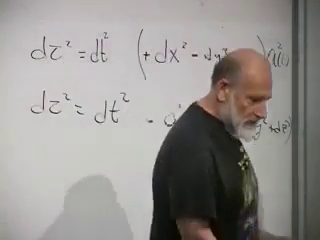
\includegraphics[width=0.76\textwidth]{lecture_08_figure_10.png}
\caption{黑板上写出的空间平坦宇宙学度规，其中共同的因子\(a^2(t)\)乘在全部三个空间方向上。}
\lectureframe{01:03:15}
\end{figure}

如果\(a\)是常数，我们就可以通过重新标度\(x,y,z\)把它吸收掉，而\eqref{eq:flrw-flat}就会是换用不同单位的普通闵可夫斯基时空。它的时间依赖才是非平凡之处。

\begin{classroomqa}
\audiencequestion{如果坐标网格在膨胀，为什么米尺、原子和星系不随之膨胀？}
\lecturerresponse{度规描述的是宇宙的平均流动，而不是一种迫使每个束缚系统都跟随它的力。电磁力把米尺和原子束缚在一起；自引力把星系束缚在一起。在小尺度上，这些束缚效应压倒了极其微弱的背景膨胀。近邻星系也可以偏离哈勃流：仙女座星系正被银河系吸引。对星系束缚的详细研究表明，仅有可见物质是不够的，这是支持暗物质的论据之一。}
\end{classroomqa}

\begin{classroomqa}
\audiencequestion{为什么尺度因子本身不是一种把星系推开的力？}
\lecturerresponse{在目前的约定下，它具有长度的量纲，而不是力的量纲。想想向上发射的一颗炮弹。一旦发射出去，它的向外运动就是惯性的；引力通过减小其速度或把它拉回来来改变这种运动。同样，膨胀是一种运动状态。动力学问题是引力和其它源如何改变\(\dot a\)和\(\ddot a\)，而不是需要什么力来维持\(a\)的运动。}
\end{classroomqa}

过去的预期是，吸引性引力应当使膨胀减速。到本讲之时，天文证据已经表明，近期的膨胀反而在加速，这意味着完整的动力学所包含的内容不止普通的吸引性物质。我们把这个问题推迟到几何框架稳固之后再讨论。

\section{哈勃定律}

取两个共动星系，其固定坐标间隔为
\(\Delta x\)。在共同的宇宙时刻，它们的物理距离为
\begin{equation}
  D(t)=a(t)\,\Delta x.
  \label{eq:physical-distance}
\end{equation}
在保持共动标签固定的情况下求导：
\begin{align}
  V(t)
    &=\dot D(t)
      =\dot a(t)\,\Delta x \nonumber\\
    &=\frac{\dot a(t)}{a(t)}D(t).
  \label{eq:hubble-derivation}
\end{align}
定义
\begin{equation}
  H(t)=\frac{\dot a(t)}{a(t)}.
  \label{eq:hubble-parameter}
\end{equation}
于是
\begin{equation}
  V(t)=H(t)D(t).
  \label{eq:hubble-law}
\end{equation}
在某一宇宙时刻，同一个\(H(t)\)处处适用；否则空间就不会是均匀的。退行速度与距离成正比，因为共动网格中的每一个间隔都以相同的分数速率被拉伸。

\begin{figure}[H]
\centering
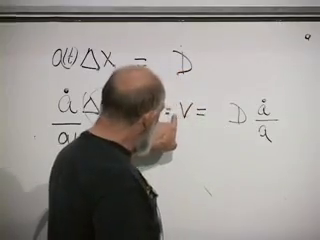
\includegraphics[width=0.73\textwidth]{lecture_08_figure_11.png}
\caption{物理距离\(D=a\Delta x\)及其时间导数，在通向\(V=(\dot a/a)D\)的过程中。}
\lectureframe{01:16:45}
\end{figure}

\begin{classroomqa}
\audiencequestion{对于一个遥远的星系，哈勃参数应当用现在的值，还是用所观测到的光发出时的值来求？}
\lecturerresponse{用所描述的那个时期的值。来自遥远星系的光报告的是较早的膨胀值。严肃的分析必须考虑\(H\)的时间依赖性；处处代入今天的值只是一种局部近似。}
\end{classroomqa}

\begin{classroomqa}
\audiencequestion{在\(D=a\Delta x\)中，单位存在于何处？}
\lecturerresponse{一个方便的选择是把共动标签\(\Delta x\)视为无量纲，而让\(a\)带有长度量纲。相反的记账方式也是可能的。无论哪种方式，\(H=\dot a/a\)都具有时间的倒数量纲。}
\end{classroomqa}

\section{膨胀坐标中的光}

光沿零路径传播。沿这样的路径，固有时间隔为零：
\begin{equation}
  d\tau^2=0.
\end{equation}

\begin{classroomqa}
\audiencequestion{为什么光的间隔为零？}
\lecturerresponse{这就是相对论中光线之所以为光线的定义性几何。每一个局部自由下落的观测者都测得光以\(c=1\)运动，因此局部地有\(dt^2=d\ell^2\)，时空间隔为零。这并不意味着接收光的观测者没有坐标时间流逝。}
\end{classroomqa}

对于只沿\(x\)方向运动的光线，
\begin{equation}
  0=dt^2-a^2(t)\,dx^2.
\end{equation}
选择朝\(x\)增大的方向运动的那条光线，
\begin{equation}
  dt=a(t)\,dx,
  \qquad
  dx=\frac{dt}{a(t)},
  \qquad
  \frac{dx}{dt}=\frac{1}{a(t)}.
  \label{eq:null-ray}
\end{equation}

\begin{figure}[H]
\centering
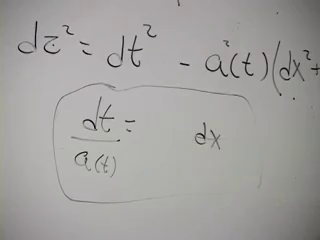
\includegraphics[width=0.64\textwidth]{lecture_08_figure_12.png}
\caption{膨胀度规中的零条件以及由此得到的共动光线方程\(dx=dt/a(t)\)。}
\lectureframe{01:23:45}
\end{figure}

坐标速度\(dx/dt\)随尺度因子增大而减小。这并不意味着光在局部变慢。一个单位的共动坐标距离代表越来越大的物理距离，因此坐标速度的数值发生变化，而每一次局部测量仍然给出\(c=1\)。

\section{为什么时间依赖性很重要}

现在，核心的几何问题不可避免：\(a(t)\)如何变化？类比于一个在某时刻位置已知的抛射体。它未来的轨迹需要运动方程。在宇宙学中，引力动力学将提供关于\(a(t)\)的方程。

\begin{classroomqa}
\audiencequestion{为什么要特别追问\(a(t)\)是否随时间变化，而不去同样合理地追问例如电子电荷是否随时间变化？}
\lecturerresponse{并不存在逻辑上的等级之分。电子电荷若被测出变化，那将是极其重要的。我们聚焦于\(a(t)\)，是因为观测已经告诉我们宇宙间隔在变化，而电子电荷看起来是恒定的。从几何上看，一个恒定的\(a\)可以通过改变空间单位而被移除，并留下平坦时空；一个随时间变化的\(a\)则不能以那种方式被移除。}
\end{classroomqa}

在测量遥远星系的退行之前，需要这个几何框架来说明所测量的究竟是什么。在最粗略的层面上，一个已知光度的源会因距离而显得更暗，因为它的光散布在更大的面积上；而已知原子谱线的位移给出红移，从而给出退行指标。哈勃把距离估计与红移结合起来，揭示了正比关系
\eqref{eq:hubble-law}，尽管该系数早期的数值有实质性错误。现代的距离阶梯和相对论性光传播计算要精细得多，但概念上的配对仍然是距离加红移。

\section{哈勃时间与年龄估计}

哈勃定律中隐藏着一个简单的估计。冻结一个星系当前的退行速度，并让运动均匀地反向进行。闭合其当前距离所需的时间将是
\begin{equation}
  t=\frac{D}{V}.
\end{equation}
利用\(V=HD\)，
\begin{equation}
  t=\frac{D}{HD}=\frac{1}{H}.
  \label{eq:hubble-time}
\end{equation}
距离被消去，因此每一对共动星系都给出相同的粗略时间。Susskind在此抓住并纠正了一个容易犯的措辞错误。假设并不是\(H\)保持恒定。而是把那个特定的退行速度当作恒定的一样向后外推。

\begin{figure}[H]
\centering
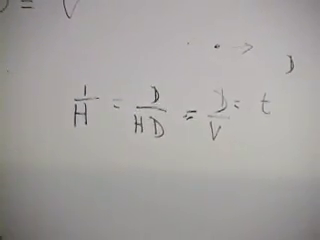
\includegraphics[width=0.66\textwidth]{lecture_08_figure_13.png}
\caption{哈勃时间估计 \(H^{-1}=D/(HD)=D/V\)，其中距离在反向外推中相消。}
\lectureframe{01:33:45}
\end{figure}

因此，逆哈勃参数是一个时间尺度，并不自动等于宇宙的精确年龄。在纯减速、物质主导的图像中，将当前速度反向，并让引力把星系拉回到一起。它们相遇的时间比在匀速情况下更早，所以当前的 \(H^{-1}\) 高估了年龄。讲座引用了一个更精确的年龄，约为 \(13.5\) 亿年，接近哈勃时间但并不完全相同。

\begin{classroomqa}
\audiencequestion{如果我们的星系内部没有哈勃膨胀，那么把所有星系反向运行直到它们坍缩意味着什么？}
\lecturerresponse{均匀描述最终不再能分辨束缚结构的真实历史。在时间正向上，小涨落通过引力增长为星系和星系团。字面意义上的倒放电影将要求每一个微观运动都反向，并且熵减少；仅仅反转平均哈勃流并不能撤销结构形成。反向外推是一种粗略的宇宙学估计，而不是每颗恒星沿其路径回溯的影片。}
\end{classroomqa}

\begin{classroomqa}
\audiencequestion{实验能否区分星系际距离在膨胀与尺子在收缩？}
\lecturerresponse{只有无量纲比值是可观测的。所测量到的是星系之间的距离除以原子或实验室长度标准后增大。我们习惯上保持原子和分子物理的参数固定，并说宇宙在膨胀。也可以选择星系际间距作为标准，而把原子、质子和米尺描述为在收缩。该比值的物理将保持不变。}
\end{classroomqa}

这种约定是自然的，因为尺子由原子构成，而其大小由那些看起来恒定的参数控制。一米归根结底是大量微观长度的总和。保持这些微观标准固定，就得到熟悉的说法：\(a(t)\) 在增长。

\begin{classroomqa}
\audiencequestion{\eqref{eq:flrw-flat} 是唯一与空间均匀性和平坦性相容的度规吗？}
\lecturerresponse{只在坐标变换的意义下唯一。精确的说法是，在这些假设下，并适当选择宇宙时间和共动空间坐标，度规可以被化为这种形式。另一个坐标系可能使同一个时空看起来相当不同。}
\end{classroomqa}

\begin{classroomqa}
\audiencequestion{当反向分离达到零时，哈勃定律也给出零速度。这会阻止星系相遇吗？}
\lecturerresponse{不会。今天推断出的 \(H\) 并不会一直保持固定到过去。在普通的膨胀解中，\(H(t)\) 在更早时期要大得多。估计 \(H_0^{-1}\) 是通过把今天的速度均匀外推而得到的，只是为了获得一个尺度；真实的 \(a(t)\)、\(H(t)\) 和速度必须由动力学求出。}
\end{classroomqa}

\section{牛顿壳层定理与宇宙学动力学}

为了发现动力学，把星系抹平为均匀介质。选择一个星系作为原点，另一个星系具有共动标记 \(x\)。这种选择没有物理上的特殊性；均匀性要求最终方程在每个星系周围都相同。第二个星系的物理半径为
\begin{equation}
  R(t)=a(t)x.
  \label{eq:radius-ax}
\end{equation}

起初，求它的引力加速度似乎需要把巨大宇宙中每个星系的吸引力都加起来。牛顿壳层定理把问题化归为：

\begin{proposition}[Newton's shell theorem]
对于平方反比力和球对称质量分布，穿过测试点的球面之外的物质贡献的净力为零。球面内的物质对测试点的作用，就好像所有被包围的质量都集中在中心一样。
\end{proposition}

\begin{figure}[H]
\centering
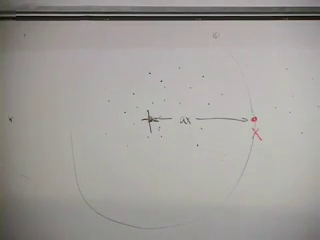
\includegraphics[width=0.70\textwidth]{lecture_08_figure_14.png}
\caption{均匀星系分布、位于共动标记 \(x\) 处的测试星系，以及其径向运动仅由所包围质量控制的球面。}
\lectureframe{01:50:05}
\end{figure}

\begin{figure}[H]
\centering
\begin{tikzpicture}[scale=0.94,>=Latex]
  \draw[gray!65] (0,0) circle (2.35);
  \foreach \p in {
    (-1.5,0.8),(-1.2,-0.8),(-0.8,1.5),(-0.6,0.35),(-0.3,-1.45),
    (0.15,1.05),(0.35,-0.55),(0.7,1.65),(0.9,0.45),(1.25,-0.9),
    (1.65,0.95),(-1.75,-0.2),(1.8,-0.15)} {
    \fill[black!55] \p circle (1.15pt);
  }
  \fill[blue!65!black] (0,0) circle (2pt)
    node[below left] {chosen origin};
  \fill[red!70!black] (2.35,0) circle (2.2pt)
    node[right] {test galaxy};
  \draw[->,thick] (0,0) -- (2.32,0)
    node[midway,above] {\(R=a(t)x\)};
  \draw[<->] (-2.35,-2.55) -- (2.35,-2.55)
    node[midway,below=4pt] {only the enclosed mass contributes};
\end{tikzpicture}
\caption{对壳层定理设置的清晰重建。原点是方便的选择，而不是宇宙的中心。}
\end{figure}

因此，宇宙学多体问题已经变成了一个熟悉的一体问题：一个抛射体在它当前球面内所包含质量的吸引下沿径向运动。牛顿方程将决定\(R=a x\)、从而\(a(t)\)如何加速。讲座有意在完成该计算之前停下。下一次会议将推导最简单的物质主导宇宙学，而不是把答案偷偷塞进几何设定中。

\section{迟来的问题：光、大爆炸与曲率}

正式讲座已经结束，但最后的问题揭示了几幅误导性的图像，它们是物理内容的一部分，而不是附录。

\begin{classroomqa}
\audiencequestion{如果来自极遥远天体的光是在宇宙小得多的时候发出的，为什么它现在看起来来自如此遥远的地方？而如果早期宇宙是致密的，为什么它并非全部可观测？}
\lecturerresponse{必须在膨胀坐标中求解零测地线方程。当\(a(t)\)非常小时，\(dx/dt=1/a(t)\)非常大：光在局域仍以\(c=1\)运动的同时，跨越了很大的共动间隔。随着\(a(t)\)增大，它的共动坐标速度减小。精确的发射点和可观测区域的大小取决于\(a(t)\)的整个历史，因此数值答案要等到某个具体宇宙学被求解之后才能给出。}
\end{classroomqa}

\begin{figure}[H]
\centering
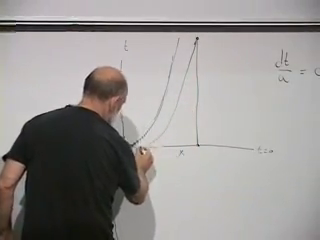
\includegraphics[width=0.72\textwidth]{lecture_08_figure_15.png}
\caption{\((x,t)\)平面中的一条光线：当\(a(t)\)很小时，在共动坐标中近乎水平，随后随着尺度因子增大而逐渐变陡。}
\lectureframe{01:56:20}
\end{figure}

对\eqref{eq:null-ray}积分使被推迟的计算变得明确：
\begin{equation}
  \Delta x
  =\int_{t_{\mathrm e}}^{t_0}\frac{dt}{a(t)}.
  \label{eq:comoving-light-distance}
\end{equation}
当\(t_{\mathrm e}\)趋近于开端时，该积分是否达到任意大的共动距离，取决于\(a(t)\)在早期时间的形式。\editorialnote{方程\eqref{eq:comoving-light-distance}是黑板方程\(dx=dt/a(t)\)的积分形式。它明确给出了讲座留给下一次会议、且尚未选择特定尺度因子的计算。}

\begin{figure}[H]
\centering
\begin{tikzpicture}[scale=0.92,>=Latex]
  \draw[->] (0,0) -- (6.4,0) node[right] {\(x\)};
  \draw[->] (0,0) -- (0,4.6) node[above] {\(t\)};
  \draw[thick,blue!65!black]
    plot[smooth] coordinates {(0,0.18) (1.65,0.42) (2.65,1.05)
      (3.35,2.05) (3.85,3.25) (4.05,4.25)};
  \fill[red!70!black] (4.05,4.25) circle (2pt)
    node[right] {reception today};
  \draw[dashed] (4.05,0) -- (4.05,4.25);
  \node[align=left] at (1.65,3.25)
    {\(\displaystyle \frac{dx}{dt}=\frac1{a(t)}\)\\
     large when \(a\) is small};
\end{tikzpicture}
\caption{共动坐标中光线构造的清晰版本。斜率的改变是坐标效应，而不是局域光速的改变。}
\end{figure}

\begin{classroomqa}
\audiencequestion{大爆炸是否从一个点抛射出物质，因此它现在应当位于一个膨胀的壳层或环上？}
\lecturerresponse{不。该模型始于一个均匀且极其致密的空间。每一个大尺度间隔都在增长；物质并不是从一个优先中心穿过预先存在的空虚空间被发射出去的。均匀布满圆点的气球是一个有用的二维类比：当它膨胀时，所有圆点间隔都增大，而表面仍保持均匀布点。空间甚至在每一个正时刻都可能是无限的；膨胀并不意味着它起初是某个别的东西内部的一个有限球。}
\end{classroomqa}

\begin{classroomqa}
\audiencequestion{在膨胀期间，引力本身是更弱还是更强？}
\lecturerresponse{讨论保持牛顿常数\(G\)固定。尽管如此，力仍会变化，因为间隔和所包含的密度会变化。更早时，同一个共动星系在物理上更近，均匀物质也更致密，因此引力减速更大。这正是壳层定理计算所要量化的内容。}
\end{classroomqa}

最后，空间曲率不可与膨胀相混淆。地球的一小块区域看起来是平的，因为其尺寸与地球半径相比极小。通过测量足够大的三角形，人们要么能探测到角盈余，要么能给出曲率半径的下界。天文学用巨大的三角形做类似的实验。在2006年讲座所用的观测语言中，在可见区域内没有探测到曲率，因此任何曲率半径都必须显著大于该区域。这并不证明宇宙恰好平坦；它限定了可及部分能有多弯曲。

对于球面，内禀曲率按\(R^{-2}\)标度。因此，一个膨胀的球面在局域上变得更平。同样，如果一个均匀宇宙具有非零空间曲率，膨胀会增大其曲率半径，并减小任何固定大小局域斑块中可见的曲率。
\editorialnote{\(R^{-2}\)标度是讲座中“数值曲率随着球面增大而减小”这一陈述的标准定量形式。}

\begin{classroomqa}
\audiencequestion{如果空间是弯曲的，宇宙是否必须有一部分在收缩而另一部分在膨胀？}
\lecturerresponse{不。正、零或负的空间曲率描述的是每一个宇宙时间切片上的几何。膨胀或收缩由\(a(t)\)的演化控制。一个弯曲的宇宙可以膨胀；一个平坦的宇宙可以收缩。膨胀之后可能逆转，正如向上运动的抛射体可能落回，但同时发生的收缩并不隐藏在曲率之中。动力学问题在于，向外的运动究竟是逃脱了所包围质量的吸引、落回，还是恰好位于临界边界上。}
\end{classroomqa}

那个逃逸速度的比较是本讲最后一个板书层面的想法。几何已经提供了度规、哈勃定律和光线方程。牛顿定理已经把动力学归结为一个球体内的质量。下一讲恰好从本讲应当结束的地方开始：从决定\(a(t)\)的方程开始，并从膨胀究竟是逃脱、再坍缩，还是恰好处于刀刃边缘这一问题开始。

\chapter{弗里德曼动力学：物质、辐射与真空能}

\lectureoverview{膨胀宇宙的运动学可以用一句话表述：物理间距随标度因子\(a(t)\)增长。现在的问题是要确定这个函数。我们将从牛顿能量守恒重新导出平直空间的弗里德曼方程，先对普通物质求解，然后看看为什么辐射和真空能会导致完全不同的宇宙历史。}

\section{待解释的几何}

在固定的宇宙时刻，大尺度宇宙看起来是均匀且各向同性的。星系、星系团和超星系团当然是真实的结构，但在数亿或数十亿光年的尺度上，它们的分布变得非常均匀。这一经验规律被称为宇宙学原理。这个名称并不能使它成为一条定理；该原理的力量来自观测。

还有第二个经验事实。在目前的精度范围内，大的空间三角形表现得如同欧几里得三角形。与测量足球场的类比是有用的。如果拉紧的线构成的三角形的内角和为\(180^\circ\)，这并没有证明地球整体上是平的。它表明的是地球的曲率半径远大于足球场。宇宙测量具有相同的逻辑形式：空间可能具有非常大的曲率半径，但在可观测区域内，它可以很好地近似为平直的。

参考几何是闵可夫斯基时空，
\begin{equation}
  d\tau^2=dt^2-\left(dx^2+dy^2+dz^2\right).
  \label{eq:l09-minkowski}
\end{equation}
括号内就是三维的欧几里得距离元。相比之下，在广义相对论中，坐标微分的系数是场。它们可以随位置和时间变化，也可能出现混合项。这些度规系数是牛顿引力场的相对论后继者。

\begin{figure}[H]
  \centering
  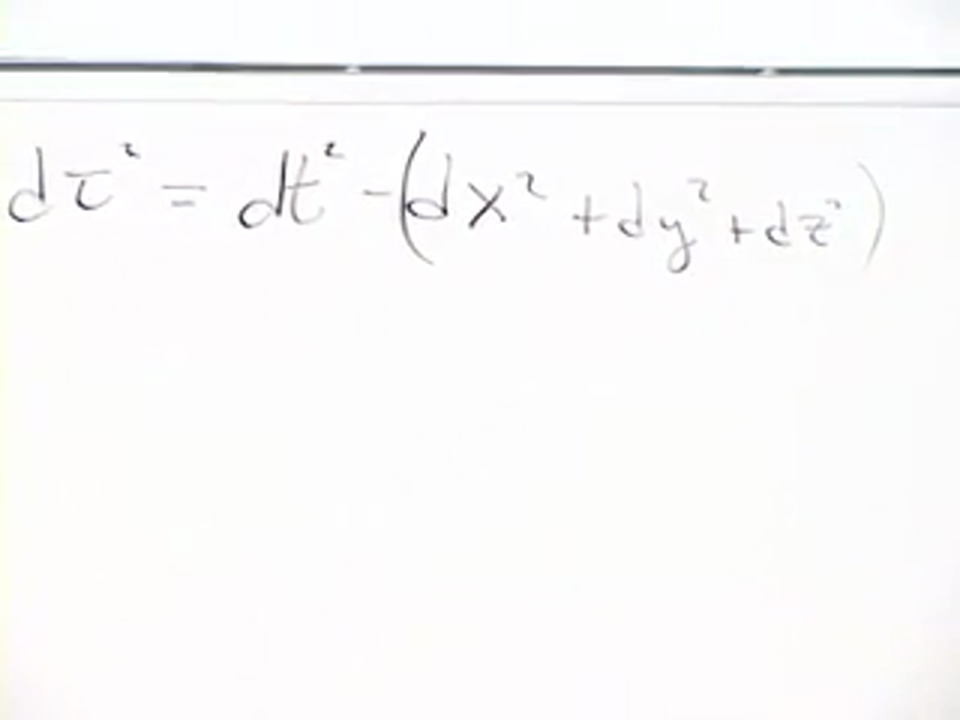
\includegraphics[width=0.72\textwidth]{lecture_09_figure_01.png}
  \caption{讲座开头写出的闵可夫斯基固有时元。源帧位于00:01:50。}
  \label{fig:l09-minkowski-board}
\end{figure}

对于空间平直的膨胀宇宙，均匀性和各向同性只留下一个依赖于时间的标度因子：
\begin{equation}
  d\tau^2=dt^2-a^2(t)\left(dx^2+dy^2+dz^2\right).
  \label{eq:l09-flat-frw}
\end{equation}
我们采用\(c=1\)的单位制，因此时间和长度具有相同的量纲。有两种自洽的约定。可以赋予\(x,y,z\)长度的量纲并取\(a\)无量纲，或者把\(x,y,z\)视为无量纲的标签而让\(a\)带有长度的量纲。本讲座采用第二种约定，因为它使\(a(t)\)的物理意义变得可见。

\begin{figure}[H]
  \centering
  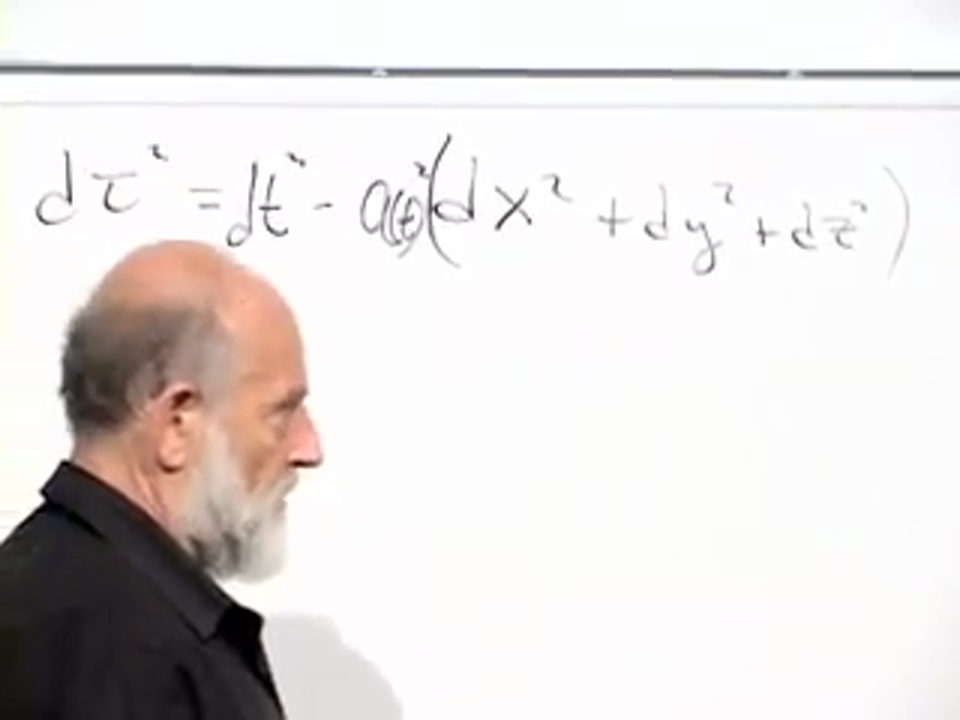
\includegraphics[width=0.72\textwidth]{lecture_09_figure_02.png}
  \caption{平直膨胀度规，其中标度因子乘以欧几里得空间线元。源帧位于00:09:12。}
  \label{fig:l09-expanding-metric-board}
\end{figure}

想象坐标被画在一块橡胶片上。坐标标记始终附着在橡胶片上，而它们之间的物理距离却在增长。因此，诸如“从\(x=0\)到\(x=1\)”这样的坐标差只是一对标签。该间隔所代表的距离是\(a(t)\)。找出支配这个标度因子的方程，就是本讲座的动力学问题。

\section{闭合、平直与开放的空间几何}

平直性是一种观测上的简化，而不是均匀性的结果。存在三种均匀且各向同性的空间几何：正曲率、零曲率和负曲率。要理解正曲率的情形，有必要对维数保持精确。

轨迹
\begin{equation}
  X_1^2+X_2^2=R^2
\end{equation}
是一个圆，即一维球面\(S^1\)。它填充的内部是一个圆盘，也称为二维球。增加一个嵌入坐标得到
\begin{equation}
  X_1^2+X_2^2+X_3^2=R^2,
\end{equation}
普通的二维球面\(S^2\)。再增加第四个嵌入坐标得到
\begin{equation}
  X_1^2+X_2^2+X_3^2+X_4^2=R^2,
  \label{eq:l09-three-sphere}
\end{equation}
三维球面\(S^3\)，它本身就是一个三维空间。我们无法想象它的四维嵌入，但内禀几何并不需要那个嵌入才能存在。

\begin{figure}[H]
  \centering
  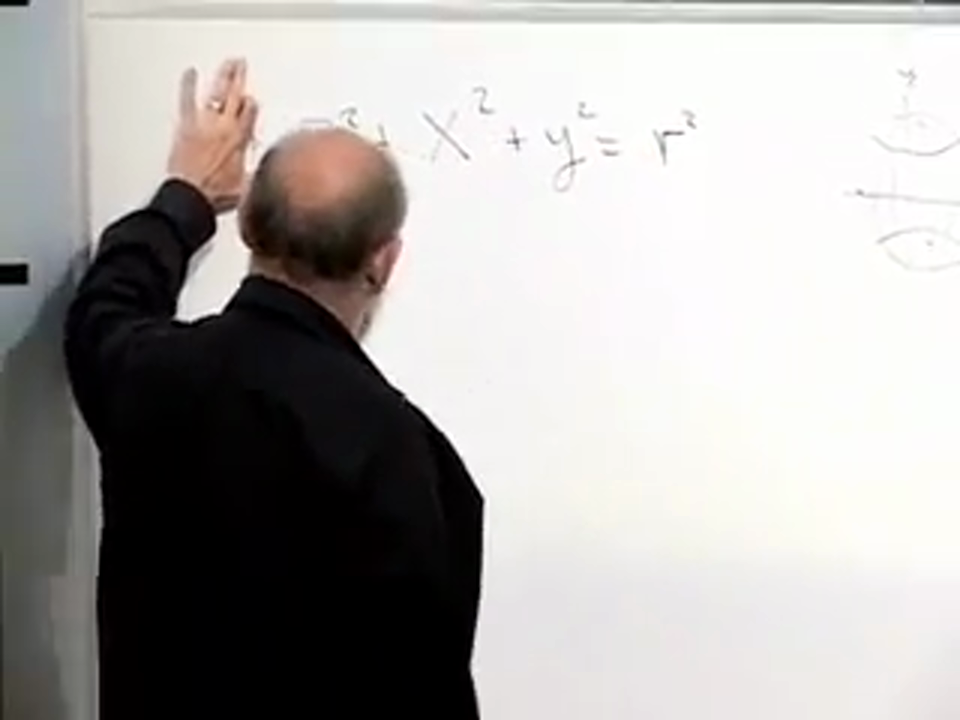
\includegraphics[width=0.72\textwidth]{lecture_09_figure_03.png}
  \caption{用于引入三维球面的嵌入方程。源帧位于00:16:40。}
  \label{fig:l09-three-sphere-board}
\end{figure}

理想球面上的每一点在几何上都与其他任何一点等价，一点处的每个方向也都等价。因此球面既是均匀的又是各向同性的。如果它的半径乘以\(a(t)\)，整个空间就会膨胀或收缩，而不会在球面上选出一个中心。将这样的宇宙回溯过去，并不会把所有物质都置于外部虚空中的一个特殊位置。整个空间都变小了，因此每一对点都彼此靠近。大爆炸并不是从空间中的某一点发生的爆炸。

在正曲率的球面上，测地三角形的内角和大于
\(180^\circ\)。平坦三角形的内角和恰好为 \(180^\circ\)。在由马鞍面不完美地代表的均匀负曲率几何中，内角和小于 \(180^\circ\)。这些内禀检验区分了这三种情形。

\begin{figure}[H]
  \centering
  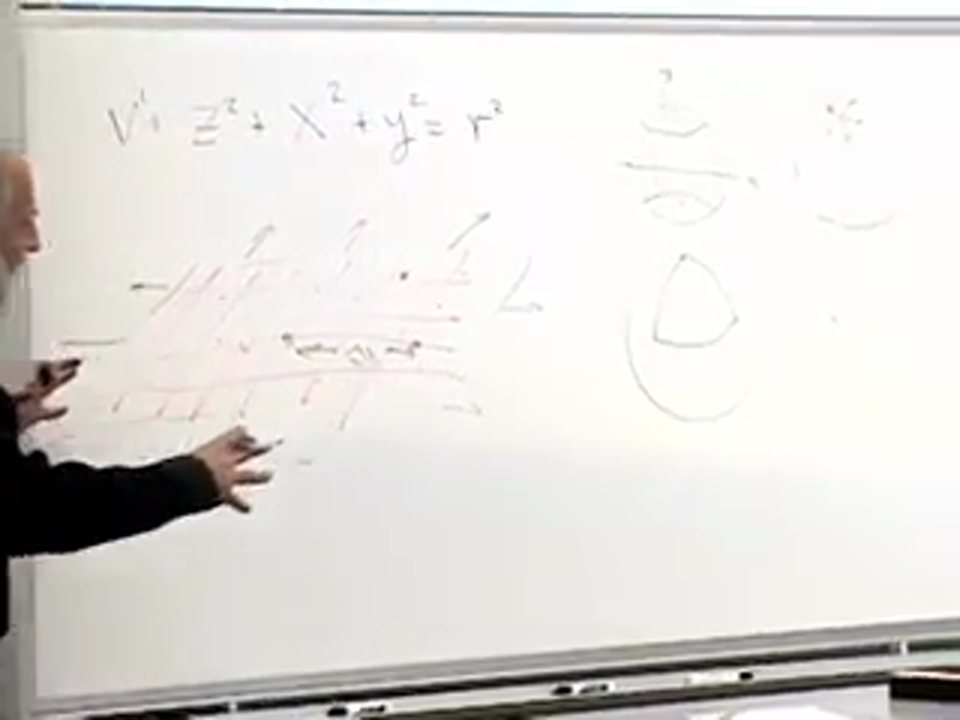
\includegraphics[width=0.72\textwidth]{lecture_09_figure_07.png}
  \caption{通过其特征三角形形状勾勒出的正、零与负曲率。源帧位于 00:37:30。}
  \label{fig:l09-curvature-board}
\end{figure}

一个完全平坦的局部度规本身并不能证明空间在拓扑上是无限的。紧致平坦拓扑在数学上是可能的，尽管本讲采用最简单的无限欧几里得模型。
\editorialnote{这一整体拓扑上的限定条件对于后续任何局部动力学都不需要。}

\section{共动标签与哈勃定律}

现在回到膨胀的平坦薄片，并在其上画一个坐标网格。在共动坐标中，网格随大尺度物质流一起膨胀。一个星系，或者更准确地说，一个足够粗粒化的星系团，保持近似固定的坐标标签，尽管它与另一个共动物体的物理距离在变化。

\begin{figure}[H]
  \centering
  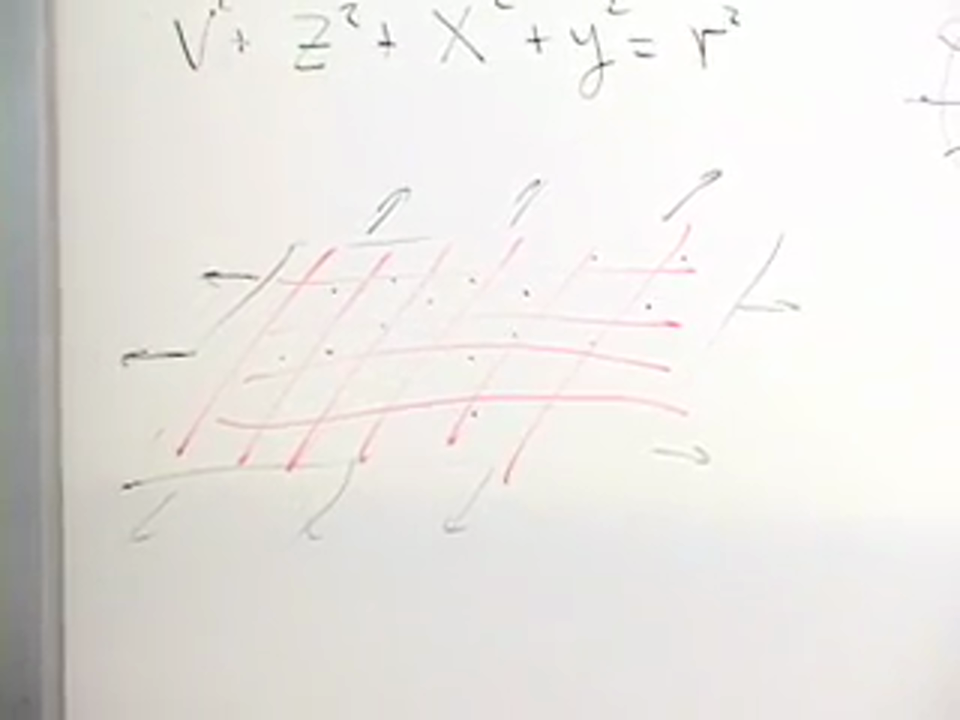
\includegraphics[width=0.72\textwidth]{lecture_09_figure_04.png}
  \caption{随膨胀空间薄片一起被携带的坐标网格。
  源帧位于 00:22:20。}
  \label{fig:l09-comoving-grid-board}
\end{figure}

对于沿 \(x\) 轴以固定共动间隔 \(\Delta x\) 分隔的两个物体，它们的物理距离为
\begin{equation}
  D(t)=a(t)\,\Delta x.
  \label{eq:l09-physical-distance}
\end{equation}
在保持 \(\Delta x\) 固定的情况下求导，得到
\begin{equation}
  v(t)=\dot a(t)\,\Delta x
      =\frac{\dot a(t)}{a(t)}D(t).
\end{equation}
定义
\begin{equation}
  H(t)\equiv\frac{\dot a(t)}{a(t)},
  \label{eq:l09-hubble-parameter}
\end{equation}
我们得到哈勃定律，
\begin{equation}
  v=H(t)D.
  \label{eq:l09-hubble-law}
\end{equation}
“哈勃常数”中的“常数”一词意味着在指定的宇宙时刻在空间各处为常数。它并不意味着在整个宇宙历史中恒定不变。

\begin{figure}[H]
  \centering
  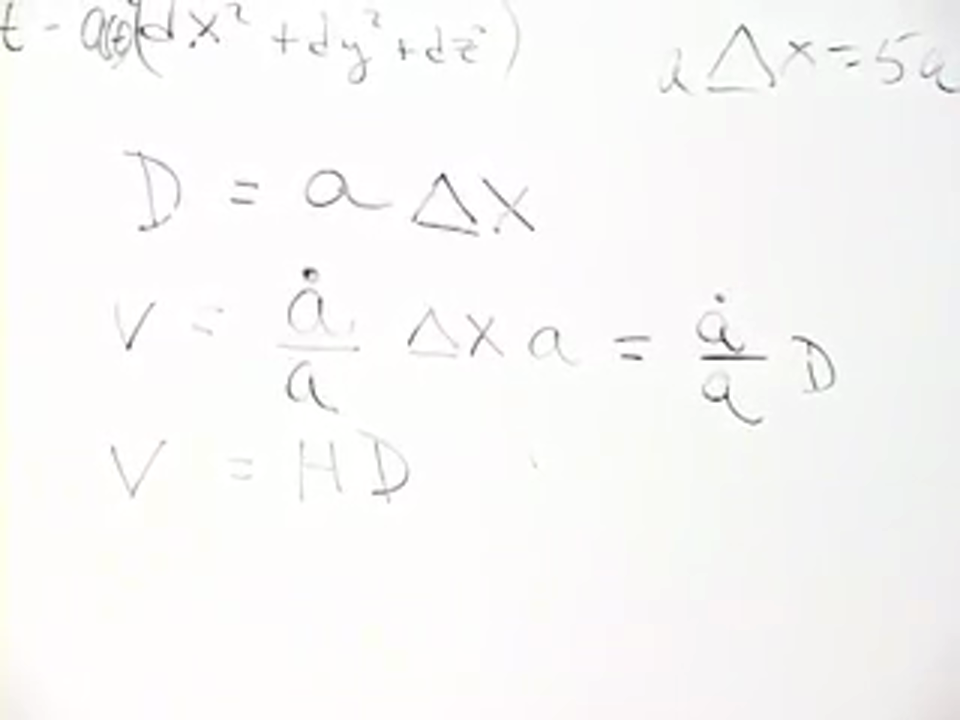
\includegraphics[width=0.72\textwidth]{lecture_09_figure_05.png}
  \caption{黑板推导 \(D=a\Delta x\)，
  \(v=(\dot a/a)D=HD\)。源帧位于 00:26:40。}
  \label{fig:l09-hubble-board}
\end{figure}

\begin{classroomqa}
\audiencequestion{如果一个遥远星系是在更早的时刻被看到的，那么推断出的哈勃参数真的应该等于今天在附近测得的值吗？}
\lecturerresponse{只有当回溯时间与宇宙年龄相比很小时才是如此。在中等距离上，\(H(t)\) 变化足够小，以至于一个数值仍然有用。在真正宇宙学尺度上，我们看到的是更早的时期，因此必须计入 \(a\) 和 \(H\) 的时间依赖性。这就是我们需要关于标度因子的动力学方程的原因之一。}
\end{classroomqa}

\section{膨胀坐标系中的零测地线}

\begin{classroomqa}
\audiencequestion{标度因子会影响光在遥远星系之间的传播吗？}
\lecturerresponse{光线沿零测地线传播，因此 \(d\tau=0\)。对于沿正 \(x\) 轴运动的光线，\(dy=dz=0\)，而膨胀的度规给出
\begin{align}
  0&=dt^2-a^2(t)dx^2,
  &dt&=a(t)dx,\notag\\
  &&\frac{dx}{dt}&=\frac{1}{a(t)}.
  \label{eq:l09-null-ray}
\end{align}
坐标速度随着 \(a(t)\) 增大而减小，但光的局部物理速度仍为 \(c=1\)。固定的坐标间隔代表不断增大的物理距离。}
\end{classroomqa}

\begin{figure}[H]
  \centering
  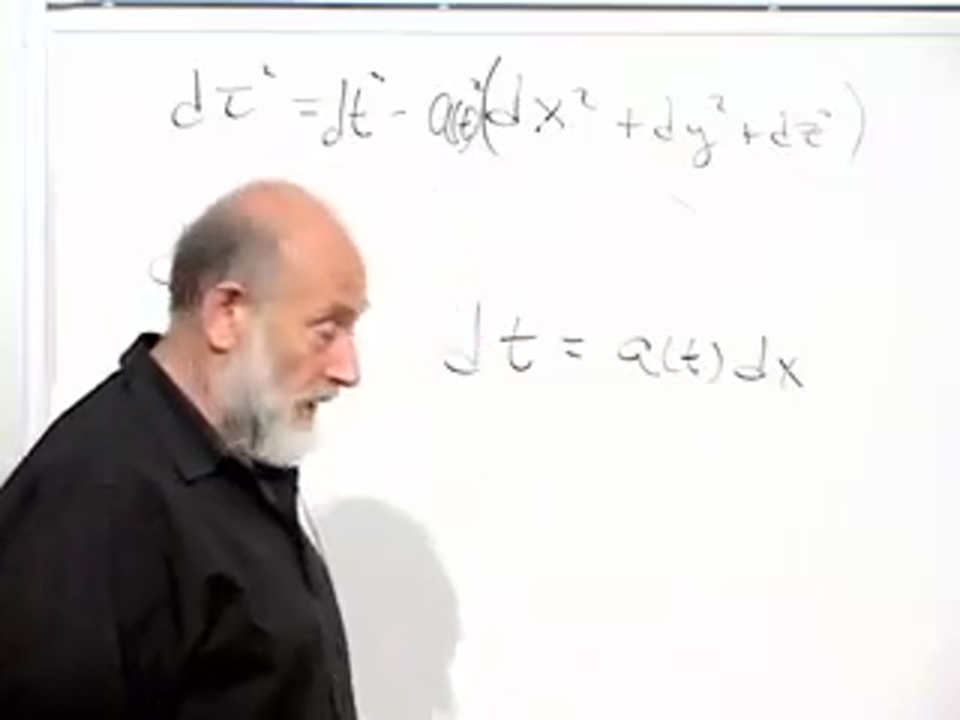
\includegraphics[width=0.72\textwidth]{lecture_09_figure_06.png}
  \caption{零条件与径向光传播的 \(dt=a(t)dx\)。
  源帧位于 00:30:54。}
  \label{fig:l09-null-board}
\end{figure}

人们可以选择这样的坐标，使得同一事实听起来像是“光在更远处变慢”，但这样一来，长度和时钟就会获得相应别扭的描述。膨胀空间的语言更简洁，因为它保留了局部陈述：每个自由下落的观测者测得相同的光速。

\begin{classroomqa}
\audiencequestion{有证据表明遥远星系中的局部光传播和原子物理是相同的吗？}
\lecturerresponse{只有无量纲比较在操作上才有意义。选择原子尺度作为长度单位，选择原子或核周期作为时间单位，然后问光穿过所选长度需要多少个这样的周期。光谱观测支持这样的陈述：这些无量纲比值在遥远区域是相同的。证据是间接的，但它恰恰是用来检验局部定律均匀性的那类比较。}
\end{classroomqa}

当可观测宇宙极其小时，光可以在相应的光穿越单位内迅速穿过给定的物理区域。这并不意味着 \(c\) 不同。它意味着该区域本身很小。

\section{宇宙内部的牛顿球}

现在我们从运动学转向动力学。把我们自己置于原点，画一个足够大的球面，使其包含许多星系和星系团。在其边界上选取一个星系。在均匀宇宙中，质量分布相对于我们呈球对称，而牛顿壳层定理给出两个关键事实：
\begin{enumerate}
  \item 所有分布在所选半径之外的球对称物质，对边界星系施加的净牛顿力为零；
  \item 球内所有物质，对于这种径向运动而言，其作用就如同全部集中在中心一样。
\end{enumerate}
我们使用一个我们处于静止的参考系，因此以下论证中的速度和加速度都是相对于我们测量的。

\begin{figure}[H]
  \centering
  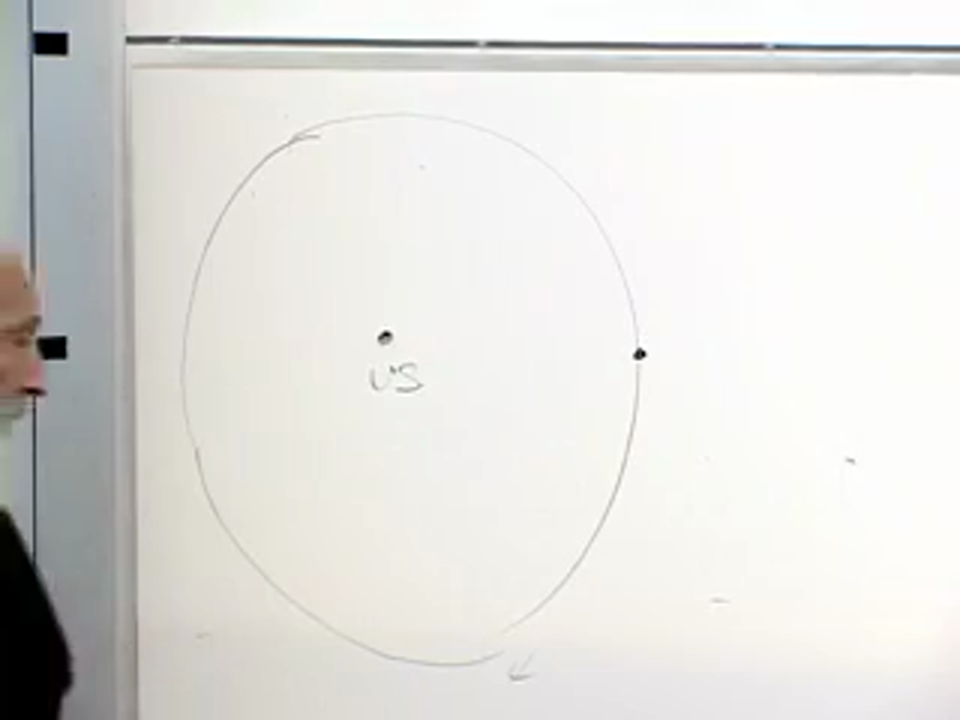
\includegraphics[width=0.72\textwidth]{lecture_09_figure_08.png}
  \caption{壳层定理的构造：我们位于中心，一个测试星系位于一个大的均匀球面的边界上。源帧位于 00:41:10。}
  \label{fig:l09-shell-board}
\end{figure}

\begin{figure}[H]
  \centering
  \begin{tikzpicture}[scale=0.92,>=Latex]
    \draw[thick] (0,0) circle (2.35);
    \fill (0,0) circle (2pt) node[below left] {us};
    \fill (2.35,0) circle (2.2pt) node[right] {test galaxy \(m\)};
    \draw[->,thick,blue!65!black] (0.18,0) -- (2.15,0)
      node[midway,above] {\(R=a(t)x\)};
    \draw[->,thick,red!65!black] (2.35,0.12) -- (3.25,0.12)
      node[midway,above] {\(v=\dot a(t)x\)};
    \node[align=center,text width=7cm] at (0,-2.85)
      {outside shells cancel;\\enclosed mass acts at the center};
  \end{tikzpicture}
  \caption{牛顿构造的清晰重建。}
  \label{fig:l09-shell-clean}
\end{figure}

如果该星系具有固定的共动坐标 \(x\)，则其物理半径和速度为
\begin{equation}
  R(t)=x a(t),
  \qquad
  v(t)=x\dot a(t)=H(t)R(t).
  \label{eq:l09-radius-velocity}
\end{equation}
设 \(M\) 为球面所包围的质量，\(m\) 为测试星系的质量。牛顿能量为
\begin{equation}
  E=\frac12 m v^2-\frac{GMm}{R}.
  \label{eq:l09-newtonian-energy}
\end{equation}

\begin{figure}[H]
  \centering
  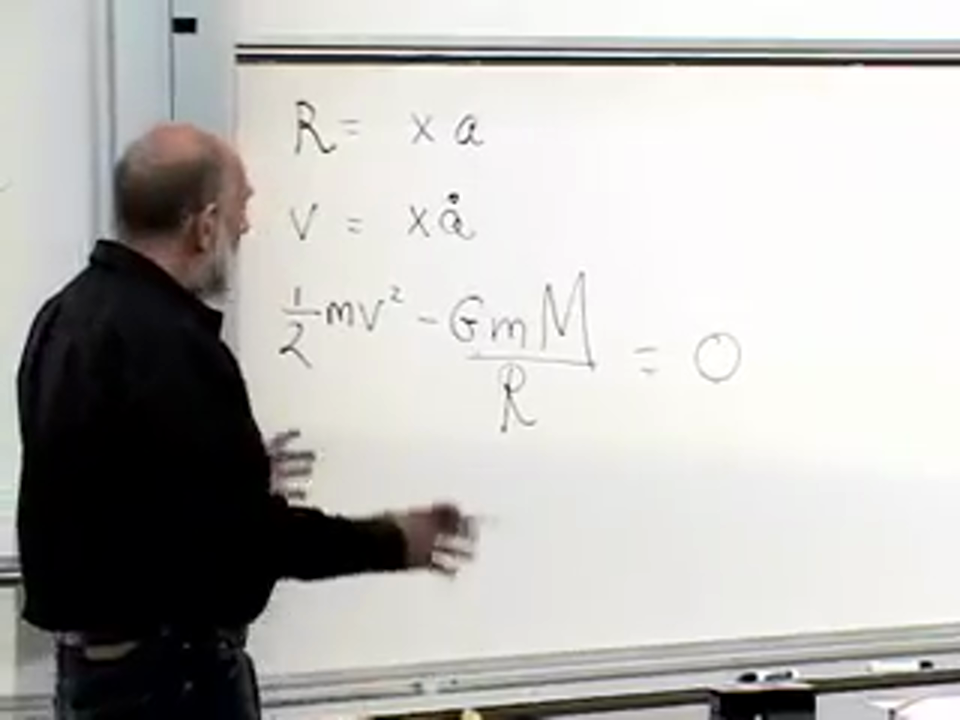
\includegraphics[width=0.72\textwidth]{lecture_09_figure_09.png}
  \caption{完整的板书序列 \(R=xa\)、\(v=x\dot a\)，以及针对 \(E=0\) 特化的牛顿能量方程。源帧位于 00:48:40。}
  \label{fig:l09-energy-board}
\end{figure}

能量可以为正、为零或为负。从逃逸与再坍缩之间的边界开始，\(E=0\)，对此有
\begin{equation}
  \frac12 v^2=\frac{GM}{R}.
  \label{eq:l09-zero-energy}
\end{equation}

\begin{classroomqa}
\audiencequestion{对于退行星系，总能量为零意味着什么？}
\lecturerresponse{这恰好就是逃逸速度的情形。正的能量意味着运动高于逃逸速度；负的能量意味着运动低于逃逸速度，并且在仅有物质的牛顿图像中，最终会返回。我们从这些可能性之间的边界开始，并在推导出平坦方程之后再回到其他符号。}
\end{classroomqa}

\begin{classroomqa}
\audiencequestion{所包围的质量 \(M\) 会随着球面膨胀而变化吗？}
\lecturerresponse{不会。该球面是共动的，因此同样的粒子始终留在其内部。它的物理体积增大，密度下降，但其总包围质量保持固定。\(M\) 与 \(\rho(t)\) 之间的这一区分至关重要。}
\end{classroomqa}

对于均匀密度 \(\rho(t)\)，
\begin{equation}
  M=\frac{4\pi}{3}\rho(t)R^3.
  \label{eq:l09-enclosed-mass}
\end{equation}
代入 \eqref{eq:l09-zero-energy} 得到
\begin{equation}
  \frac12 v^2
  =\frac{G}{R}\left(\frac{4\pi}{3}\rho R^3\right).
  \label{eq:l09-enclosed-energy}
\end{equation}

\begin{figure}[H]
  \centering
  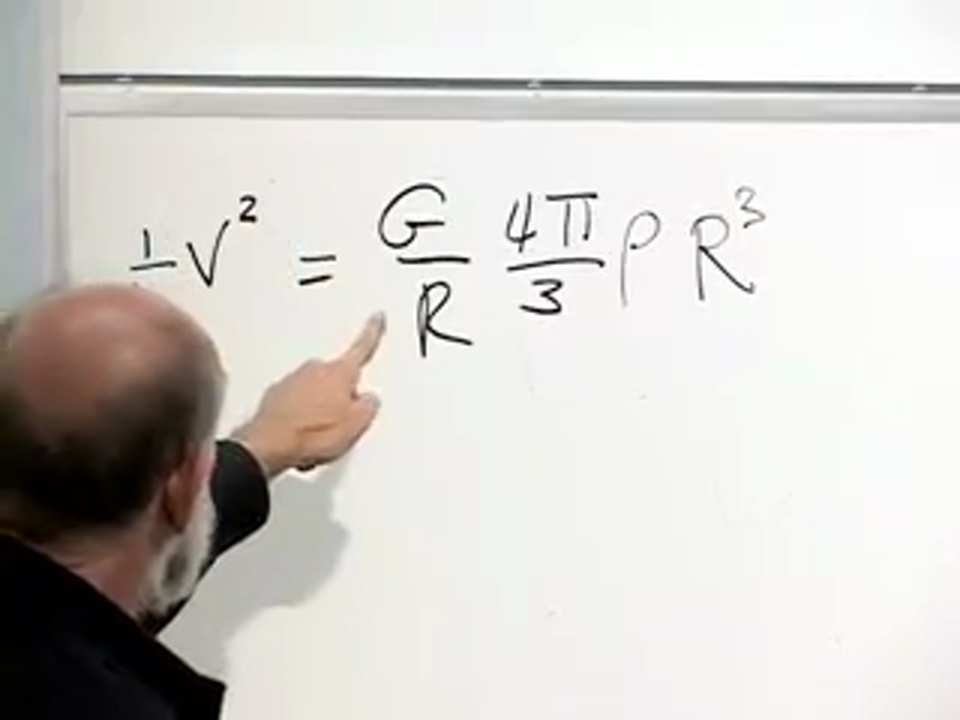
\includegraphics[width=0.72\textwidth]{lecture_09_figure_10.png}
  \caption{零能量方程中的包围质量代换。源帧位于 00:54:16.060。}
  \label{fig:l09-enclosed-mass-board}
\end{figure}

利用 \(v=HR\)，我们得到
\begin{align}
  \frac12 H^2R^2
    &=\frac{4\pi G}{3}\rho R^2,\\
  H^2
    &=\frac{8\pi G}{3}\rho.
\end{align}
因此，零能量、空间平坦的膨胀定律为
\begin{equation}
  \boxed{\left(\frac{\dot a}{a}\right)^2
  =\frac{8\pi G}{3}\rho(t)}.
  \label{eq:l09-flat-friedmann}
\end{equation}
\(R^2\) 的消去并非偶然。一个均匀宇宙无论选择哪个共动星系作为测试对象，都必须给出相同的 \(H(t)\)。

\begin{figure}[H]
  \centering
  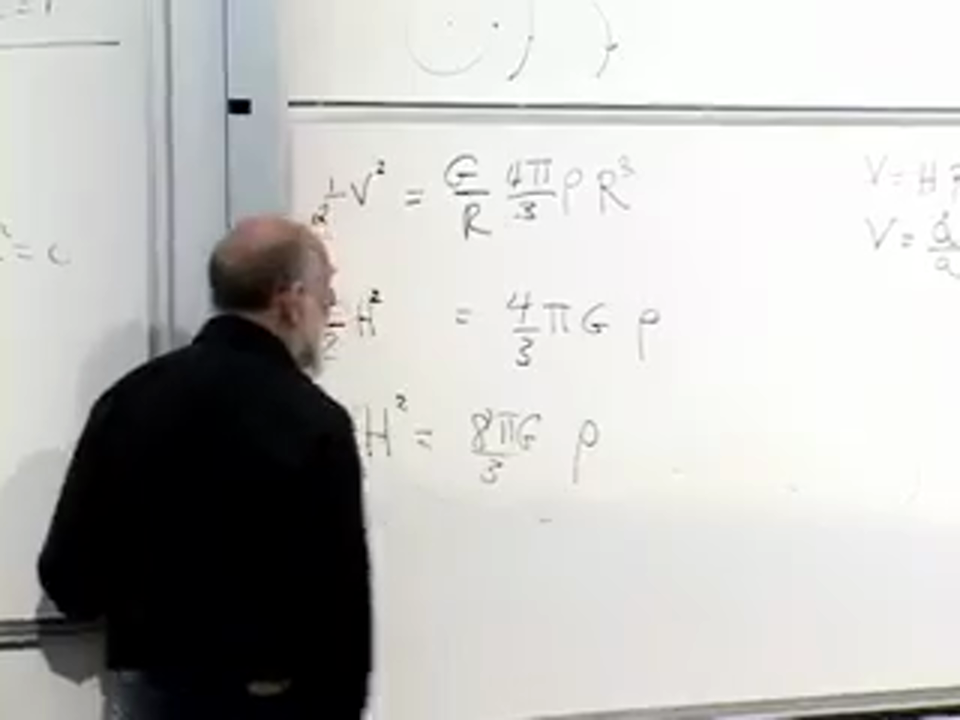
\includegraphics[width=0.72\textwidth]{lecture_09_figure_11.png}
  \caption{半径的消去以及由此得到的平坦弗里德曼关系在板书上。源帧位于 00:57:30。}
  \label{fig:l09-friedmann-board}
\end{figure}

\begin{classroomqa}
\audiencequestion{有证据支持零能量关系吗？}
\lecturerresponse{两边都可以通过观测推断：\(H\) 来自退行数据，而 \(\rho\) 则通过计入恒星、气体、暗物质和真空能量得到。讲座时代的比较发现两边在约百分之几的精度内一致。这一限定很重要：必须包括所有形式的能量，而后面对真空能量的讨论会改变朴素的逃逸速度解释。}
\end{classroomqa}

在单位 \(c=1\) 下，质量密度和能量密度具有相同的单位。因此符号 \(\rho\) 将表示适用于所讨论组分的总能量密度。

\section{普通物质与三分之二定律}

方程 \eqref{eq:l09-flat-friedmann} 在知道 \(\rho(t)\) 如何变化之前并不封闭。首先用一个缓慢运动的非相对论性粒子填充一个共动长方体盒子。它的坐标尺寸固定，而其物理体积按如下方式增长：
\begin{equation}
  V(t)=a^3(t)\,\Delta x\,\Delta y\,\Delta z.
\end{equation}
盒子中的粒子数和静质量保持固定，因此
\begin{equation}
  \rho_{\mathrm m}(t)=\frac{C_{\mathrm m}}{a^3(t)}.
  \label{eq:l09-matter-dilution}
\end{equation}
归一化到当前时期 \(t_0\)，
\begin{equation}
  \frac{\rho_{\mathrm m}(t)}{\rho_{\mathrm m,0}}
  =\left(\frac{a_0}{a(t)}\right)^3.
  \label{eq:l09-matter-normalized}
\end{equation}

\begin{figure}[H]
  \centering
  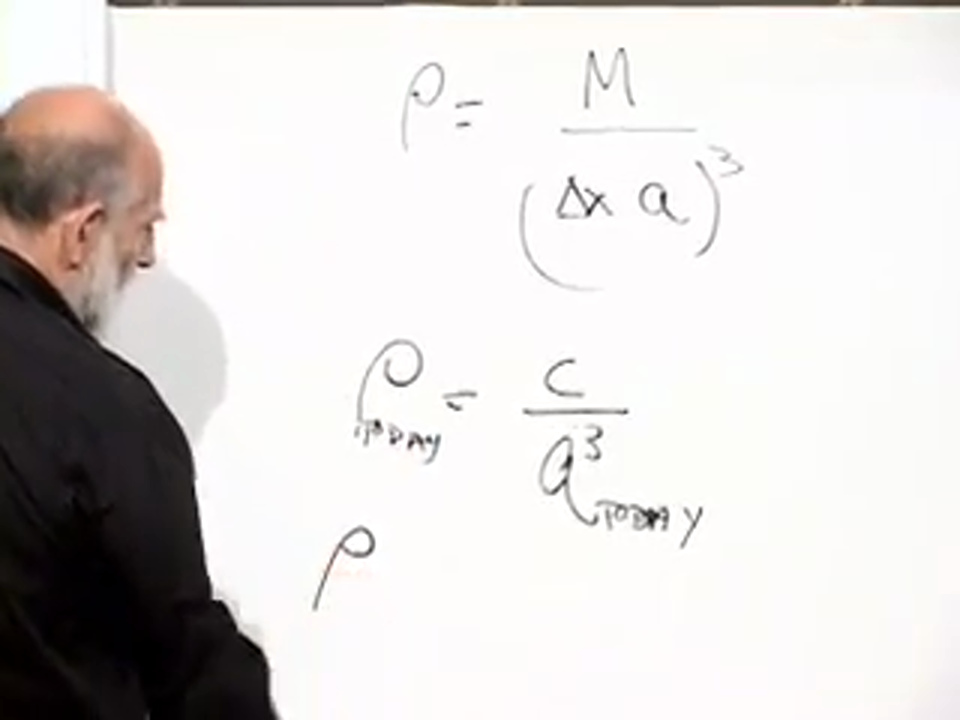
\includegraphics[width=0.72\textwidth]{lecture_09_figure_12.png}
  \caption{物质密度、其 \(a^{-3}\) 稀释以及当今归一化。源帧位于 01:04:47.940。}
  \label{fig:l09-density-board}
\end{figure}

\begin{classroomqa}
\audiencequestion{目前宇宙的能量密度大致是多少，仅靠普通原子能提供吗？}
\lecturerresponse{对可见重子物质的计数只给出了答案的一部分。暗物质和暗能量也必须以等效质能的形式计入。讲座引用了一个粗略的尺度范围，从每立方米一个原子到几十个氢质量当量，强调的是数量级而非精确清单。}
\end{classroomqa}

将\eqref{eq:l09-matter-dilution}代入\eqref{eq:l09-flat-friedmann}，并把所有与时间无关的因子吸收进一个正常数\(C\)：
\begin{equation}
  \left(\frac{\dot a}{a}\right)^2=\frac{C}{a^3},
  \qquad
  \dot a^2=\frac{C}{a}.
  \label{eq:l09-matter-ode}
\end{equation}
有两种直截了当的方法可以求解它。幂律试探解\(a=K t^p\)要求
\begin{equation}
  p-1=-\frac{p}{2},
  \qquad p=\frac23.
\end{equation}
等价地，取膨胀的平方根分支并积分：
\begin{equation}
  a^{1/2}\frac{da}{dt}=\sqrt C,
  \qquad
  \int a^{1/2}da=\sqrt C\int dt,
\end{equation}
因此，在选定大爆炸作为时间原点之后，
\begin{equation}
  a^{3/2}\propto t,
  \qquad
  \boxed{a(t)\propto t^{2/3}}.
  \label{eq:l09-matter-solution}
\end{equation}
现场推导在匹配系数时短暂丢失了一个因子，随后回到积分并验证了指数。笔记保留了这一检验，但只展示修正后的代数运算。

\begin{figure}[H]
  \centering
  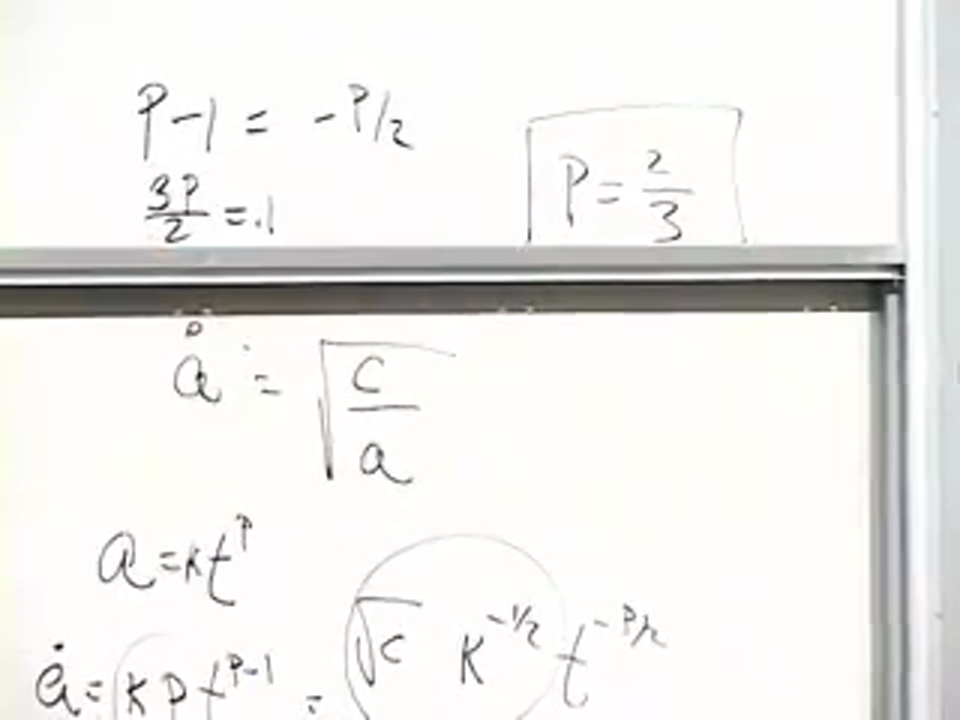
\includegraphics[width=0.72\textwidth]{lecture_09_figure_13.png}
  \caption{幂律试探解与加框的指数\(p=2/3\)。源帧位于01：13：05。}
  \label{fig:l09-matter-solution-board}
\end{figure}

对解求导得到
\begin{equation}
  H(t)=\frac{\dot a}{a}=\frac{2}{3t}.
  \label{eq:l09-matter-hubble}
\end{equation}
哈勃参数在过去更大。因此，当看得足够远以观察到可观的回溯时间时，不应使用今天的\(H_0\)不变来外推局域线性关系。

\begin{figure}[H]
  \centering
  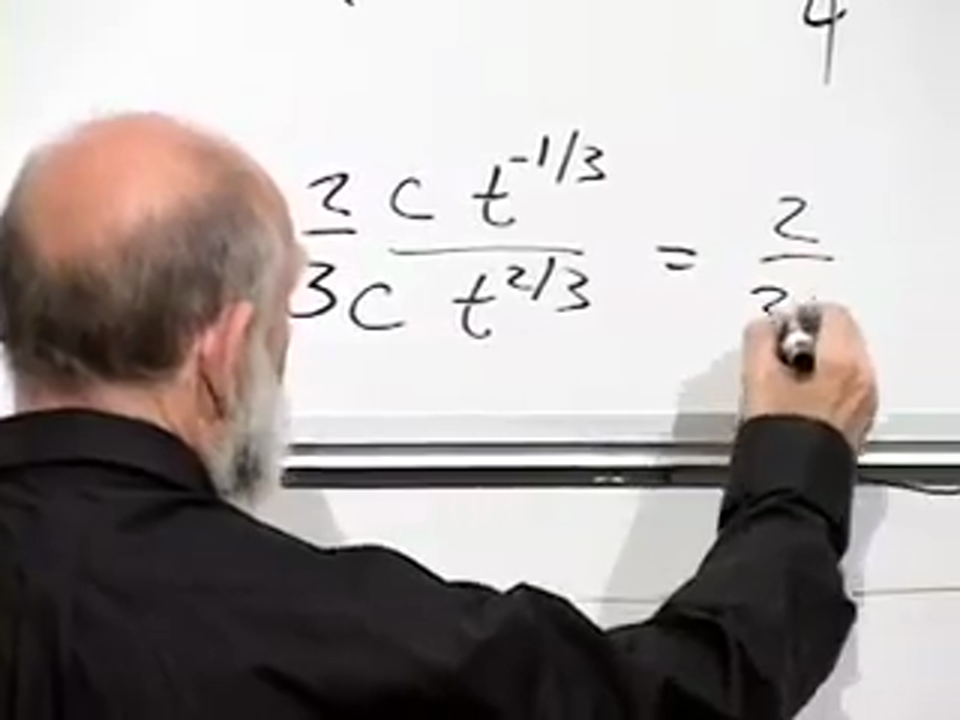
\includegraphics[width=0.72\textwidth]{lecture_09_figure_14.png}
  \caption{取\(\dot a/a\)对于\(a\propto t^{2/3}\)得到
  \(H=2/(3t)\)。源帧位于01：20：42。}
  \label{fig:l09-hubble-time-board}
\end{figure}

\section{能量符号与空间曲率}

牛顿式的推理已经带领我们走过了平坦的零能量情形。广义相对论补充了一个仅靠壳层定理无法得到的事实：牛顿式比能量的符号对应于空间曲率的符号。
\begin{center}
\begin{tabular}{@{}>{\raggedright\arraybackslash}p{0.20\linewidth}
                    >{\raggedright\arraybackslash}p{0.29\linewidth}
                    >{\raggedright\arraybackslash}p{0.37\linewidth}@{}}
  \toprule
  总能量 & 空间曲率 & 仅含物质时的命运 \\
  \midrule
  正 & 负（开放） & 永远膨胀 \\
  零 & 零（平坦） & 趋近逃逸边界 \\
  负 & 正（闭合） & 膨胀、反转、再坍缩 \\
  \bottomrule
\end{tabular}
\end{center}
最后一列假设没有真空能。在抛射体类比中，正能量意味着高于逃逸速度，零意味着恰好等于逃逸速度，负意味着低于逃逸速度。爱因斯坦方程将这三种情形分别与开放、平坦和闭合的空间几何对应起来。

\section{光子与二分之一定律}

物质定律 \(\rho\propto a^{-3}\) 假设每个粒子的能量近似固定，而数密度下降。光子违反这一假设。对于光子，
\begin{equation}
  E=h\nu=\frac{hc}{\lambda}.
\end{equation}
膨胀使其波长与尺度因子成正比地拉伸，
\begin{equation}
  \lambda\propto a,
  \qquad E\propto a^{-1}.
\end{equation}
光子数密度仍按 \(a^{-3}\) 下降，而每个光子的能量又贡献一个额外的 \(a^{-1}\) 因子。因此
\begin{equation}
  \boxed{\rho_{\mathrm r}(t)\propto a^{-4}(t)}.
  \label{eq:l09-radiation-dilution}
\end{equation}

吉他弦类比抓住了物理图像。拨动一根弦，然后拉长其振动部分：波长变长，音调降低。膨胀共动盒中的光子模式行为类似。将这一图像反向运行，压缩会缩短波长并提高光子能量。

\begin{figure}[H]
  \centering
  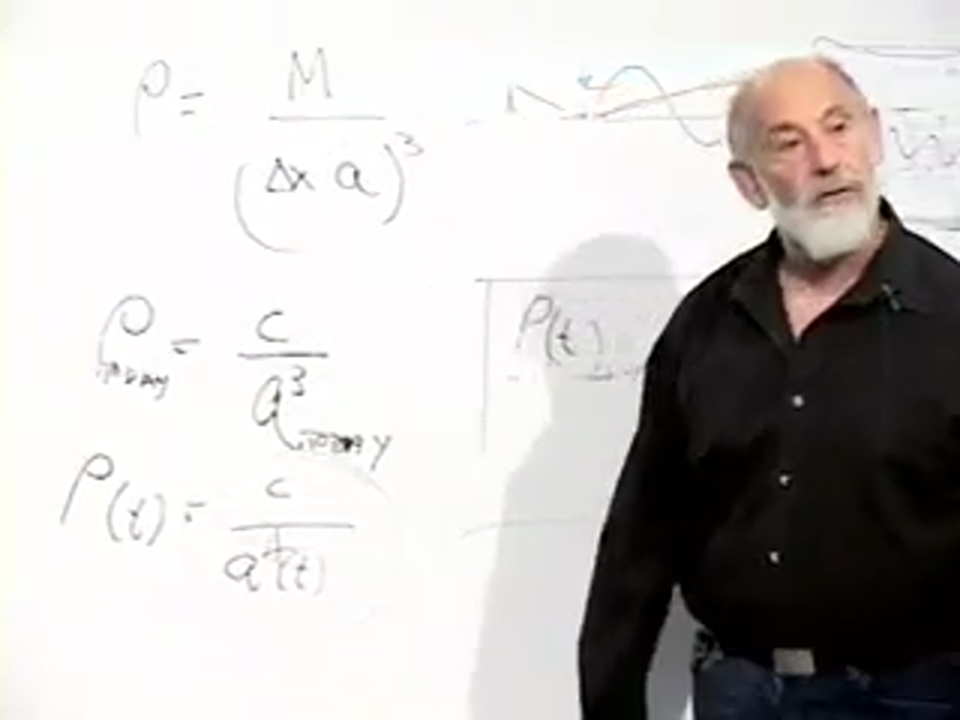
\includegraphics[width=0.72\textwidth]{lecture_09_figure_15.png}
  \caption{黑板上将物质密度关系推广到辐射标度 \(\rho_{\mathrm r}\propto a^{-4}\)。源帧在 01:29:20。}
  \label{fig:l09-radiation-board}
\end{figure}

在平坦弗里德曼方程中使用 \(\rho_{\mathrm r}\propto a^{-4}\) 得到
\begin{equation}
  \left(\frac{\dot a}{a}\right)^2=\frac{C_{\mathrm r}}{a^4},
  \qquad
  \dot a\propto a^{-1},
\end{equation}
因而
\begin{equation}
  \boxed{a(t)\propto t^{1/2}}.
  \label{eq:l09-radiation-solution}
\end{equation}
这比 \(t^{2/3}\) 增长得更慢。回溯到足够远的过去，辐射必定支配普通物质，因为当 \(a\) 减小时，\(a^{-4}\) 比 \(a^{-3}\) 上升得更快。讲座将物质-辐射交叉点置于尺度因子大约比今天小一千倍的时代附近。在该交叉点之前，宇宙由辐射支配；之后，在很长一段时期内，它由物质支配。

\section{真空能与指数膨胀}

真空能具有相反的标度行为。其密度是空无一物的空间的一种属性，并不随宇宙膨胀而稀释：
\begin{equation}
  \rho_\Lambda=\text{constant}.
  \label{eq:l09-vacuum-density}
\end{equation}
普通物质和辐射越回溯过去越致密，而这一项则不然。因此它在早期宇宙中较不重要，而随着其他组分稀释，它变得越来越重要。讲座使用当时的估计：真空能提供了今天宇宙能量密度的大约 \(70\%\)。

在\(\rho_\Lambda\)恒定的情况下，方程\eqref{eq:l09-flat-friedmann}给出恒定的膨胀率
\begin{equation}
  H_\Lambda=\sqrt{\frac{8\pi G}{3}\rho_\Lambda},
  \qquad
  \frac{\dot a}{a}=H_\Lambda.
\end{equation}
因此
\begin{equation}
  \boxed{a(t)=a(t_i)e^{H_\Lambda(t-t_i)}}.
  \label{eq:l09-vacuum-solution}
\end{equation}

\begin{figure}[H]
  \centering
  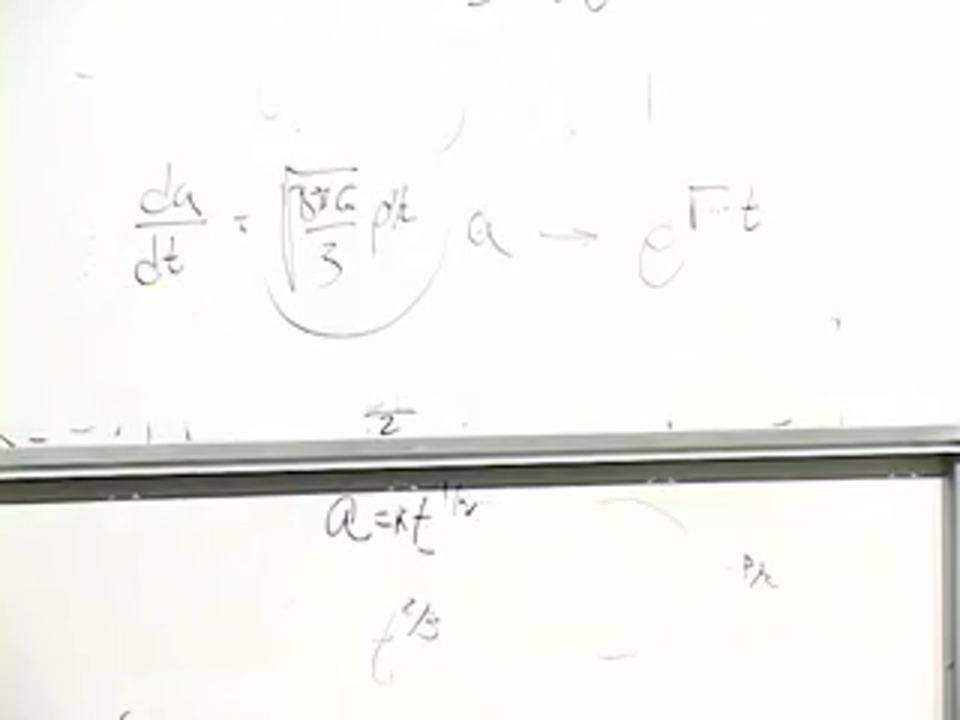
\includegraphics[width=0.72\textwidth]{lecture_09_figure_16.png}
  \caption{导致指数膨胀的常密度方程。
  源帧位于01:35:48。}
  \label{fig:l09-vacuum-board}
\end{figure}

在讲座中引用的观测尺度上，宇宙的线尺度在大约一百亿到一百二十亿年间翻倍。这一微小但非零的真空密度的起源仍未得到解释；它的存在及其对膨胀的影响是经验事实。

\begin{classroomqa}
\audiencequestion{在这一讨论中，真空能量与暗能量是同一回事吗？}
\lecturerresponse{是的。这里“暗能量”指恒定的真空能量密度，等价于宇宙学常数。可以设想更一般的随时间变化的暗能量模型，但它们不属于本讲座计算的一部分。}
\end{classroomqa}

\section{膨胀的宇宙如何使光红移}

\begin{classroomqa}
\audiencequestion{光子如何知道我们选择了膨胀的共动坐标，从而降低它们的能量？}
\lecturerresponse{它们并不对我们的标记作出响应。它们传播所经过的几何，其物理间隔在变化。占据一个物理尺寸翻倍的区域的波列，其波长也翻倍。共动坐标只是经济地描述这种拉伸；它们并不导致这种拉伸。}
\end{classroomqa}

\begin{classroomqa}
\audiencequestion{今天到达我们的背景光子来自哪里？}
\lecturerresponse{看得越远意味着看得越早。最终我们看到宇宙物质是电离等离子体的时代，由于光子被自由带电粒子反复散射，该等离子体是不透明的。光子能够最后一次自由地旅行到我们的那个边界，表现为围绕观测者的一个球面：最后散射面。}
\end{classroomqa}

\begin{figure}[H]
  \centering
  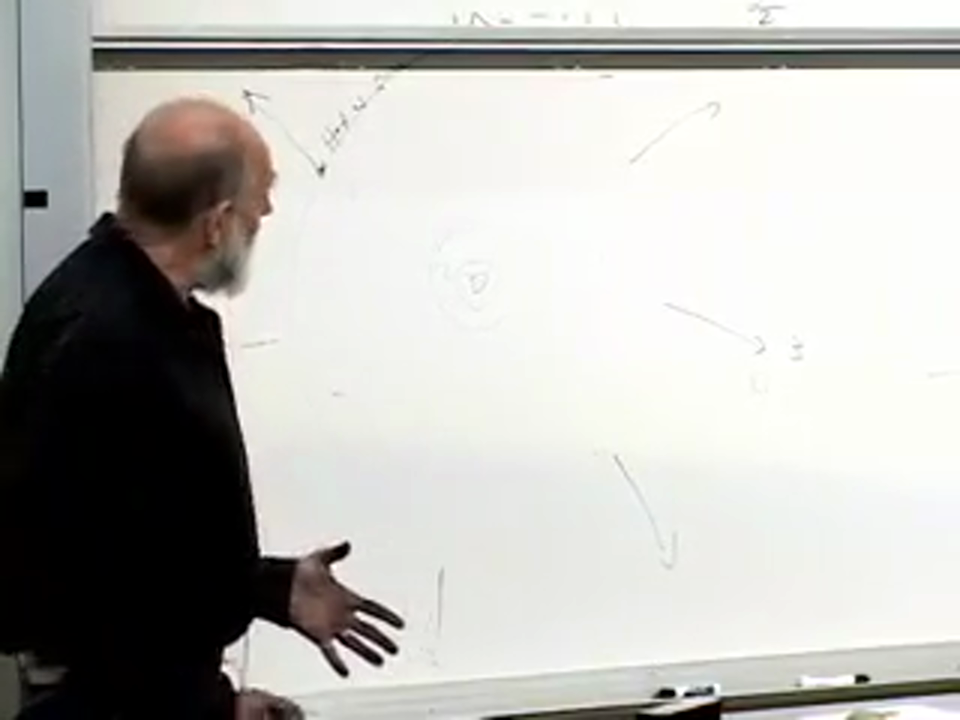
\includegraphics[width=0.72\textwidth]{lecture_09_figure_17.png}
  \caption{以观测者为中心的最后散射面及越来越远的壳层示意图。源帧位于01:42:05。}
  \label{fig:l09-last-scattering-board}
\end{figure}

\begin{figure}[H]
  \centering
  \begin{tikzpicture}[scale=0.9,>=Latex]
    \fill (0,0) circle (2pt) node[below] {observer};
    \draw[thick,orange!70!black] (0,0) circle (2.55);
    \node[orange!70!black,align=center] at (0,3.05)
      {surface of last scattering};
    \foreach \a in {25,75,145,210,285,335}{
      \draw[->,blue!60!black] ({2.55*cos(\a)},{2.55*sin(\a)}) --
        ({1.7*cos(\a)},{1.7*sin(\a)});
    }
    \draw[decorate,decoration={snake,amplitude=1.5pt,segment length=7pt},
      red!65!black,thick,->] (-2.5,0) -- (-0.15,0);
    \node[red!65!black,below] at (-1.35,-0.15)
      {redshifted photon};
  \end{tikzpicture}
  \caption{最后散射图像的清晰重建。}
  \label{fig:l09-last-scattering-clean}
\end{figure}

该辐射发射时具有热等离子体特征的光谱，到达我们时波长大约长了一千倍。用讲座中的多普勒语言来说，遥远的发射面迅速退行，其辐射被强烈红移。用几何语言来说，波在传播过程中被拉伸。两种图像编码了同一关系，
\begin{equation}
  1+z=\frac{\lambda_0}{\lambda_{\mathrm{em}}}
      =\frac{a_0}{a_{\mathrm{em}}}.
  \label{eq:l09-cosmological-redshift}
\end{equation}
\editorialnote{方程\eqref{eq:l09-cosmological-redshift}是讲座中拉伸描述和多普勒描述的标准定量形式。}

在更早的观测时代，最后散射球在相应的图像中会更近，而观测到的背景光子红移会更小，因此能量更高。随着宇宙时间推进，从那个早期等离子体到达共动观测者的光子波长越来越长。

\section{红移光子的能量去了哪里？}

\begin{classroomqa}
\audiencequestion{一个光子以能量\(h\nu_{\mathrm{em}}\)发射，到达时红移，能量更少。那部分差值发生了什么？}
\lecturerresponse{牛顿推导最初是一个能量方程。其宇宙学形式将膨胀率与物质能量密度联系起来，因此物质能量和膨胀不能作为分别守恒的账目来处理。讲座将丢失的光子能量描述为进入膨胀的动能记账。一个充满辐射的活塞使这个类比变得具体：辐射压将活塞向外推，光子波长增加，它们丢失的能量变成机械功和活塞的动能。}
\end{classroomqa}

\begin{figure}[H]
  \centering
  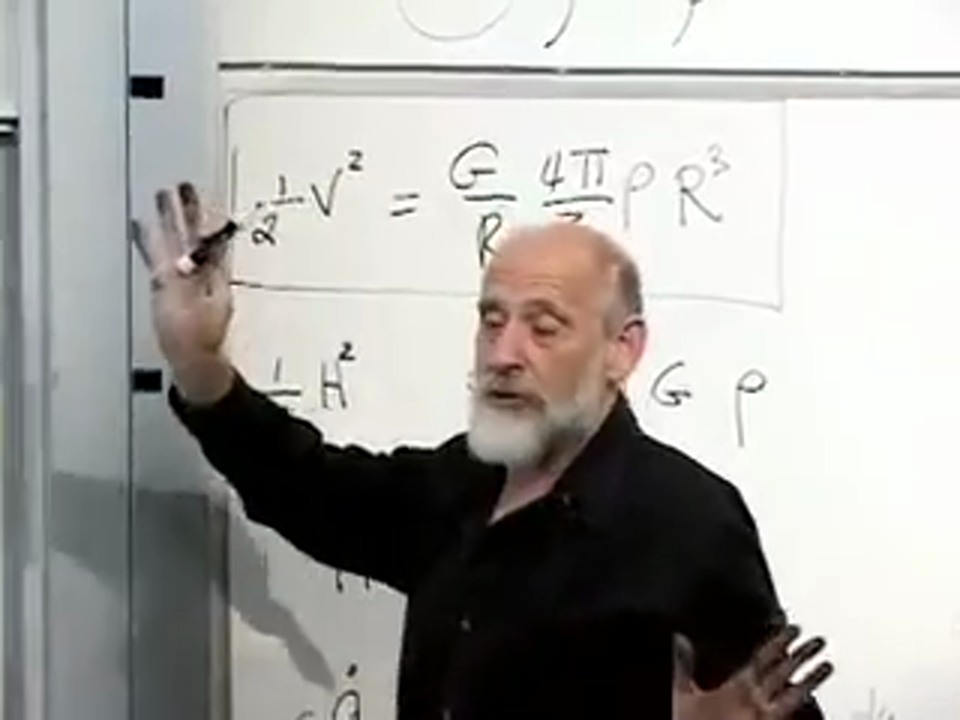
\includegraphics[width=0.72\textwidth]{lecture_09_figure_18.png}
  \caption{黑板上将方框中的牛顿能量方程置于相应的弗里德曼方程上方。源帧位于01:44:42。}
  \label{fig:l09-energy-bookkeeping-board}
\end{figure}

\begin{classroomqa}
\audiencequestion{是什么将辐射能量与膨胀耦合起来？}
\lecturerresponse{压强。在带有可移动活塞的圆柱体中，光子将动量传递给壁。当活塞移动时，辐射做功；其波长增大，能量下降。均匀膨胀的宇宙没有字面意义上的外部活塞，但\(p\,dV\)类比解释了为什么辐射的能量密度下降得比仅由数目稀释所导致的更快。}
\end{classroomqa}

\begin{figure}[H]
  \centering
  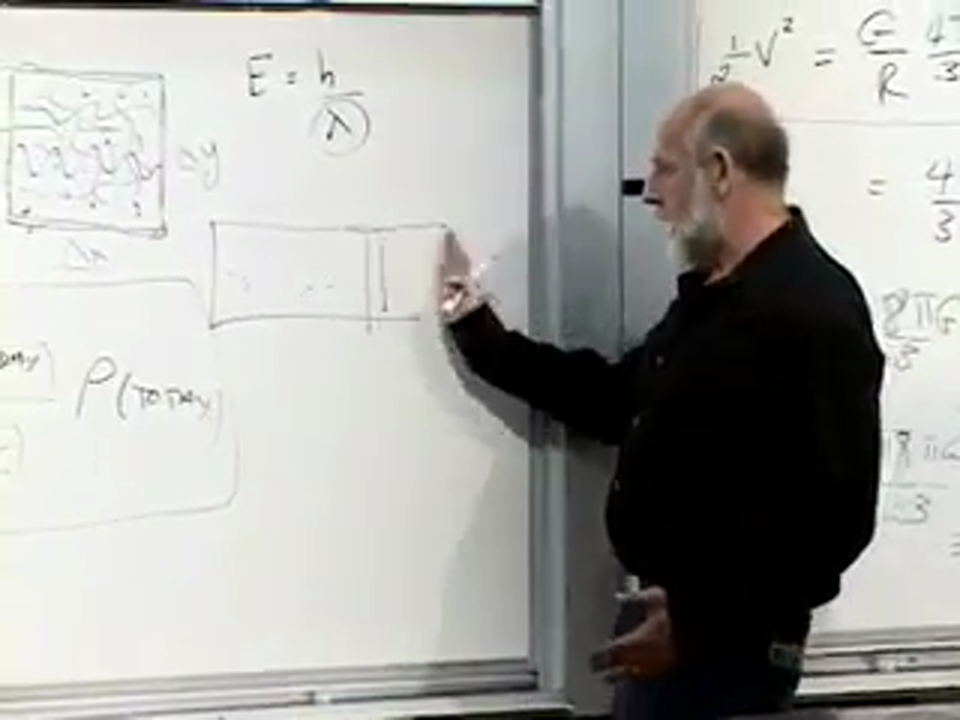
\includegraphics[width=0.72\textwidth]{lecture_09_figure_19.png}
  \caption{用于可视化压强做功的可移动充有光子的活塞。源帧位于01:46:40。}
  \label{fig:l09-piston-board}
\end{figure}

\begin{figure}[H]
  \centering
  \begin{tikzpicture}[scale=0.92,>=Latex]
    \draw[thick] (0,0) rectangle (5.3,2.6);
    \draw[very thick] (4.25,0) -- (4.25,2.6);
    \draw[very thick] (4.25,1.3) -- (5.25,1.3);
    \draw[->,thick,red!65!black] (5.25,1.3) -- (6.2,1.3)
      node[right] {moving piston};
    \foreach \y in {0.55,1.3,2.05}{
      \draw[decorate,decoration={snake,amplitude=1.4pt,segment length=6pt},
        blue!65!black,->] (0.35,\y) -- (3.9,\y);
    }
    \node at (2.15,-0.45) {radiation does \(p\,dV\) work};
  \end{tikzpicture}
  \caption{辐射-活塞类比的清晰重构。}
  \label{fig:l09-piston-clean}
\end{figure}

广义相对论中的能量需要谨慎处理。在一般的膨胀时空中，未必存在一个唯一的守恒全局能量，类似于孤立牛顿系统的能量。局域应力-能量守恒仍然成立，而对于均匀流体，它给出连续性方程
\begin{equation}
  \dot\rho+3H(\rho+p)=0,
  \label{eq:l09-continuity}
\end{equation}
其中包含压强做功项，正是物质与辐射标度律背后的原因。\editorialnote{方程 \eqref{eq:l09-continuity} 是讲座中刻意采用牛顿式能量记账类比所依据的精确局域广义相对论表述。}

真空能使得这一疑难尤为尖锐。由于其密度保持恒定而体积增大，共动区域内的总真空能增加。其负压强是引力源的一部分，并驱动加速膨胀。因此，不应要求朴素的“共动盒中的物质能量”单独守恒，而不把几何与压强做功包括在内。

\section{为什么标度因子可以从时间项中移除}

\begin{classroomqa}
\audiencequestion{为什么标度因子乘在度规的空间部分上，而不乘在时间部分上？}
\lecturerresponse{这是时间坐标的一种选择。假设从共形时间坐标 \(t\) 出发，有
\begin{equation}
  d\tau^2=A^2(t)\left(dt^2-dx^2\right).
\end{equation}
通过下式定义新的宇宙时间 \(T\)：
\begin{equation}
  dT=A(t)\,dt.
\end{equation}
于是
\begin{equation}
  d\tau^2=dT^2-A^2\bigl(t(T)\bigr)dx^2.
\end{equation}
时间微分前的公共因子已经消失，而物理标度因子仍留在空间项中。}
\end{classroomqa}

\begin{figure}[H]
  \centering
  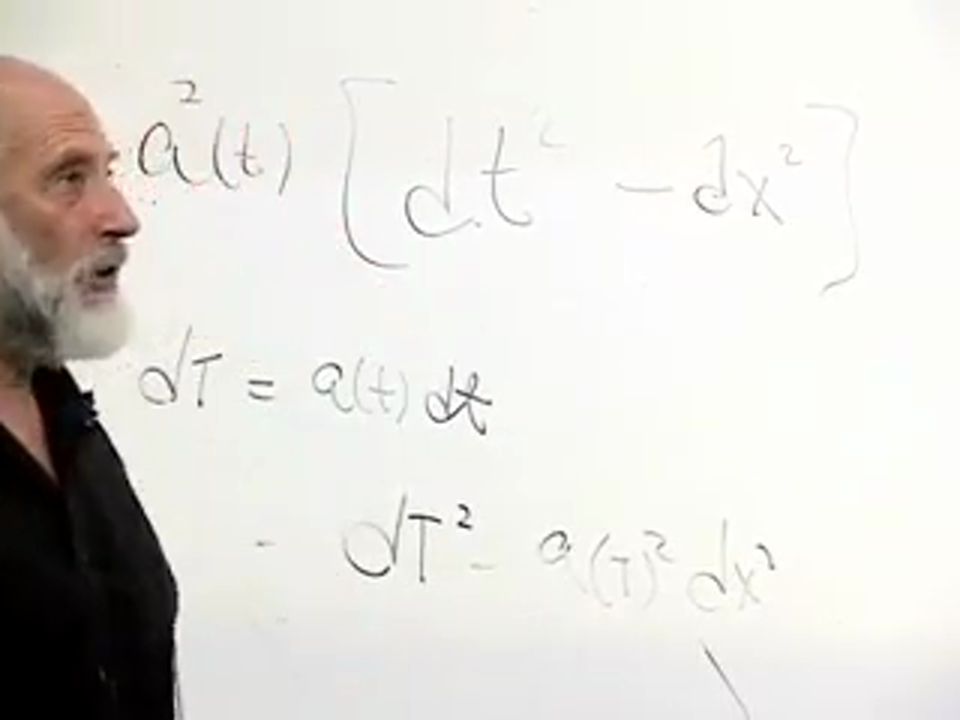
\includegraphics[width=0.72\textwidth]{lecture_09_figure_20.png}
  \caption{将共形时间转换为宇宙时间的时间重定义 \(dT=A(t)dt\)。源帧在 01：51：05。}
  \label{fig:l09-time-reparam-board}
\end{figure}

\section{曲率、真空能与宇宙命运}

\begin{classroomqa}
\audiencequestion{如果宇宙是正曲率的，我们是否应该已经看到星系朝我们运动而来？}
\lecturerresponse{未必。一个以低于逃逸速度发射的抛射体先向外运动，到达一个转折点，之后才落回。我们是在宇宙的膨胀阶段观测它。如果没有真空能，一个正曲率的物质宇宙最终会再坍缩。足够大的正真空能会阻止这一转折，而观测值似乎大到足以使长期膨胀呈指数式，无论空间曲率有多小。}
\end{classroomqa}

指数式的未来并非能量天堂。恒星最终会燃尽，物质与辐射密度呈指数式下降，遥远区域将超出因果接触。真空能仍然存在，而普通结构则变得越来越冷、越来越稀薄。

\begin{classroomqa}
\audiencequestion{向更遥远的过去看，光子是否比普通粒子更多？}
\lecturerresponse{光子与重子的数密度之比已经极其巨大，按讲座中的估计约为每个重子 \(10^{10}\) 个光子，而共动体积中的这两个数目都近似保持不变。向过去回溯时改变的主要是每个光子的能量。光子能量按 \(a^{-1}\) 上升，而非相对论性静止质量则不然。因此，尽管数目比本身未必改变，辐射在早期仍主导能量密度。}
\end{classroomqa}

核心教训是，仅凭几何并不能决定宇宙的历史。平坦的弗里德曼方程给出了膨胀与能量密度之间的关系，但物质内容提供了时间依赖关系。非相对论性物质给出 \(a\propto t^{2/3}\)，辐射给出 \(a\propto t^{1/2}\)，而恒定的真空能给出指数式膨胀。这三条定律组织了宇宙相继的各个时代，并解释了为什么同一个标度因子控制着距离、红移以及不断变化的哈勃参数。

\end{document}
